\subsection{Desenvolvimento}

\begin{frame}
	\frametitle{Simulação}
	\begin{block}{Simiam}
		\begin{itemize}
		  \item Simulador implementado no Matlab.
		  \item Implementado como sistema híbrido (Supervisor escalona controladores).
		\end{itemize}
	\end{block}
	\onslide<2>
	\begin{figure}[h]
\centering
\caption{Robôs Khepera 3 e QuickBot}
\label{fig:RobosK3QB}
	\begin{subfigure}[b]{0.49\textwidth}%
		\centering
		% fbox{}
		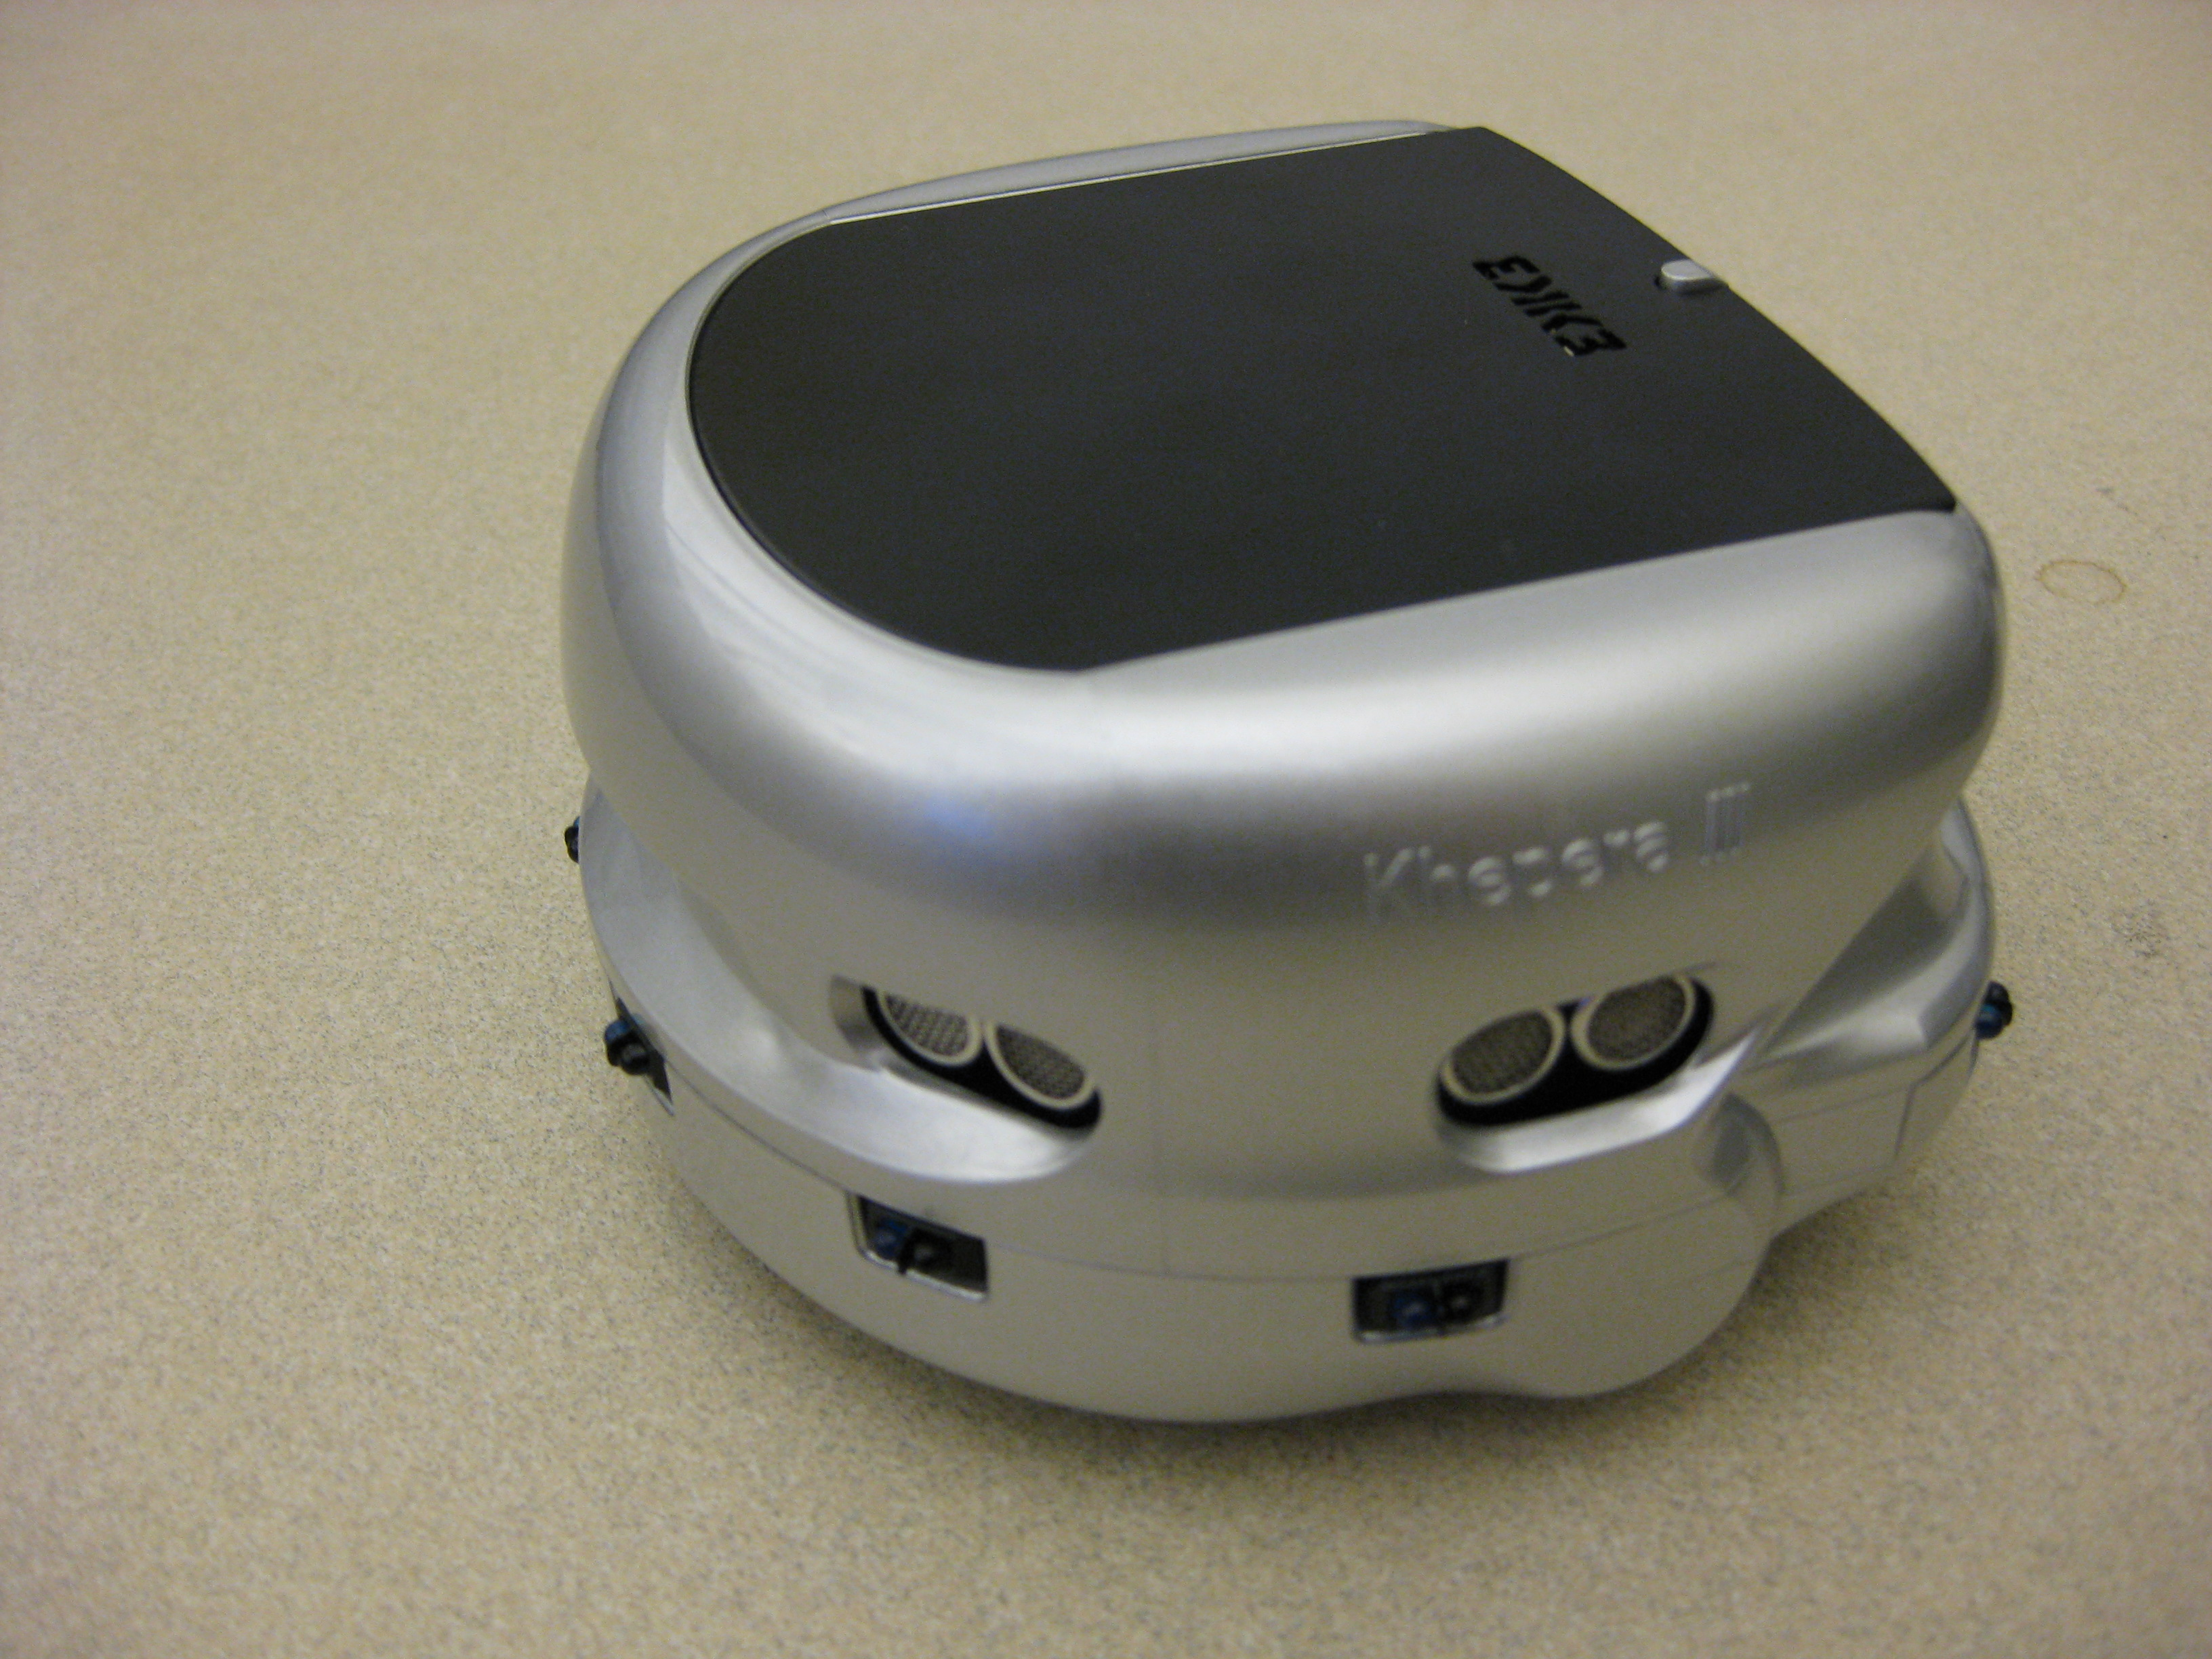
\includegraphics[trim= 8cm 0cm 0cm 0cm,clip,
scale=0.14]{Figuras/Khepera_III_robot}
		\subcaption{Robô Khepera 3}
	  	\label{fig:test1}
	\end{subfigure}
	~
	\begin{subfigure}[b]{0.49\textwidth}%
		\centering
		% fbox{}
		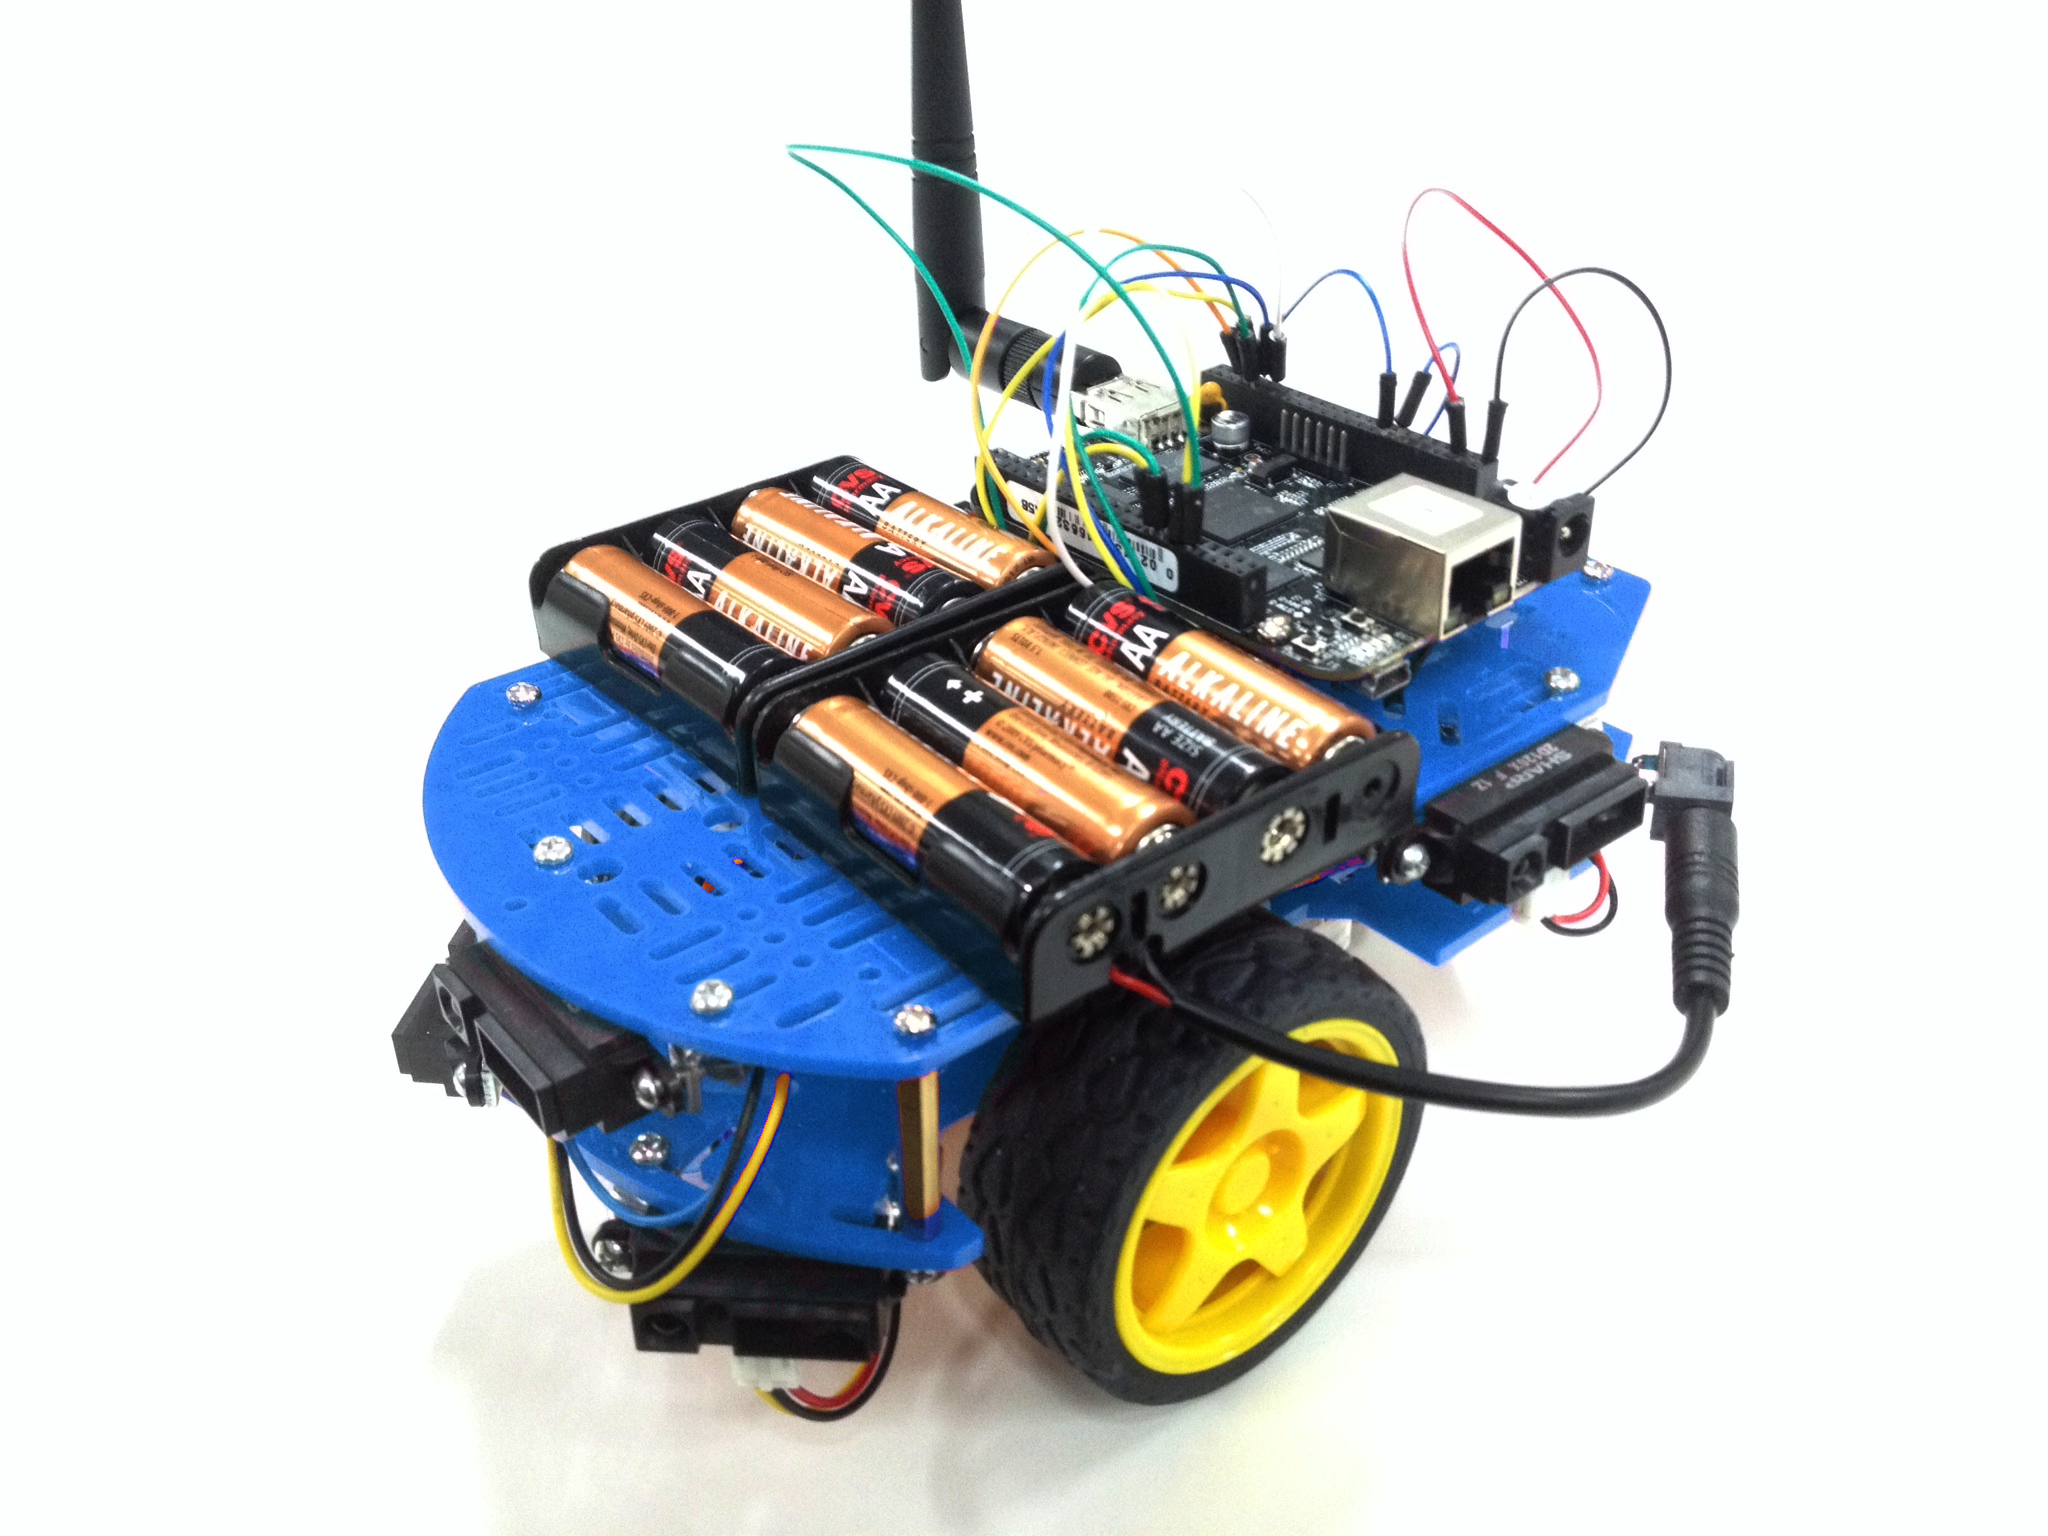
\includegraphics[trim={6cm 0cm 3cm 0cm},clip,
scale=0.09]{Figuras/quickbot-blue}
		\subcaption{Robô QuickBot}
	  	\label{fig:test2}
	\end{subfigure}
	
	\textbf{Fonte: \citeonline{im:Khepera}, \citeonline{im:QuickBot_Blue}}
\end{figure}


%		\begin{figure}[!htb]
%			\centering
%			\caption{Robôs Khepera e QuickBot fisicamente e em simulação}
%			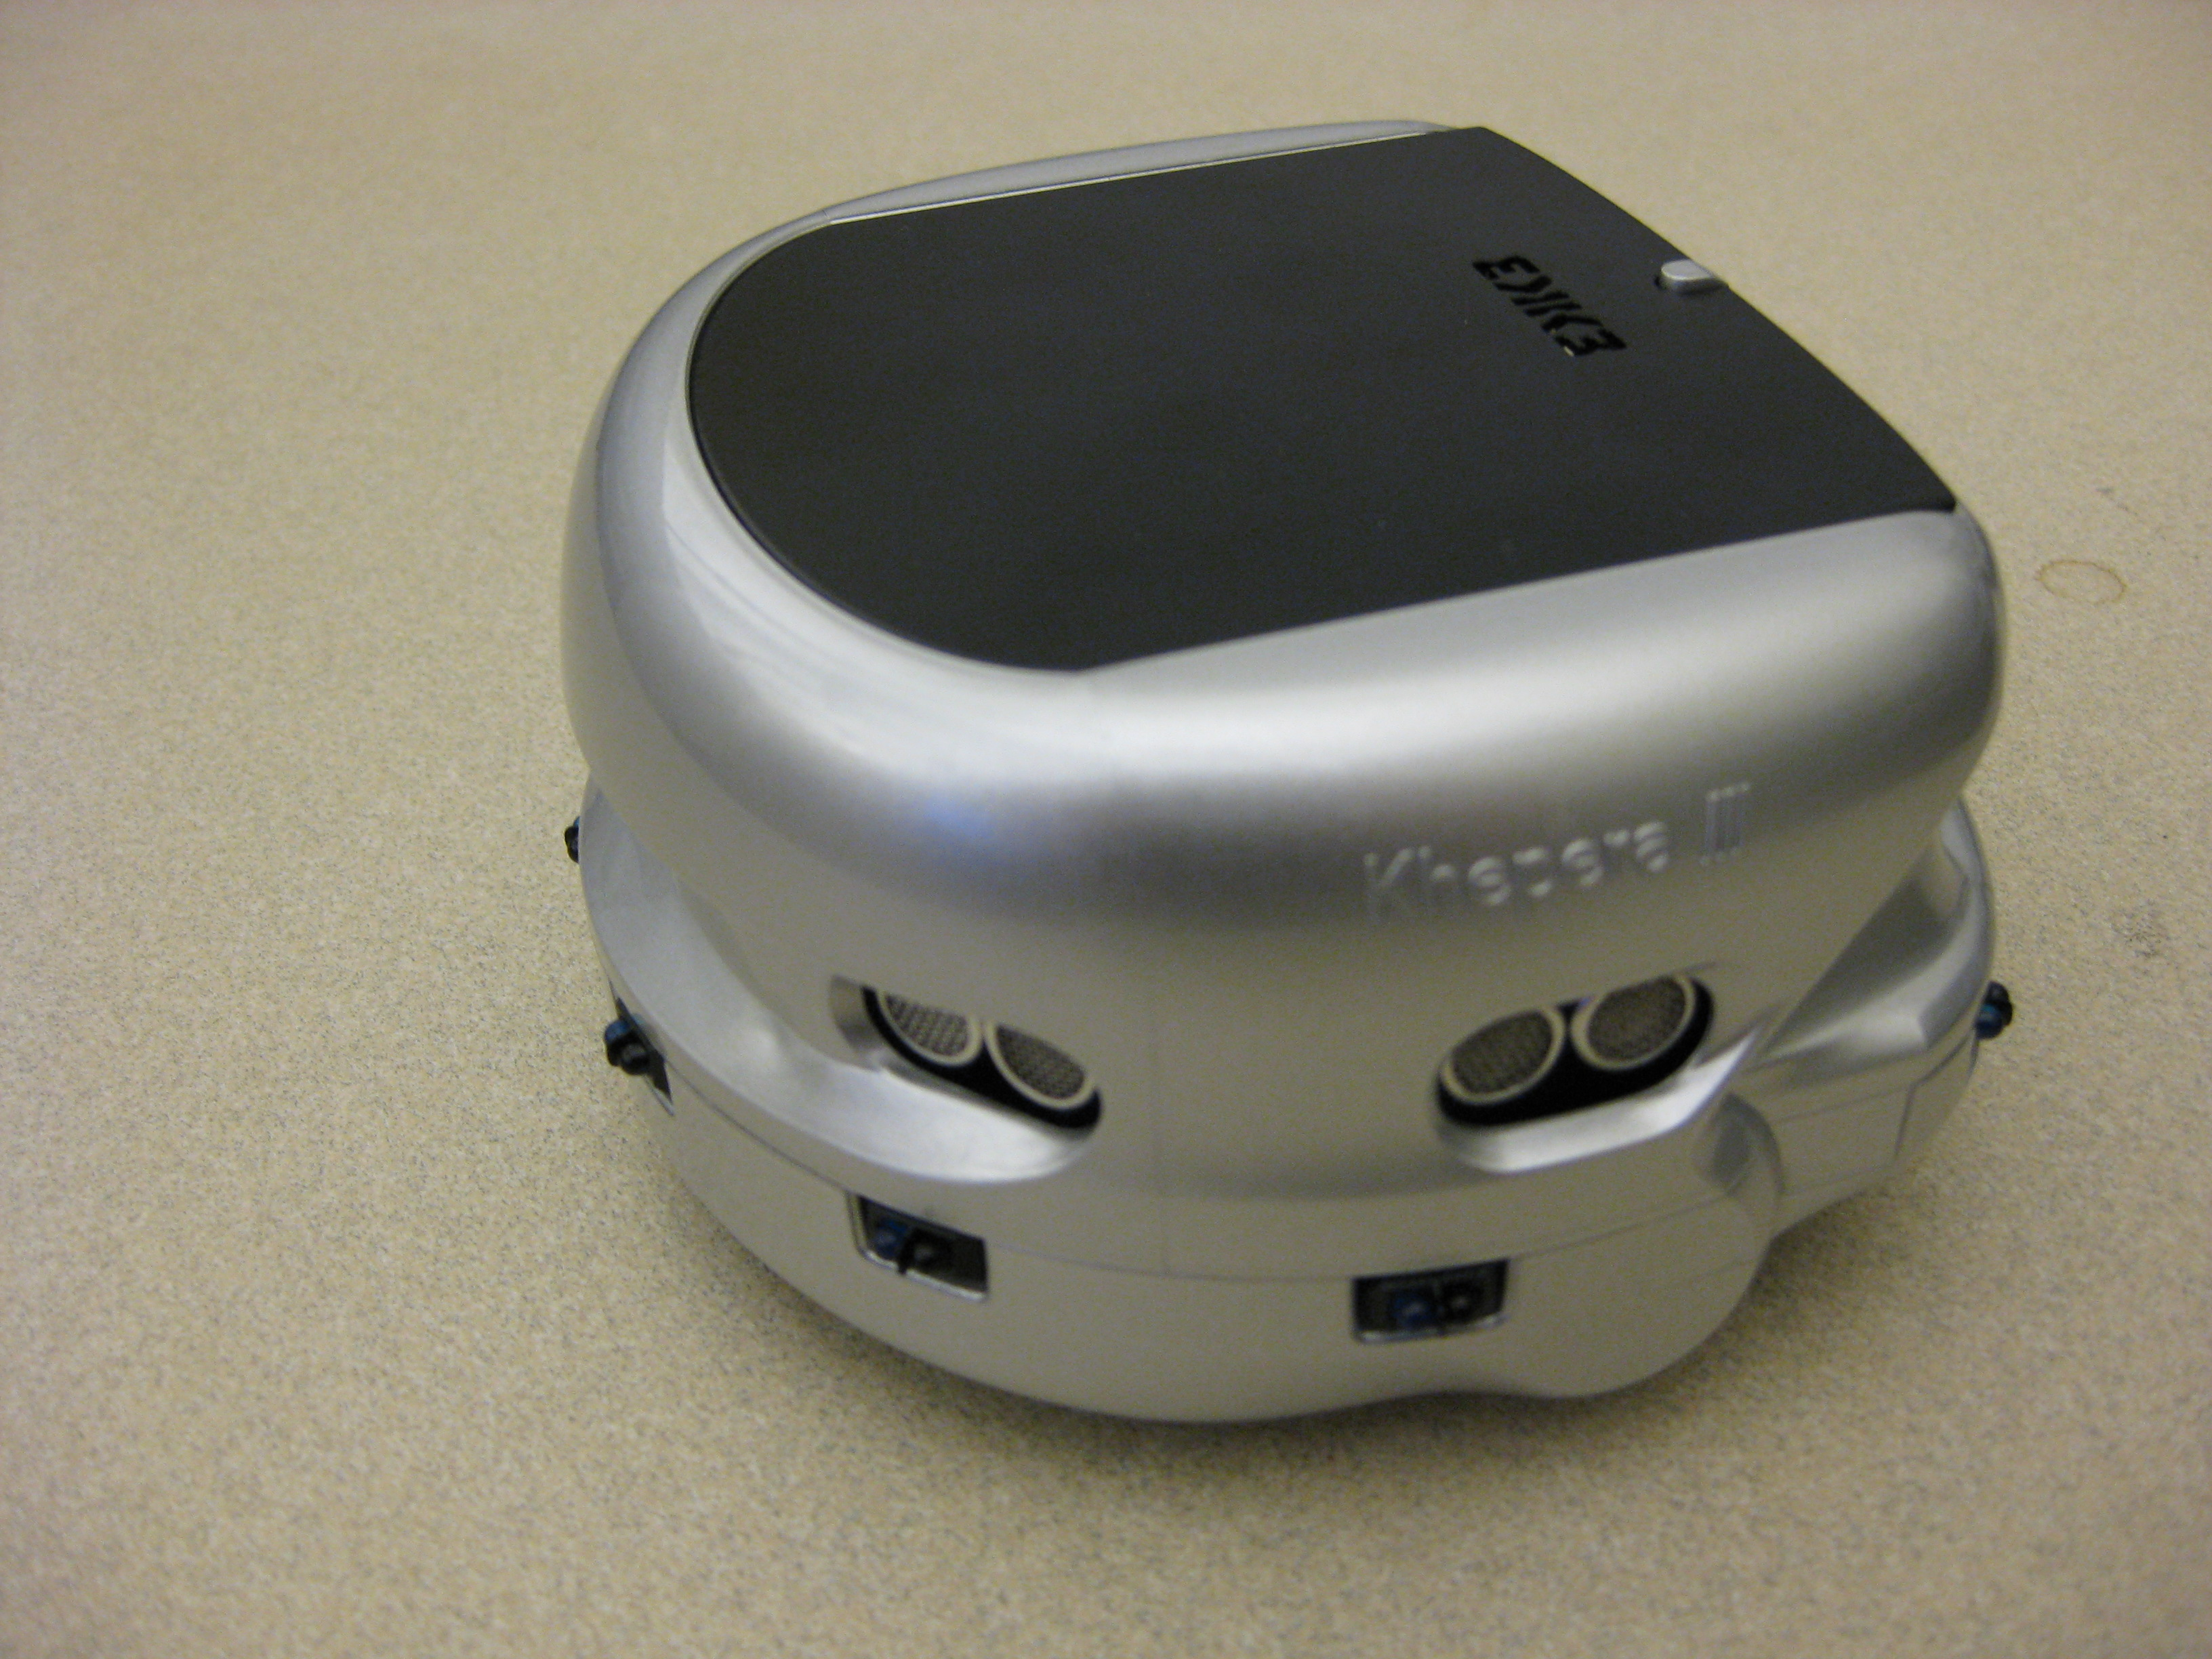
\includegraphics[trim={0cm 0cm 0cm 0cm},clip,
%scale=0.35]{Figuras/Khepera_III_robot}
%			%\vspace{-0.4cm}
%			\label{fig:RobosESim}
%		\end{figure}

%		\begin{figure}[!htb]
%			\centering			
%			\caption{Robôs Khepera e QuickBot fisicamente e em simulação}
%			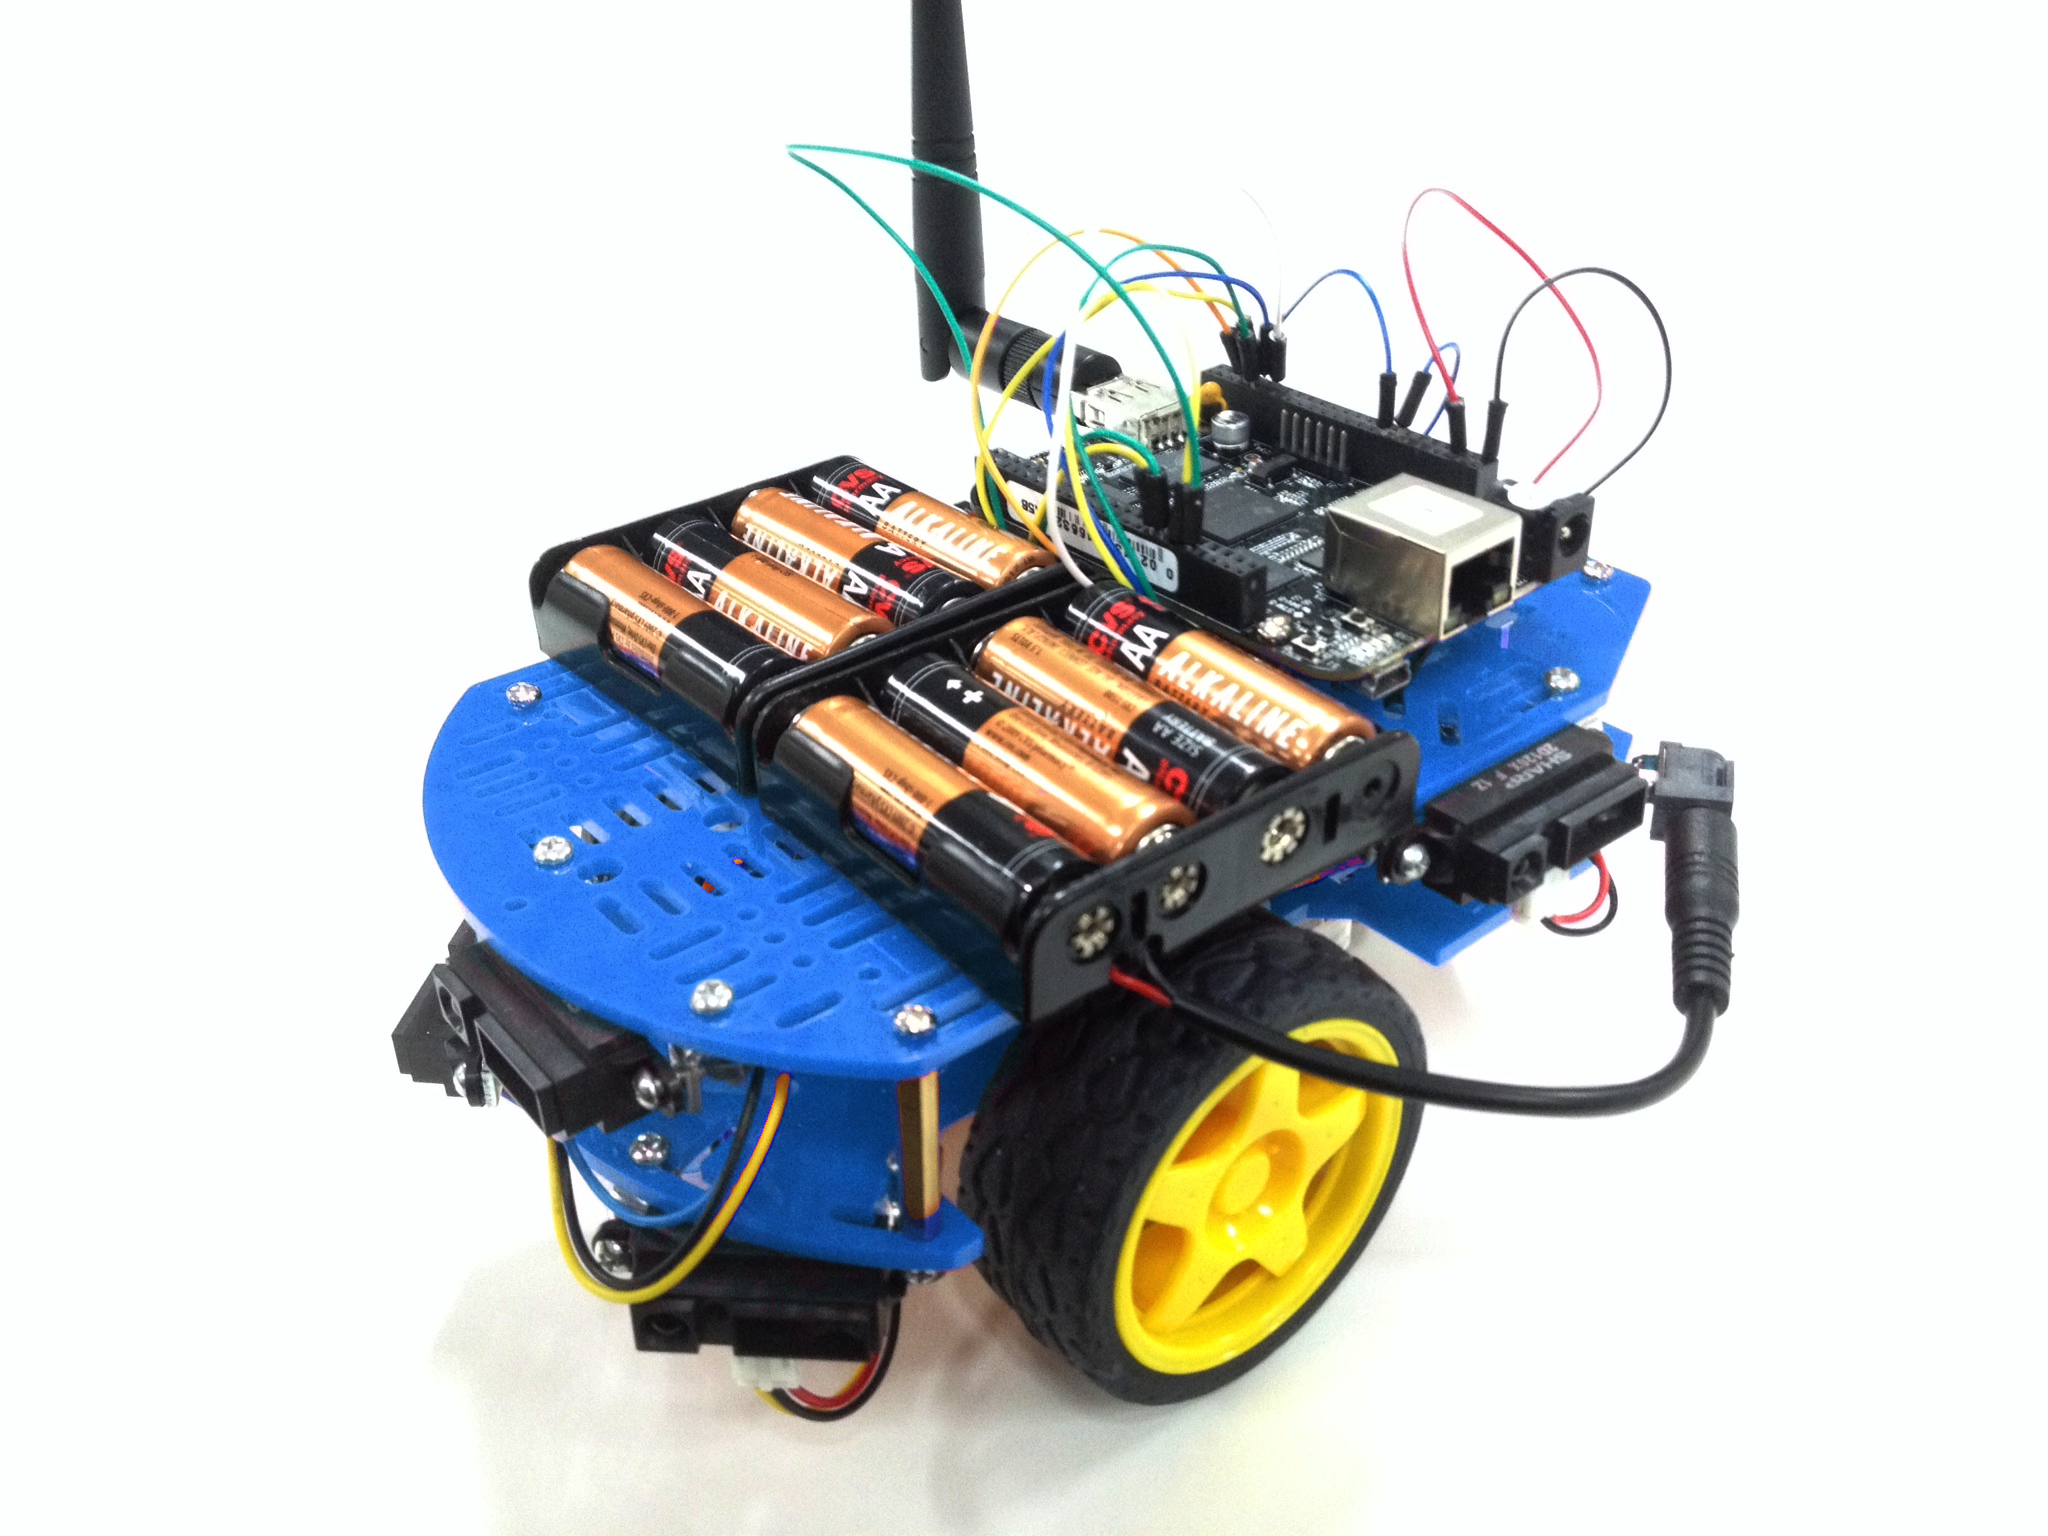
\includegraphics[trim={0cm 0cm 0cm 0cm},clip,
%scale=0.25]{Figuras/quickbot-blue}
%			%\vspace{-0.4cm}
%			\label{fig:RobosESim}
%		\end{figure}

%		\begin{figure}[!htb]
%			\centering
%			\caption{Robôs Khepera e QuickBot fisicamente e em simulação}
%			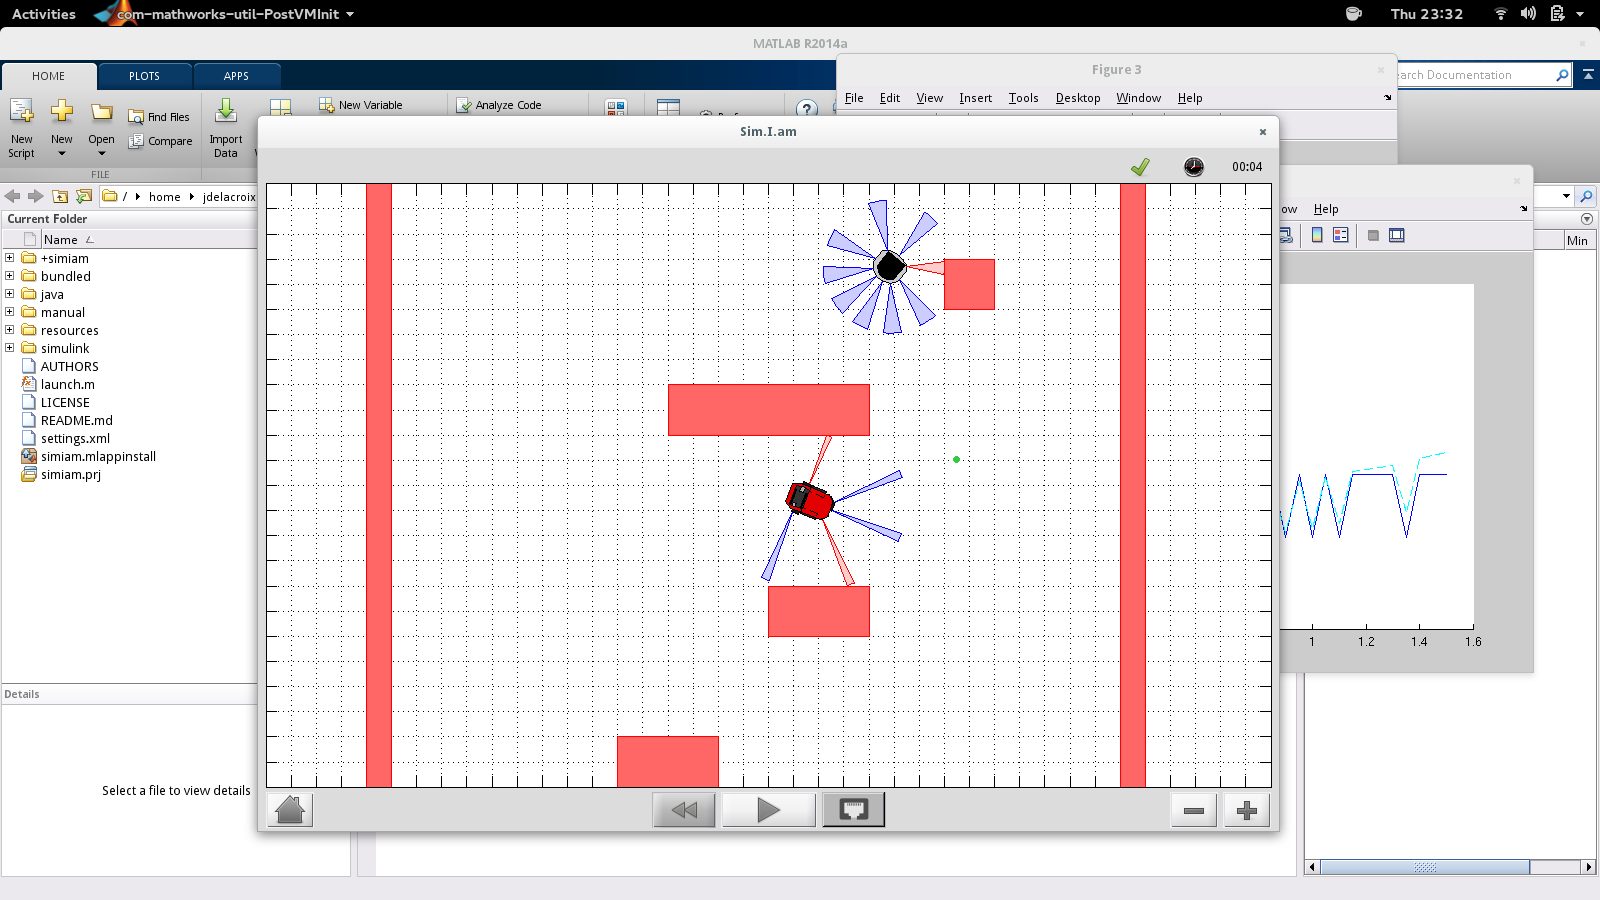
\includegraphics[trim={0cm 0cm 0cm 0cm},clip,
%scale=0.25]{Figuras/simiam-screenshot}
%			%\vspace{-0.4cm}
%			\label{fig:RobosESim}
%		\end{figure}


%\begin{figure}
%\begin{minipage}[c][11cm][t]{.5\textwidth}
%  \vspace*{\fill}
%  \centering
%  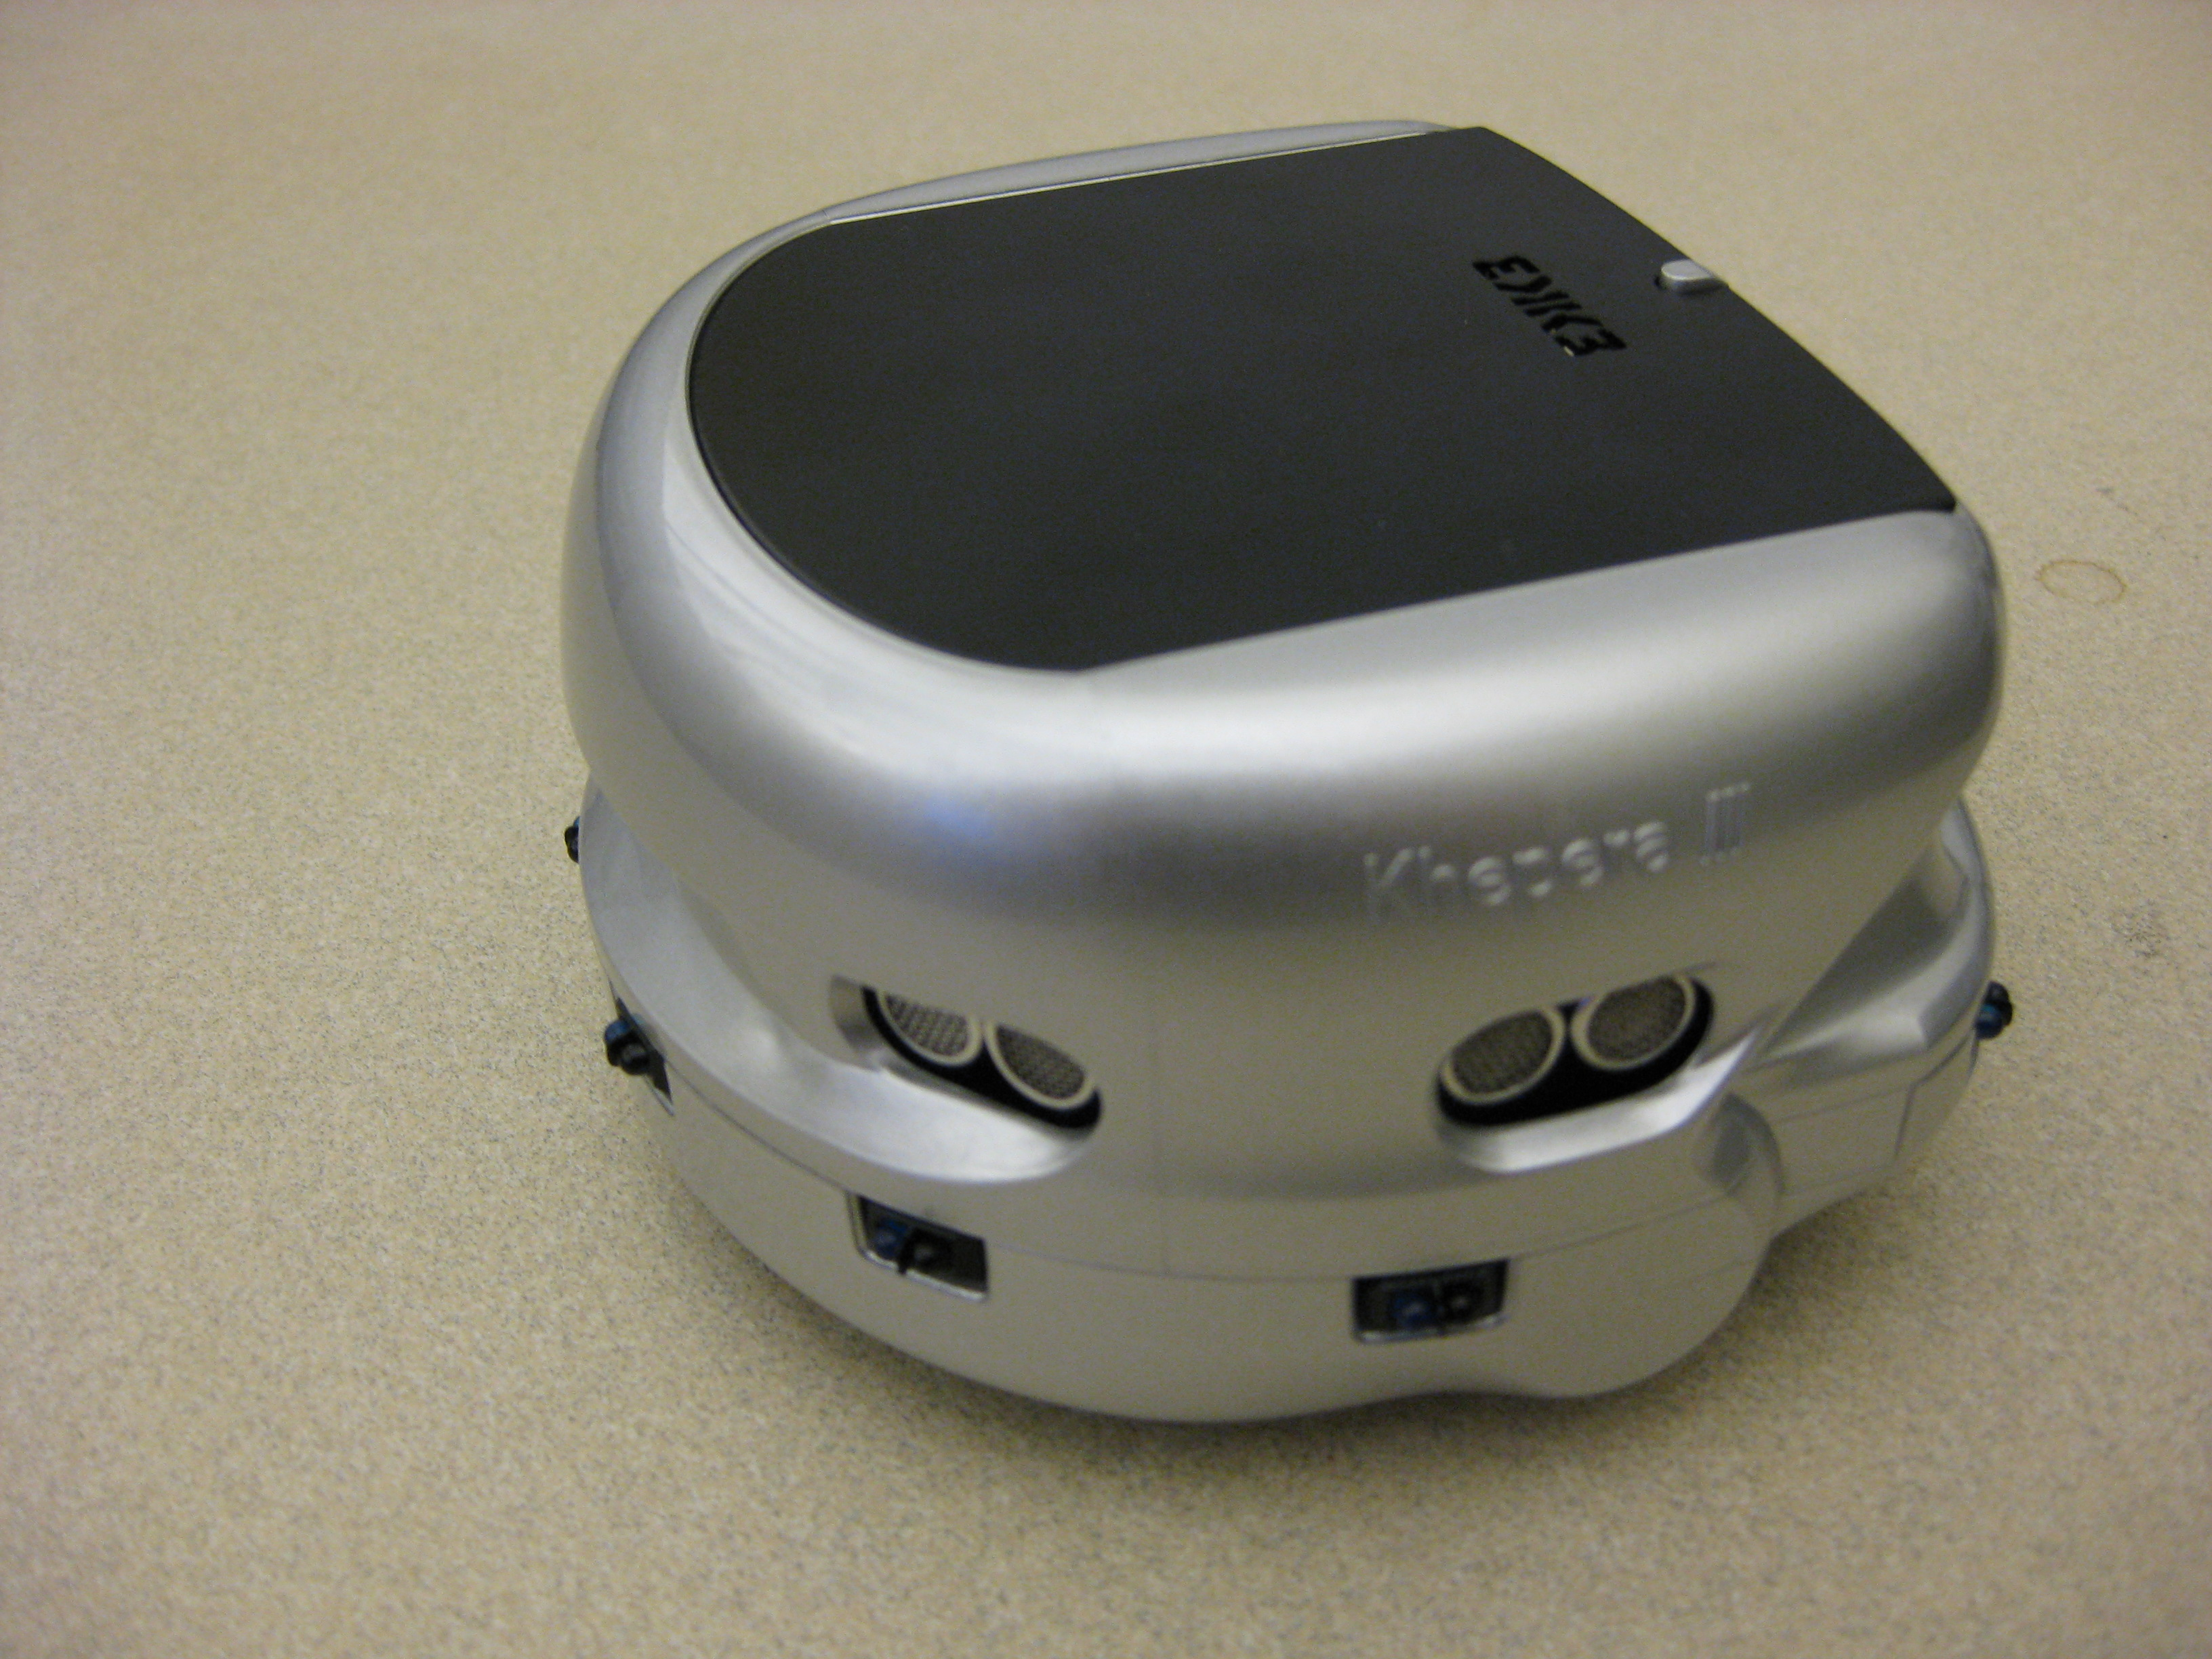
\includegraphics[width=5cm,height=4.5cm]{Figuras/Khepera_III_robot}
%  \subcaption{Robô Khepera}
%  \label{fig:test2}\par\vfill
%  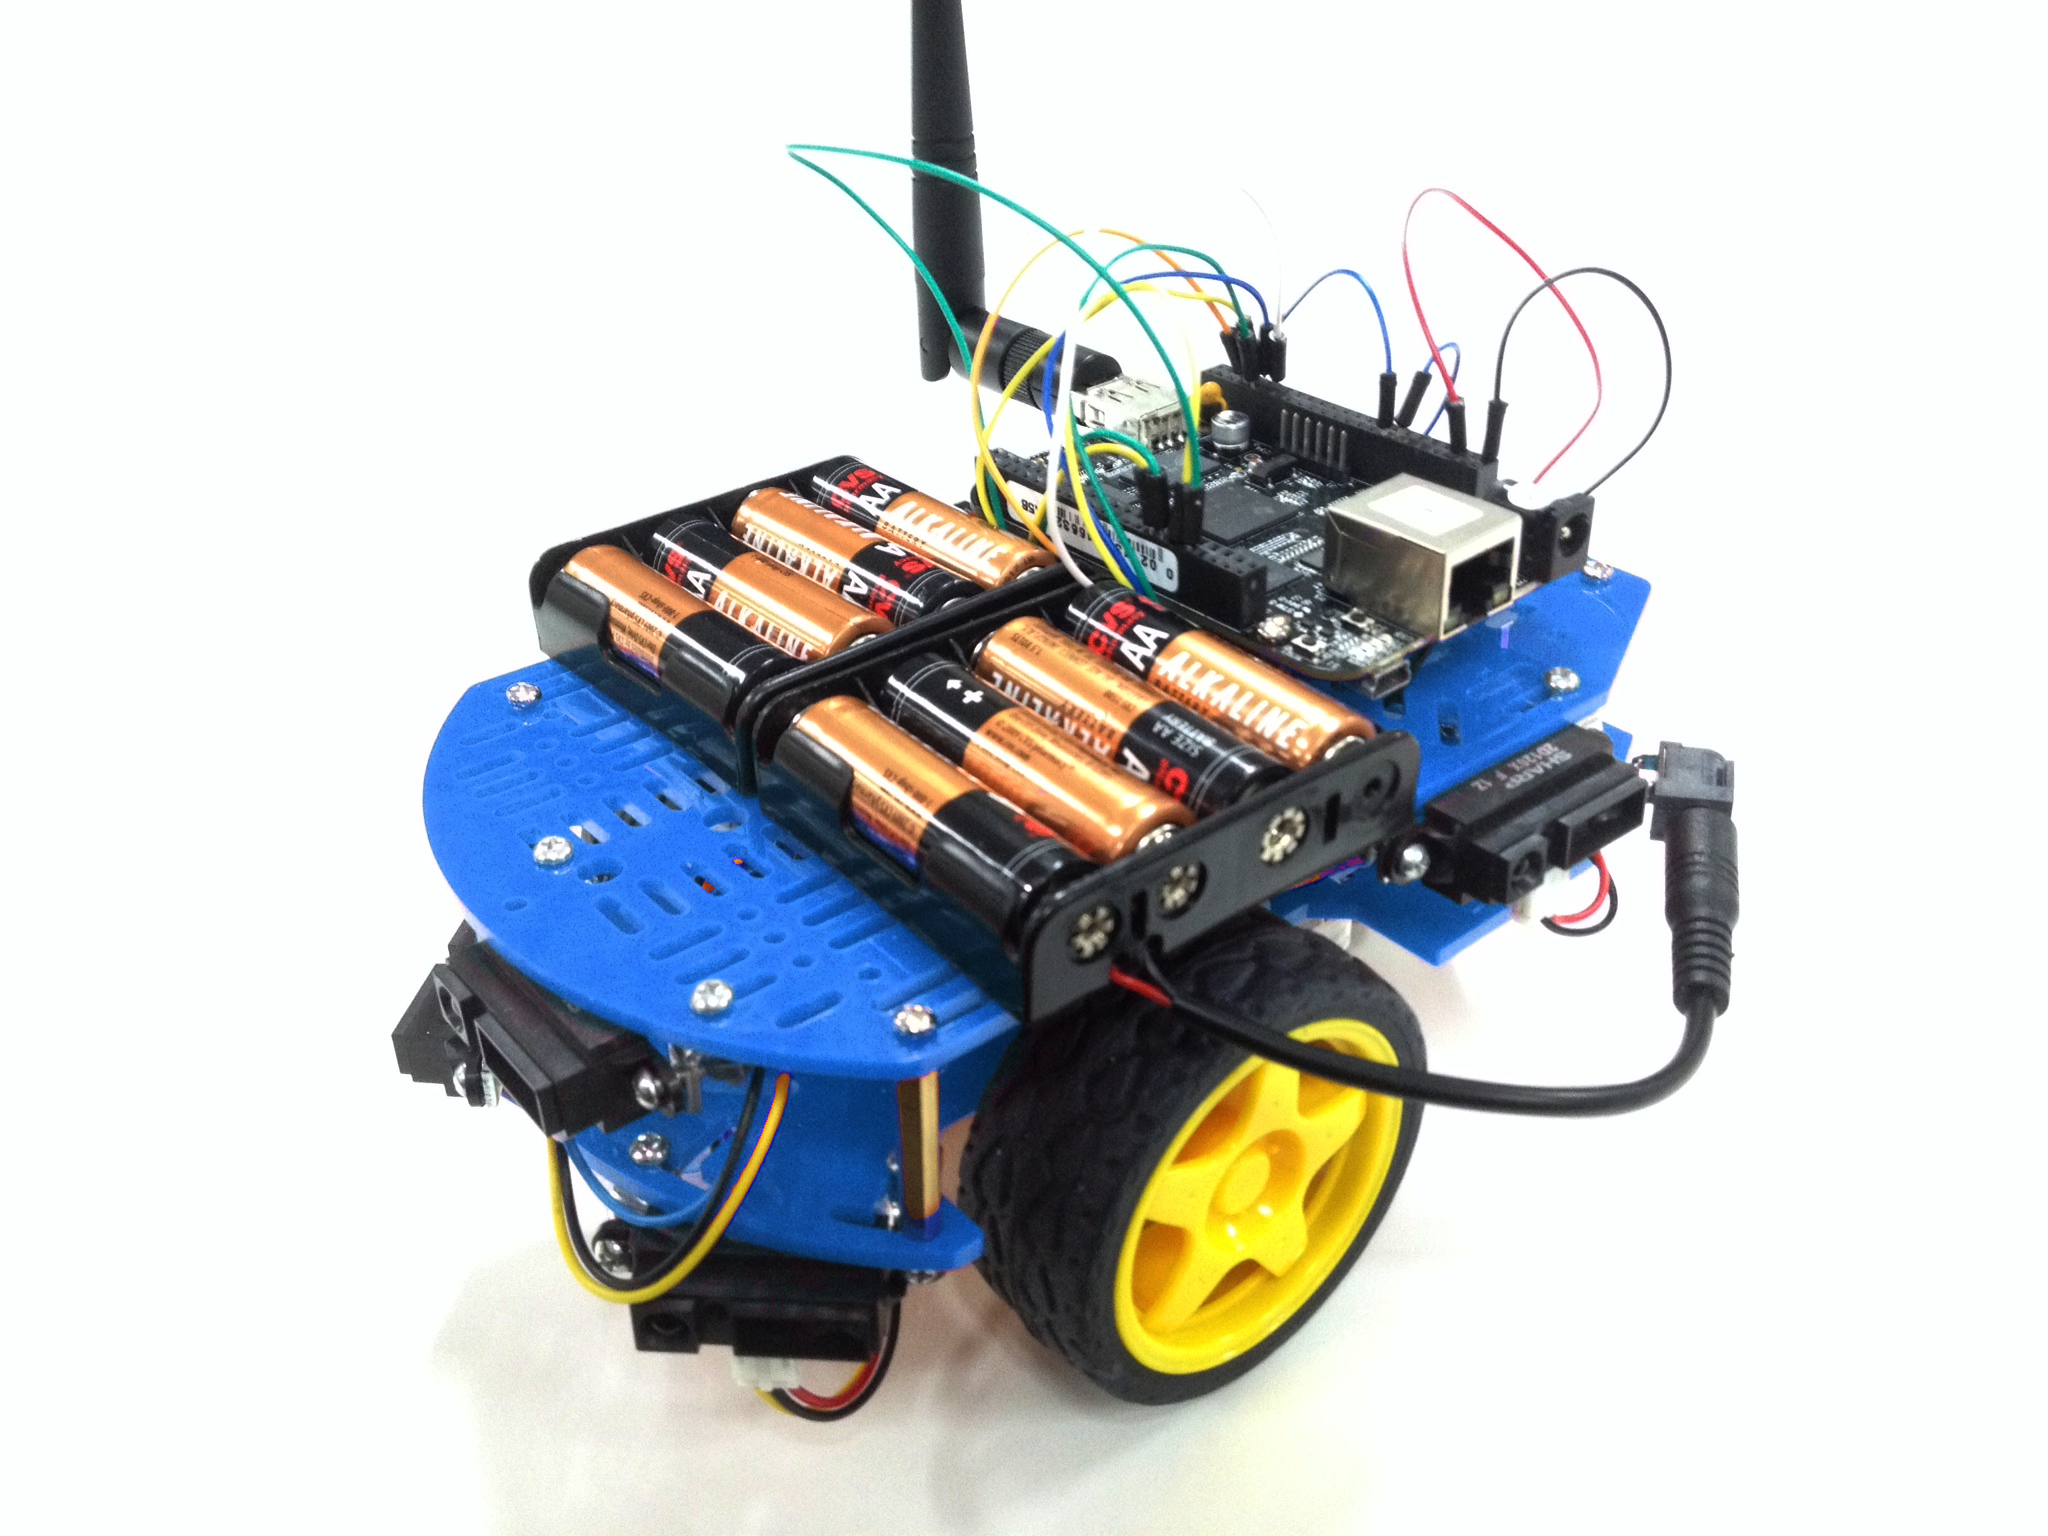
\includegraphics[width=5cm,height=4.5cm]{Figuras/quickbot-blue}
%  \subcaption{Robô QuickBot}
%  \label{fig:test3}
%\end{minipage}
%\begin{minipage}[c][11cm][t]{.5\textwidth}
%  \vspace*{\fill}
%  \centering
%  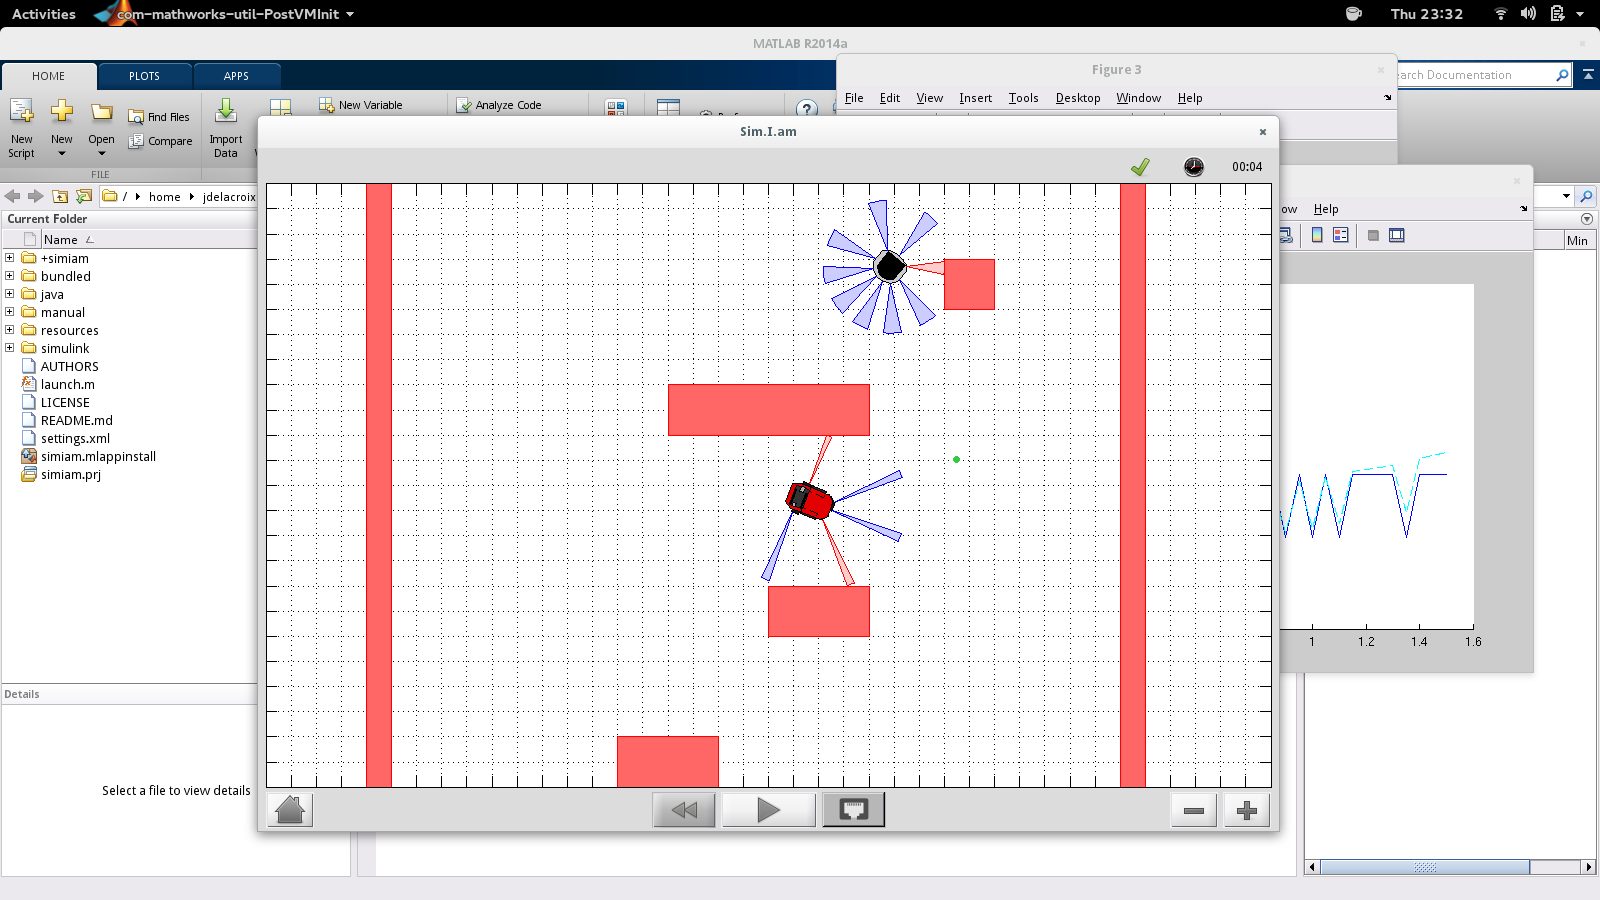
\includegraphics[width=5cm,height=10cm]{Figuras/simiam-screenshot}
%  \subcaption{Simulador Simiam}
%  \label{fig:test1}
%\end{minipage}%
%\end{figure}
	\onslide<3>
	\vspace{-3.5cm}
	\begin{figure}[h]
\centering
%\caption{Robôs Khepera 3 e QuickBot em simulação}
\label{fig:RobosEmSimulador}
		\centering
		% fbox{}
		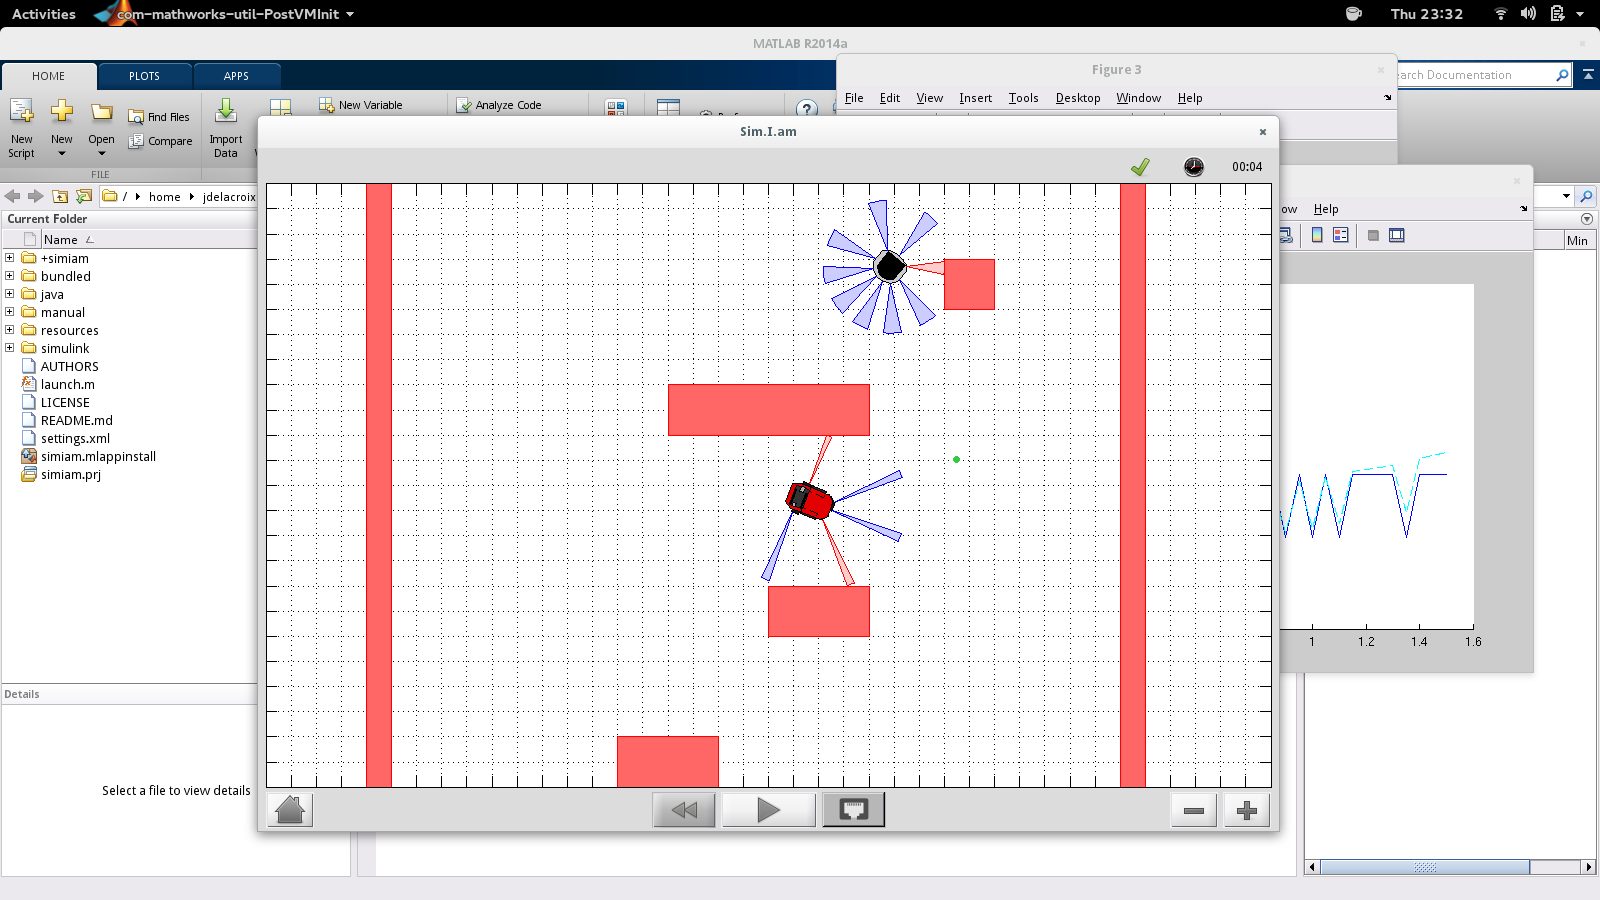
\includegraphics[trim={0cm 0cm 0cm 0cm},clip,
scale=0.16]{Figuras/simiam-screenshot}
	
	%\textbf{Fonte: \citeonline{im:Simiam}}
\end{figure}
\end{frame}
	
\begin{frame}
	\begin{exampleblock}{Alterações mais importantes}
		\begin{itemize}
		  \item Incluir uma classe para implementar aspectos físicos do robô deste
		  trabalho.
		  \item Incluir suporte para controladores \textit{fuzzy}.
		\end{itemize}
	\end{exampleblock}
\end{frame}

\begin{frame}
	\frametitle{Especificações}
	\begin{figure}[h]
	\centering
	\caption{Resposta do sensor infravermelho}
	\label{fig:SensorIR}
	
	%\fbox{}
	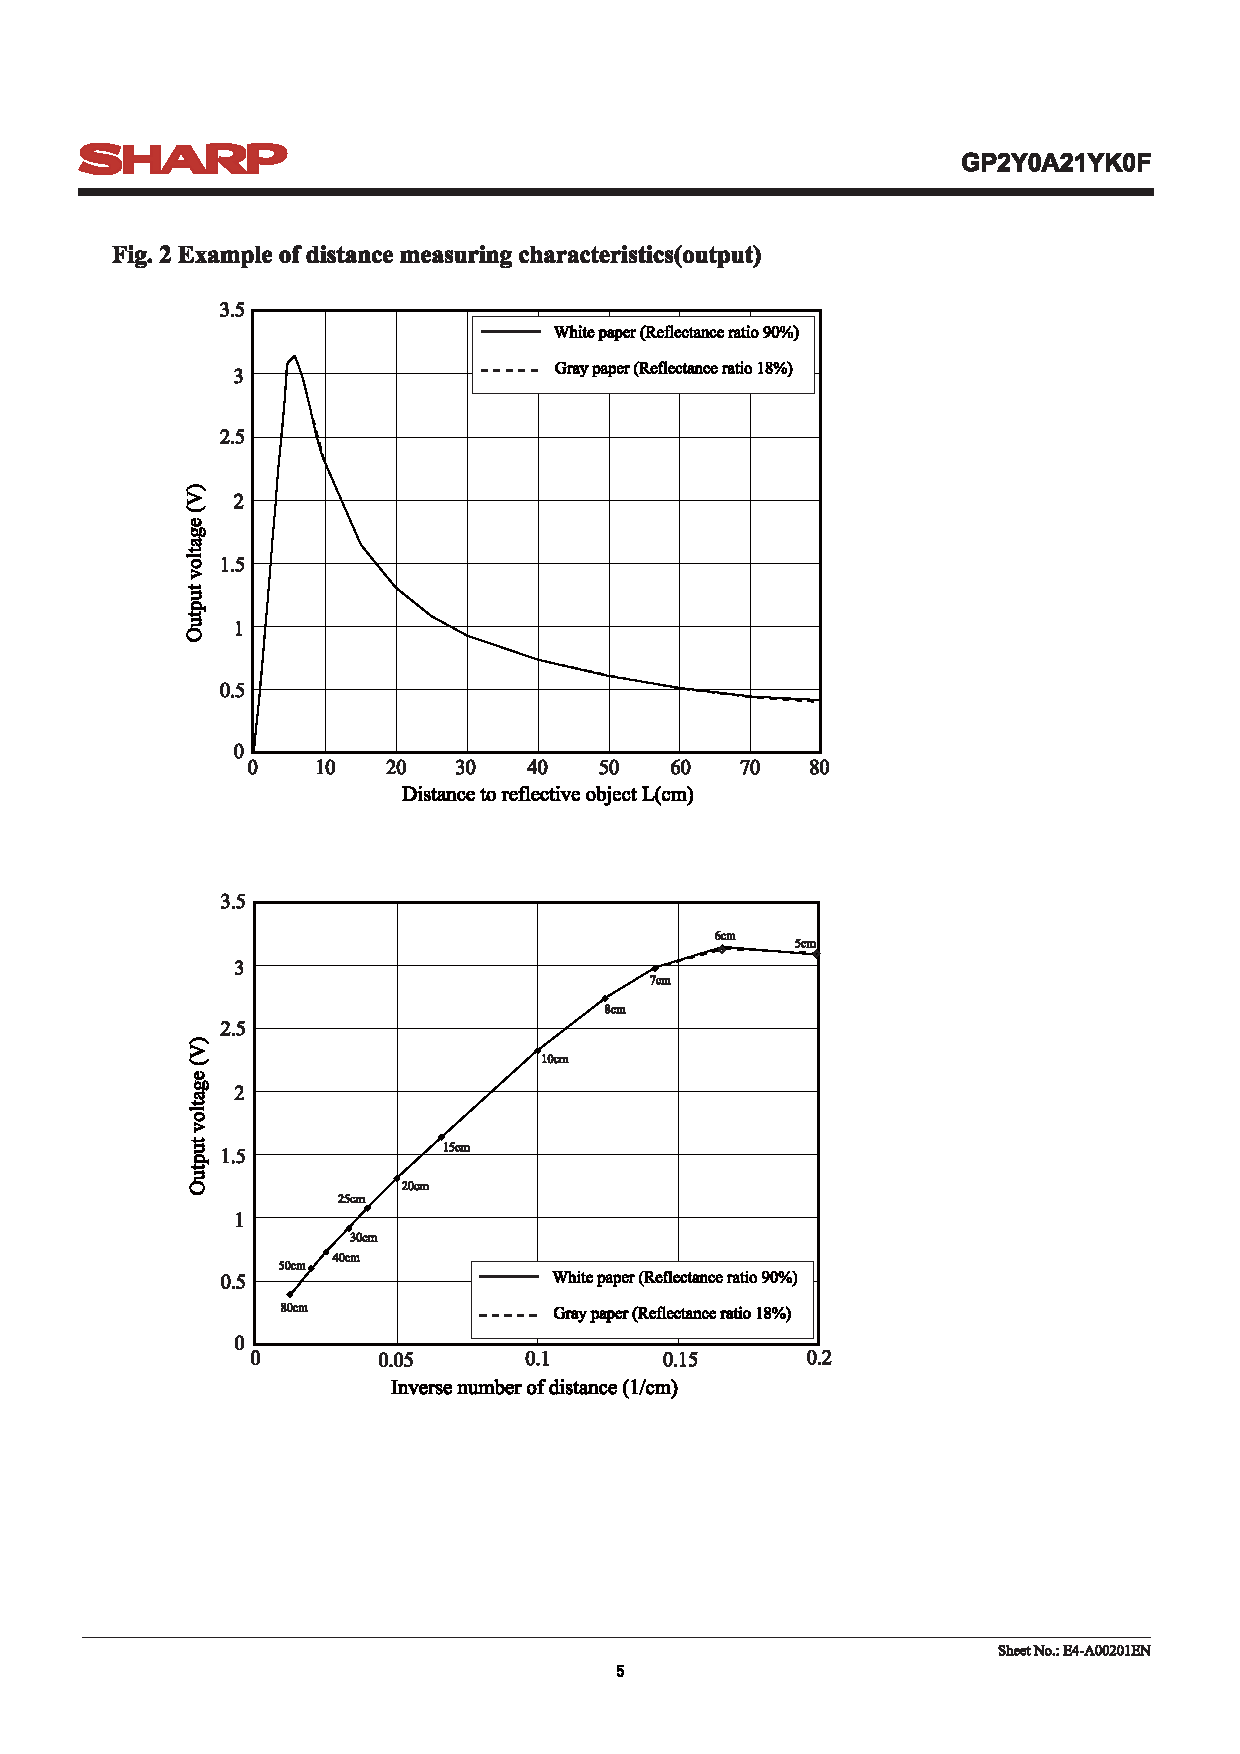
\includegraphics[trim= 3cm 15.8cm 6.5cm 4.8cm,clip,
scale=1]{Figuras/IR_Datasheet_Figure}

	%\begin{tikzpicture}[auto, node distance=2cm, on grid,
%>=latex']%
	
	%\node[anchor=south west,inner sep=0] (image) at (0,0) {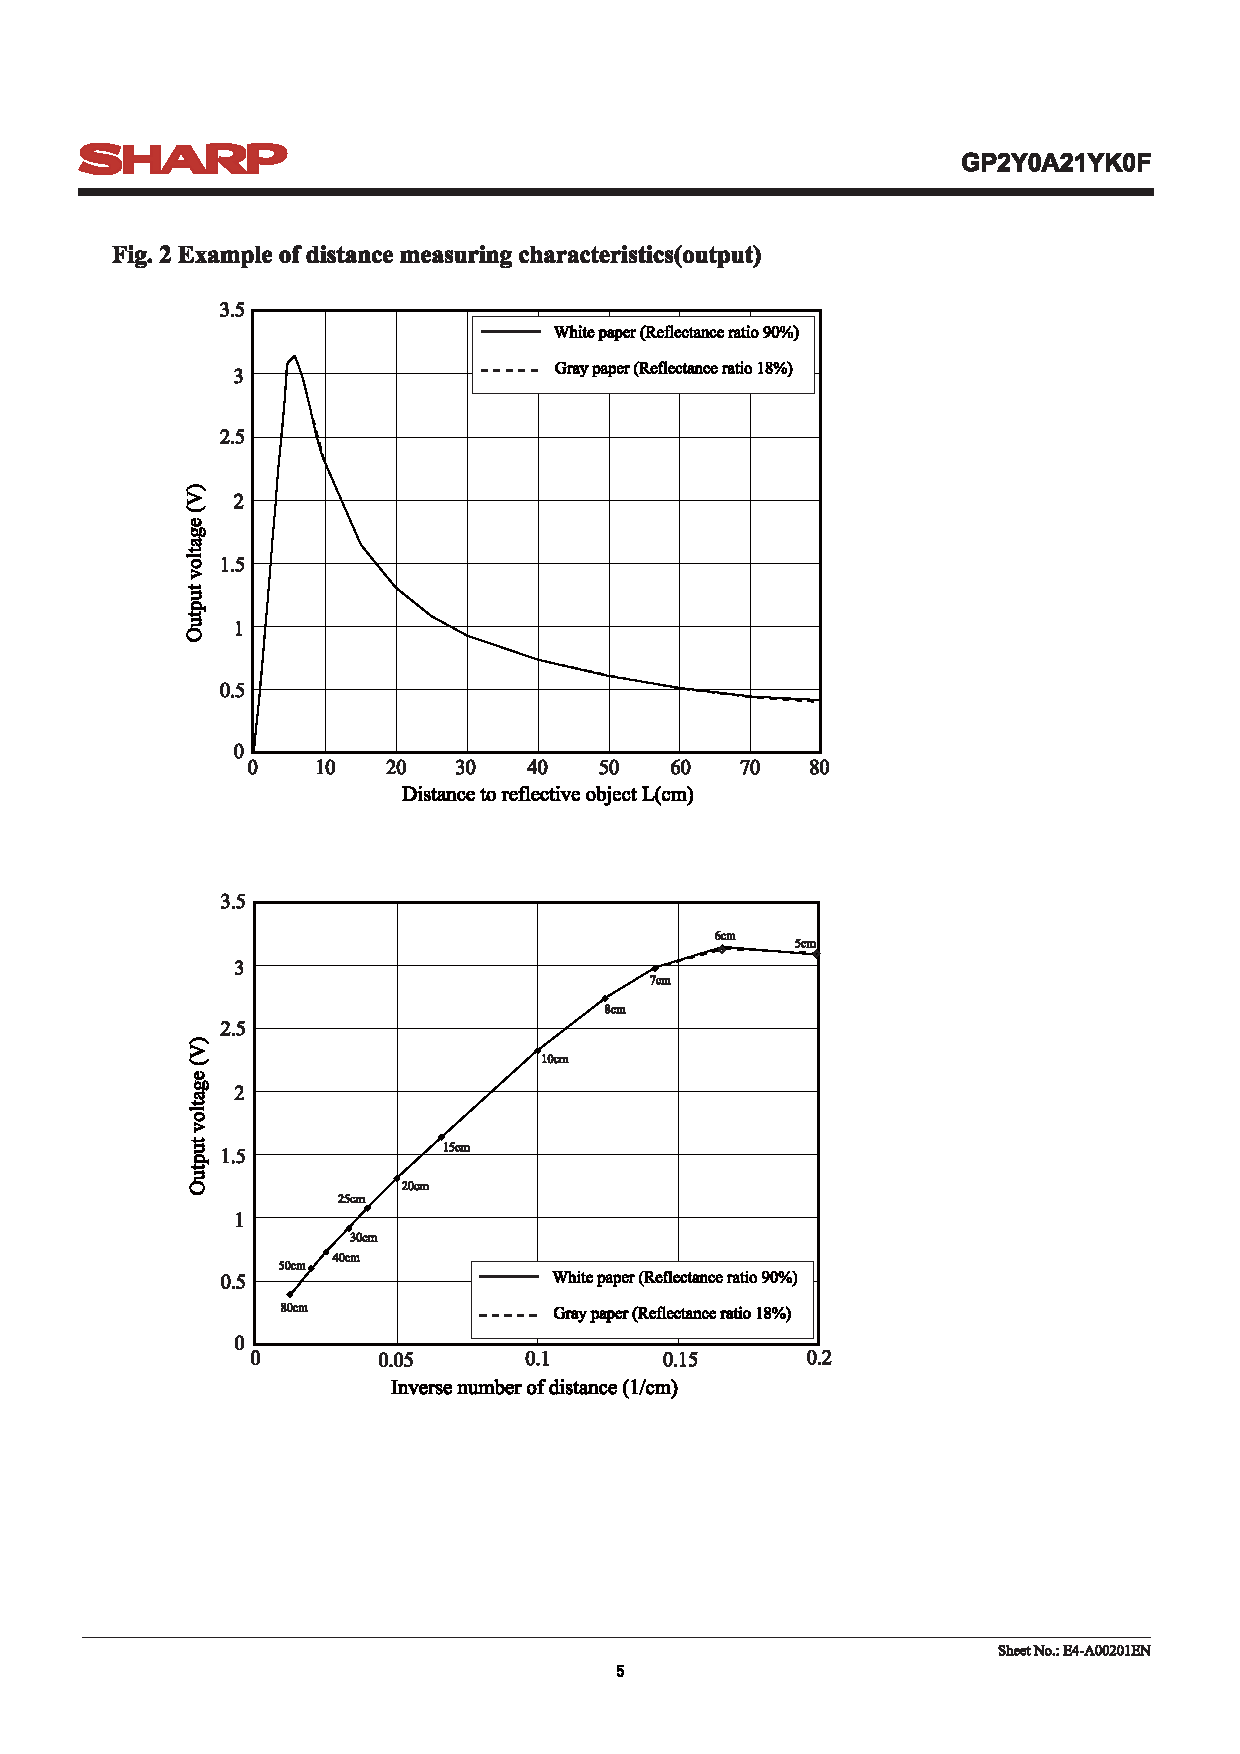
\includegraphics[trim =
%		{3cm 15.8cm 6.5cm 4.8cm}, clip,scale=1]{Figuras/IR_Datasheet_Figure}};
		
%	\node[fill,circle,inner sep=0.1pt, color = red] at (1.29,1.161) {};
%	\node[fill,circle,inner sep=0.1pt, color = red] at (2.525,2.235) {};
	
%	\node[fill,circle,inner sep=0.1pt, color = red] at (1.83,7.75) {};
	
	
%	\node[inner sep = 0 pt, outer sep = 0 pt] (origin) at (1.3,1.15) {};
%	\node[inner sep = 0 pt, outer sep = 0 pt] (teste2) at (2.55,2.25) {};
%	
%	\node[inner sep = 0 pt, outer sep = 0 pt] (P1) at (1.85,7.85) {};
	
	%\draw[-, color = red] (origin) -- (teste2);
	%\draw[-, color = red] (origin) -- (P1);
	
	%\node[] at (0,0) {};
	%\coordinate[] (teste1) {};
	%\coordinate[] (teste2) {};
	
	%\draw[-, color = red] (-18,2) -- (-7,3);
	
%	\end{tikzpicture}


	\textbf{Fonte: \citeonline{datasheet:SensorIR}}
\end{figure}
	\onslide<2>
		\begin{exampleblock}{Parâmetros}
			\begin{itemize}
			  \item Sensor IR: intervalo entre 10 e 80cm.
			  \item L = 18cm.
			  \item R = 3.4cm.
			\end{itemize}	
		\end{exampleblock}	
	\onslide<3>
		\vspace{-3.2cm}
		\begin{exampleblock}{Equação para distâncias do sensor IR}
			\begin{equation}
				\begin{split}
					d(v) = 2.7802212625 v^6 -35.1150300110 v^5 + 179.6031433005 v^4 \\
					-477.9449116299 v^3 + 706.3400747125 v^2 -569.7367375002 v \\
					+ 221.2678651473
				\end{split}
			\end{equation}
		\end{exampleblock}
\end{frame}

\begin{frame}
	\frametitle{Montagem Física}
	\begin{figure}[h]
\centering
\caption{Materiais e robô após montagem}
\label{fig:RoboReal}
	\begin{subfigure}[b]{0.49\textwidth}%
		\centering
		% fbox{}
		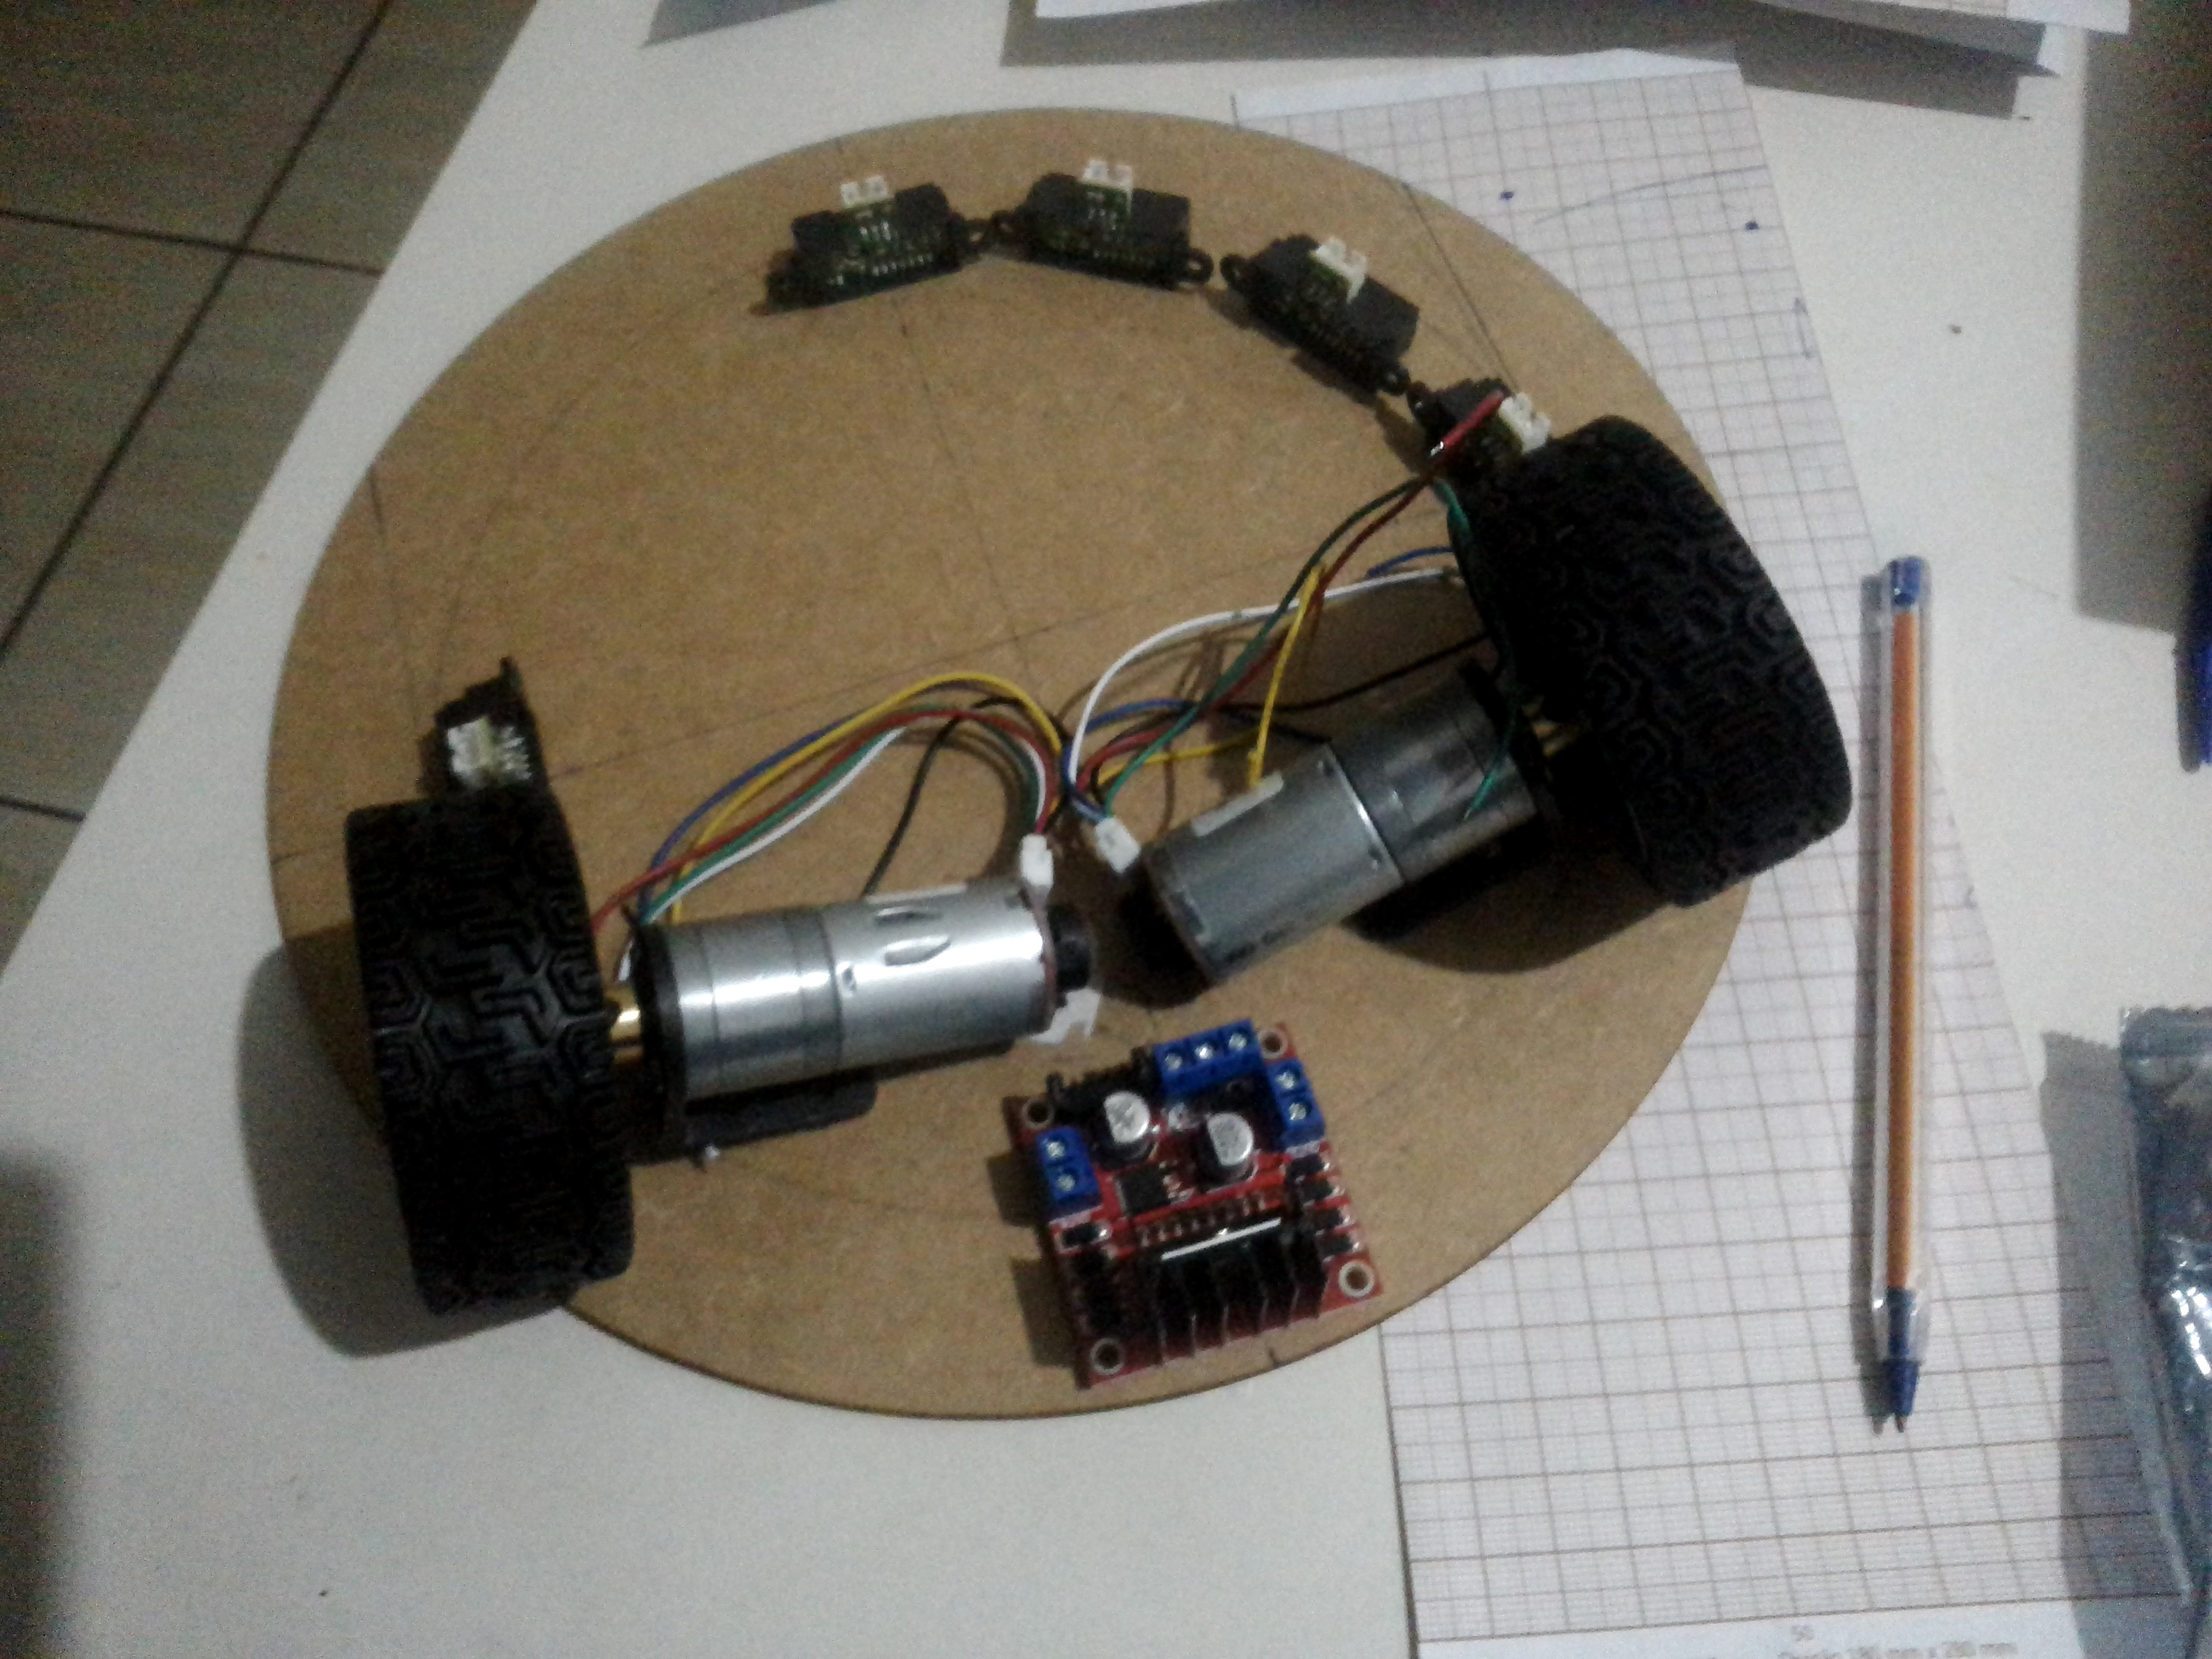
\includegraphics[trim= 0cm 0cm 0cm 0cm,clip,
scale=0.07]{Figuras/Robo1}
		\subcaption{Materiais do robô}
	  	%\label{fig:test1}
	\end{subfigure}
	~
	\begin{subfigure}[b]{0.49\textwidth}%
		\centering
		% fbox{}
		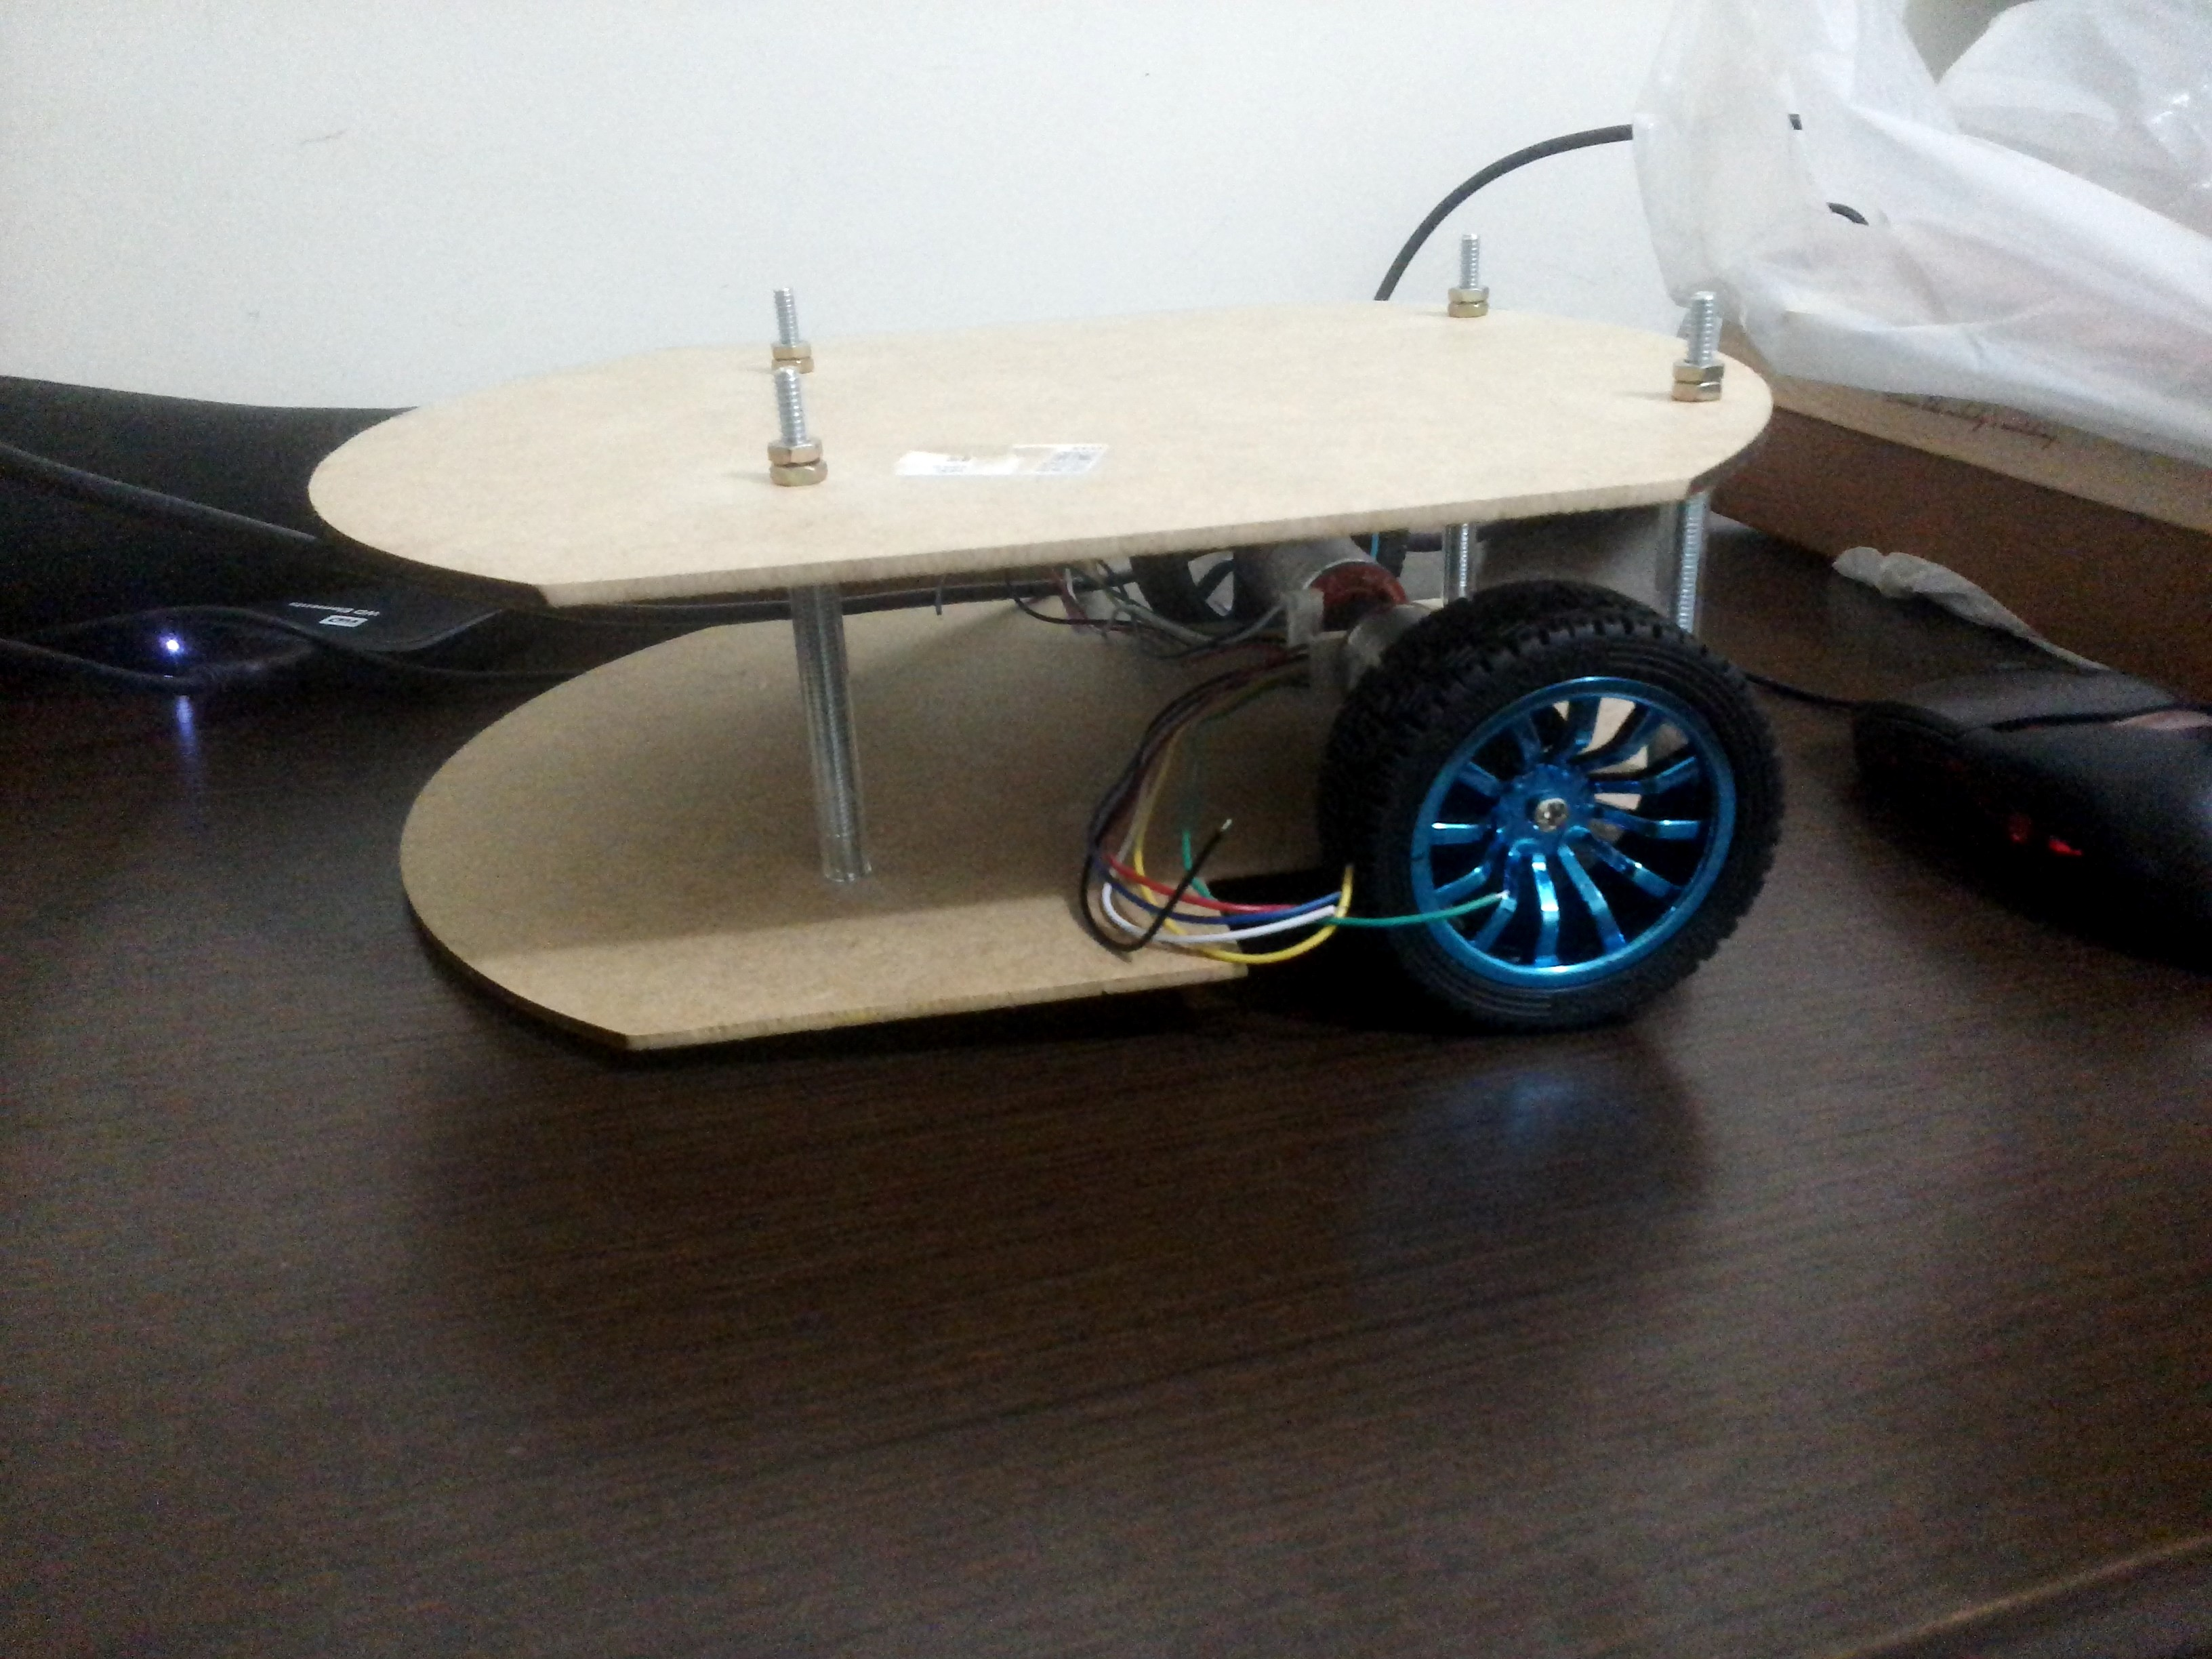
\includegraphics[trim={0cm 0cm 0cm 0cm},clip,
scale=0.07]{Figuras/Robo2}
		\subcaption{Robô montado}
	  	%\label{fig:test2}
	\end{subfigure}
	
	\textbf{Fonte: autoria própria}
\end{figure}
\end{frame}

\begin{frame}
	\begin{figure}[!ht]
\centering
	\begin{subfigure}[b]{0.49\textwidth}%
		\centering
		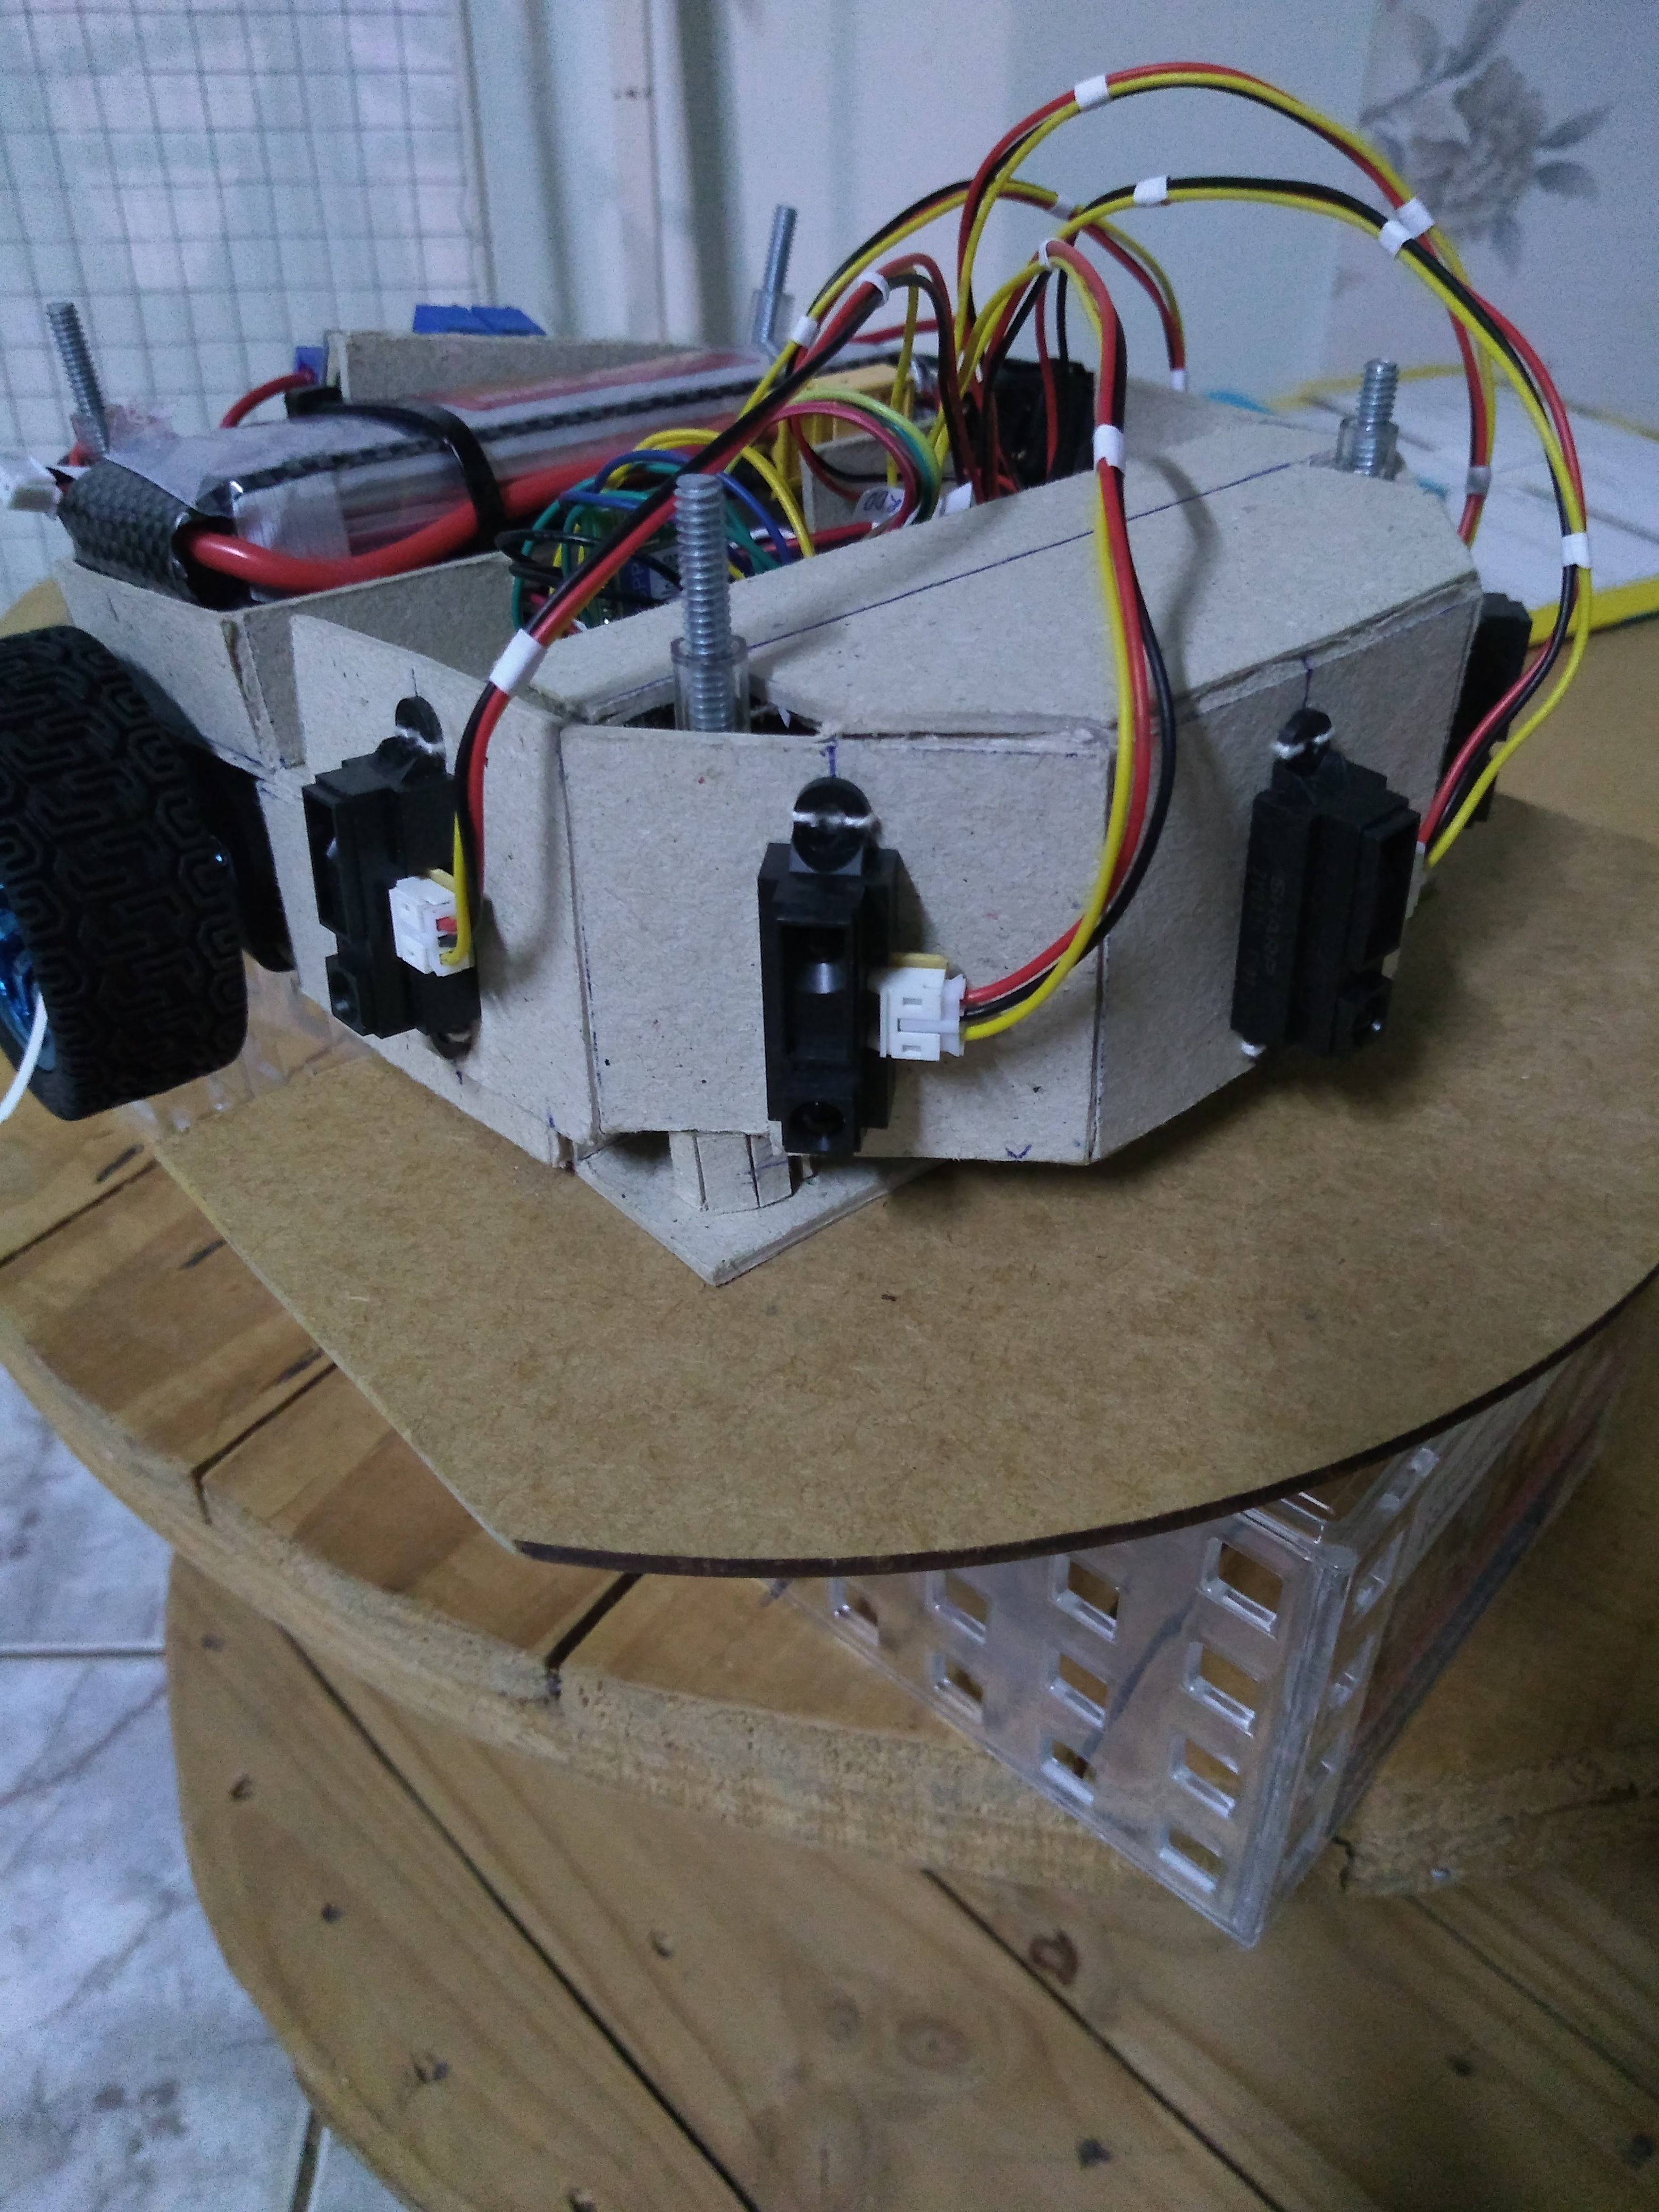
\includegraphics[trim={0cm 35cm 0cm 0cm}, clip, 
		scale=0.055]{Figuras/RoboMontagem5}%
		\subcaption{Posição dos parafusos de rosca}%
	\end{subfigure}%
	~
	\begin{subfigure}[b]{0.49\textwidth}%
		\centering
		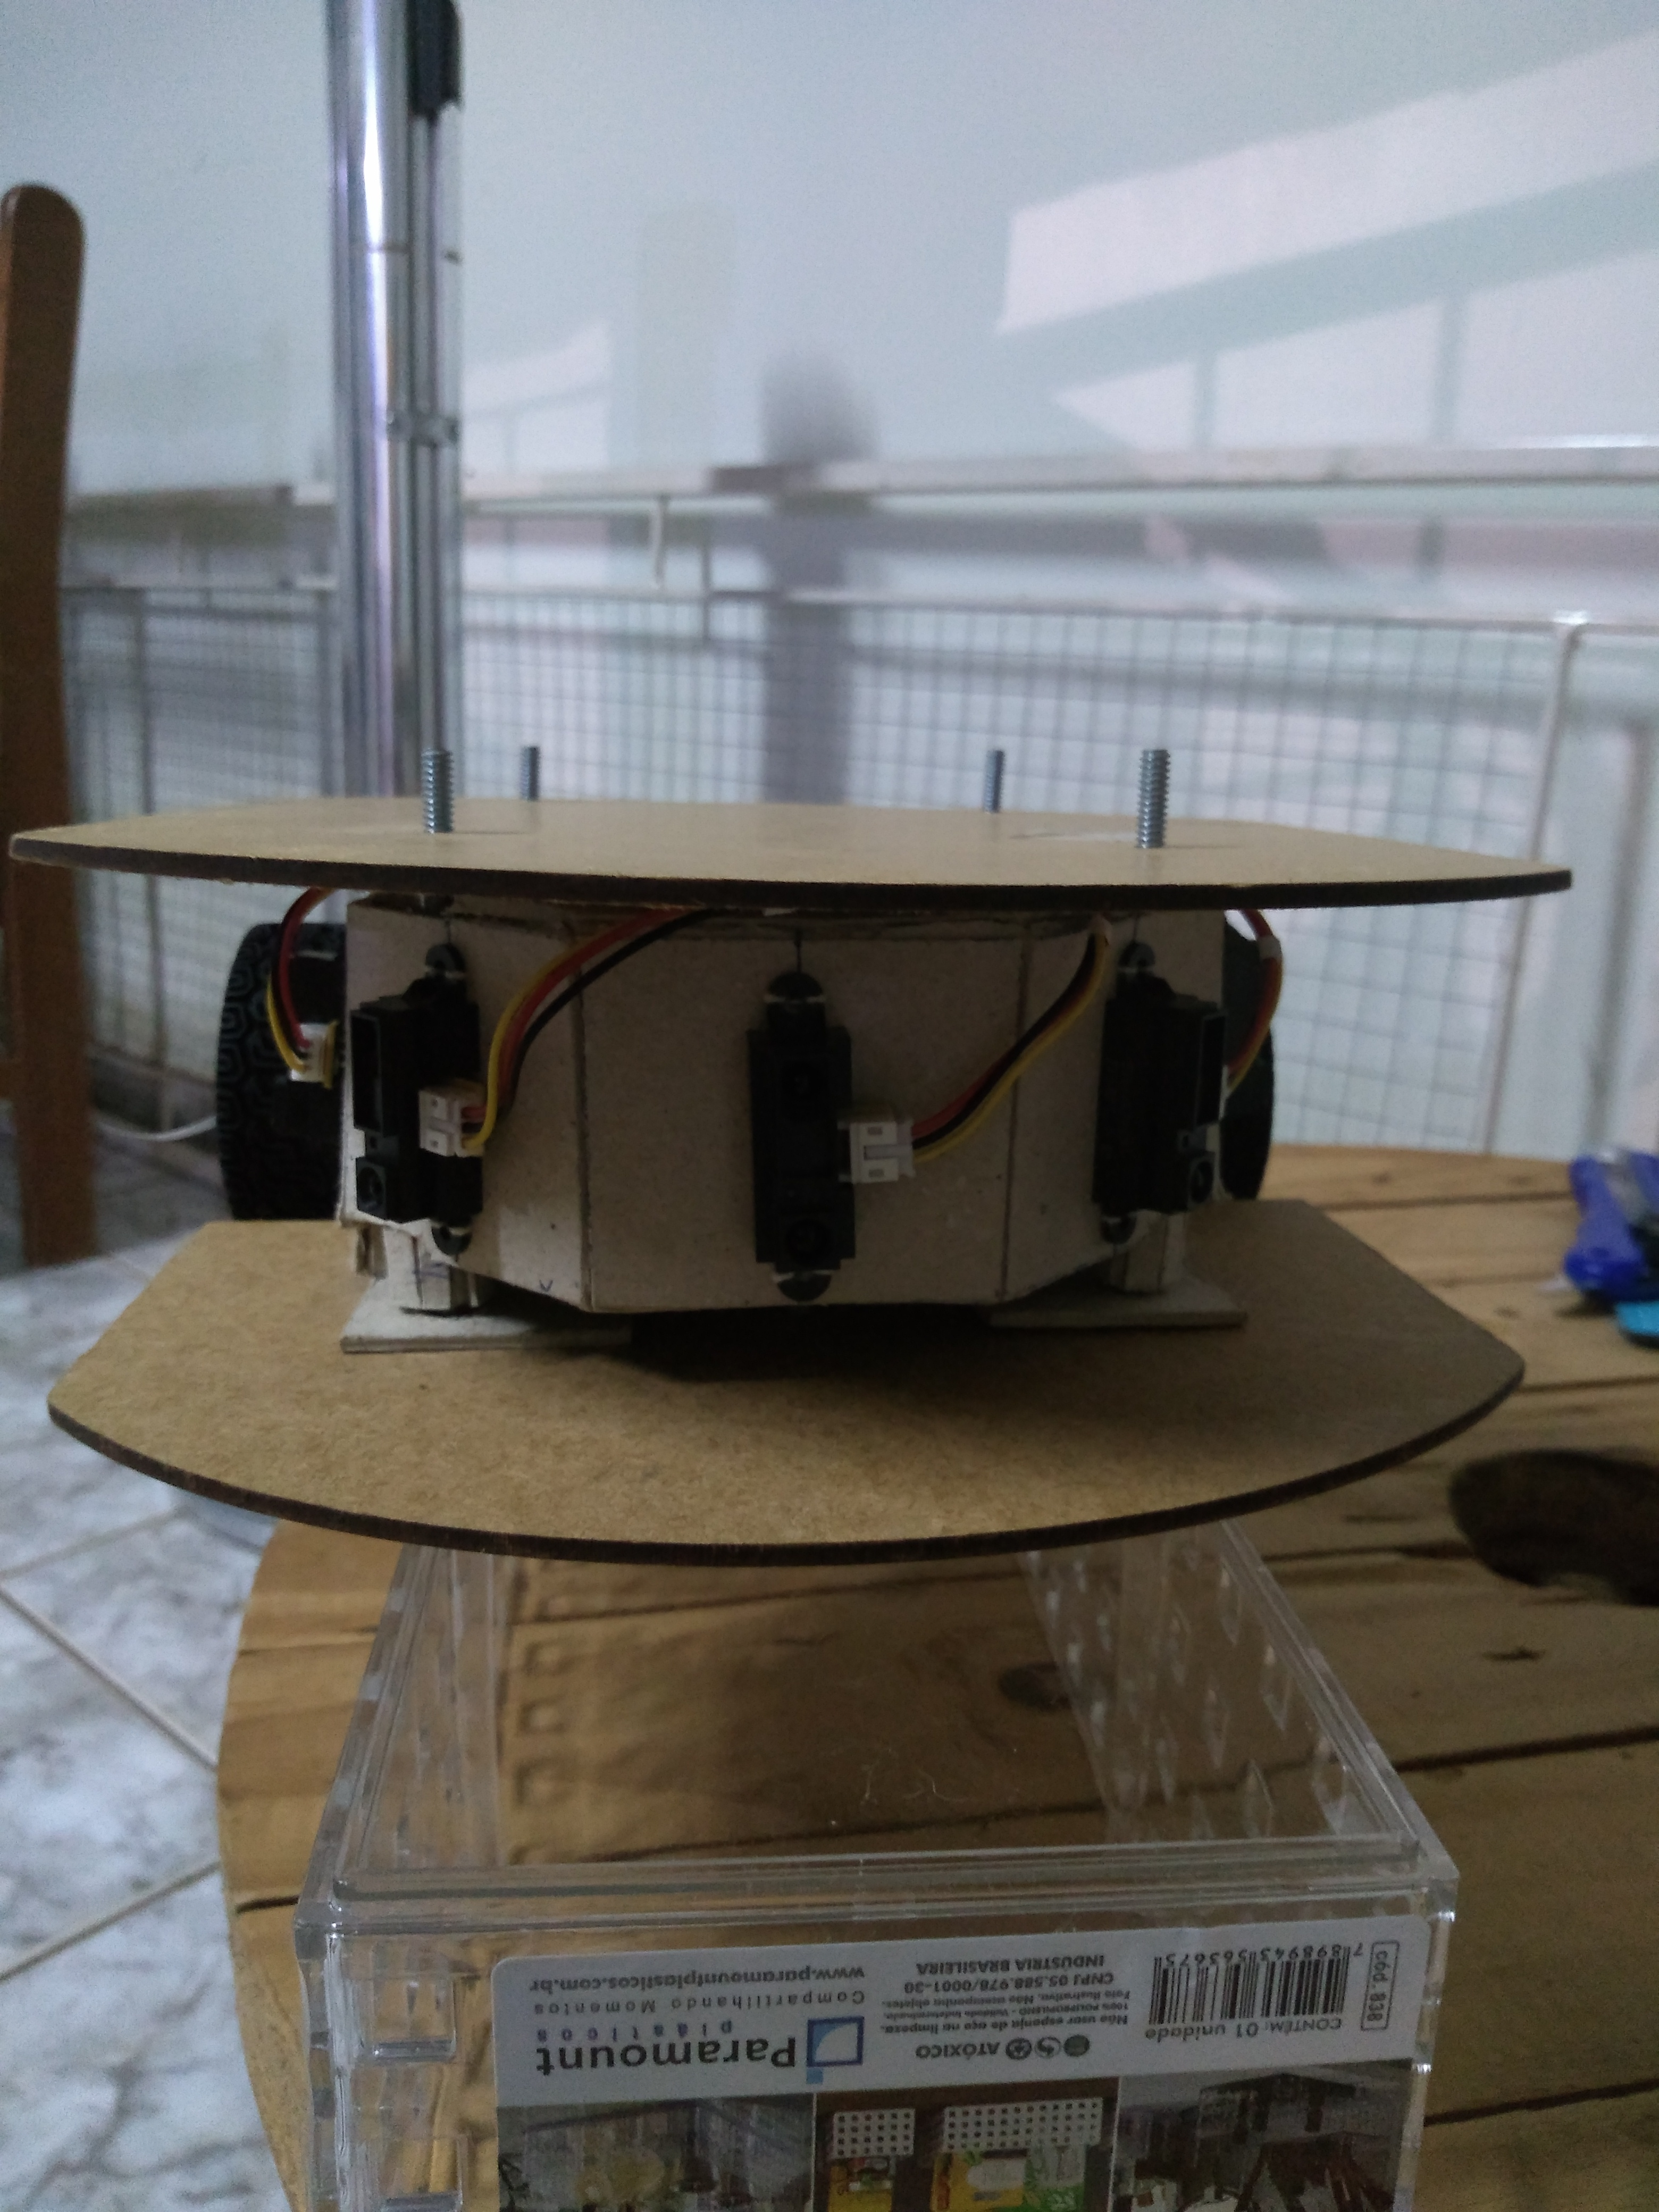
\includegraphics[trim={0cm 12.5cm 0cm 22.5cm}, clip, 
		scale=0.055]{Figuras/RoboMontagem6}%
		\subcaption{Robô montado}%
	\end{subfigure}%
\end{figure}
\end{frame}

\begin{frame}
	\frametitle{Curva para motores}
	\begin{figure}[!ht]
\centering
\caption{Curva do motor sem carga}
		\centering
		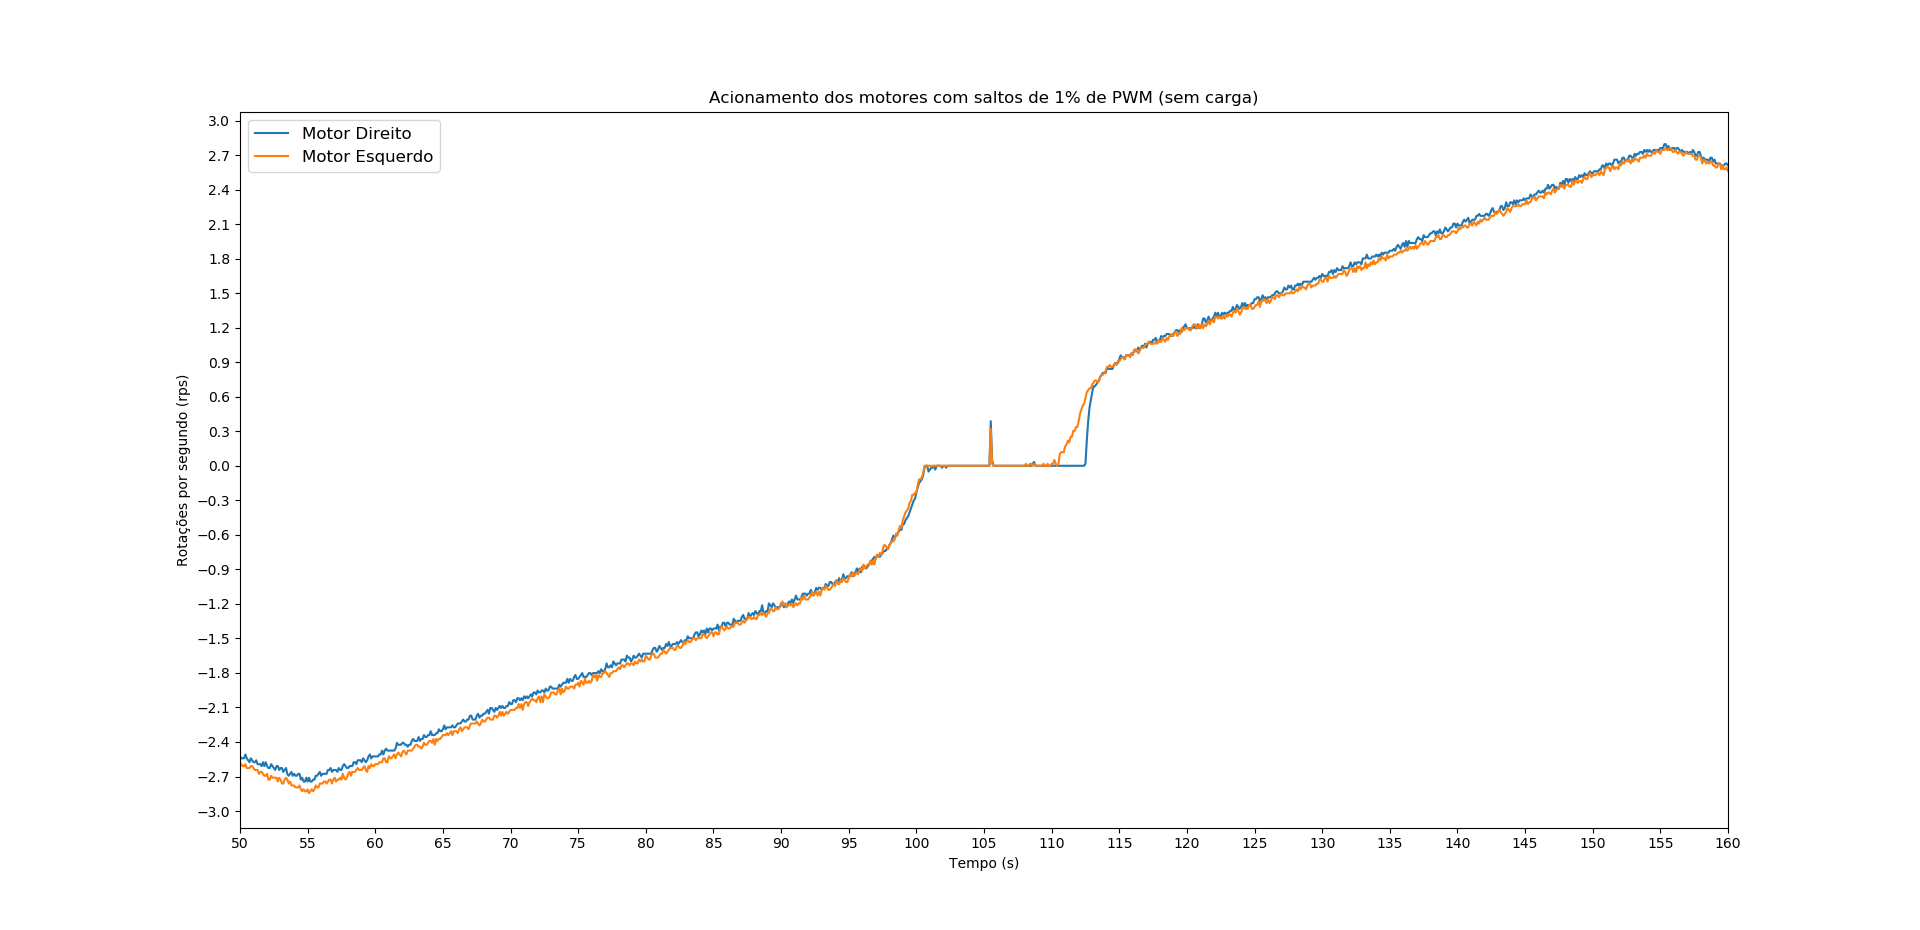
\includegraphics[trim={5cm 1cm 5cm 2cm},clip,
scale=0.25]{Figuras/Acionamento_Sem_Carga_rps}
\end{figure}
\end{frame}

\begin{frame}
	\begin{figure}[!ht]
\centering
\caption{Curva do motor com carga}
		\centering
		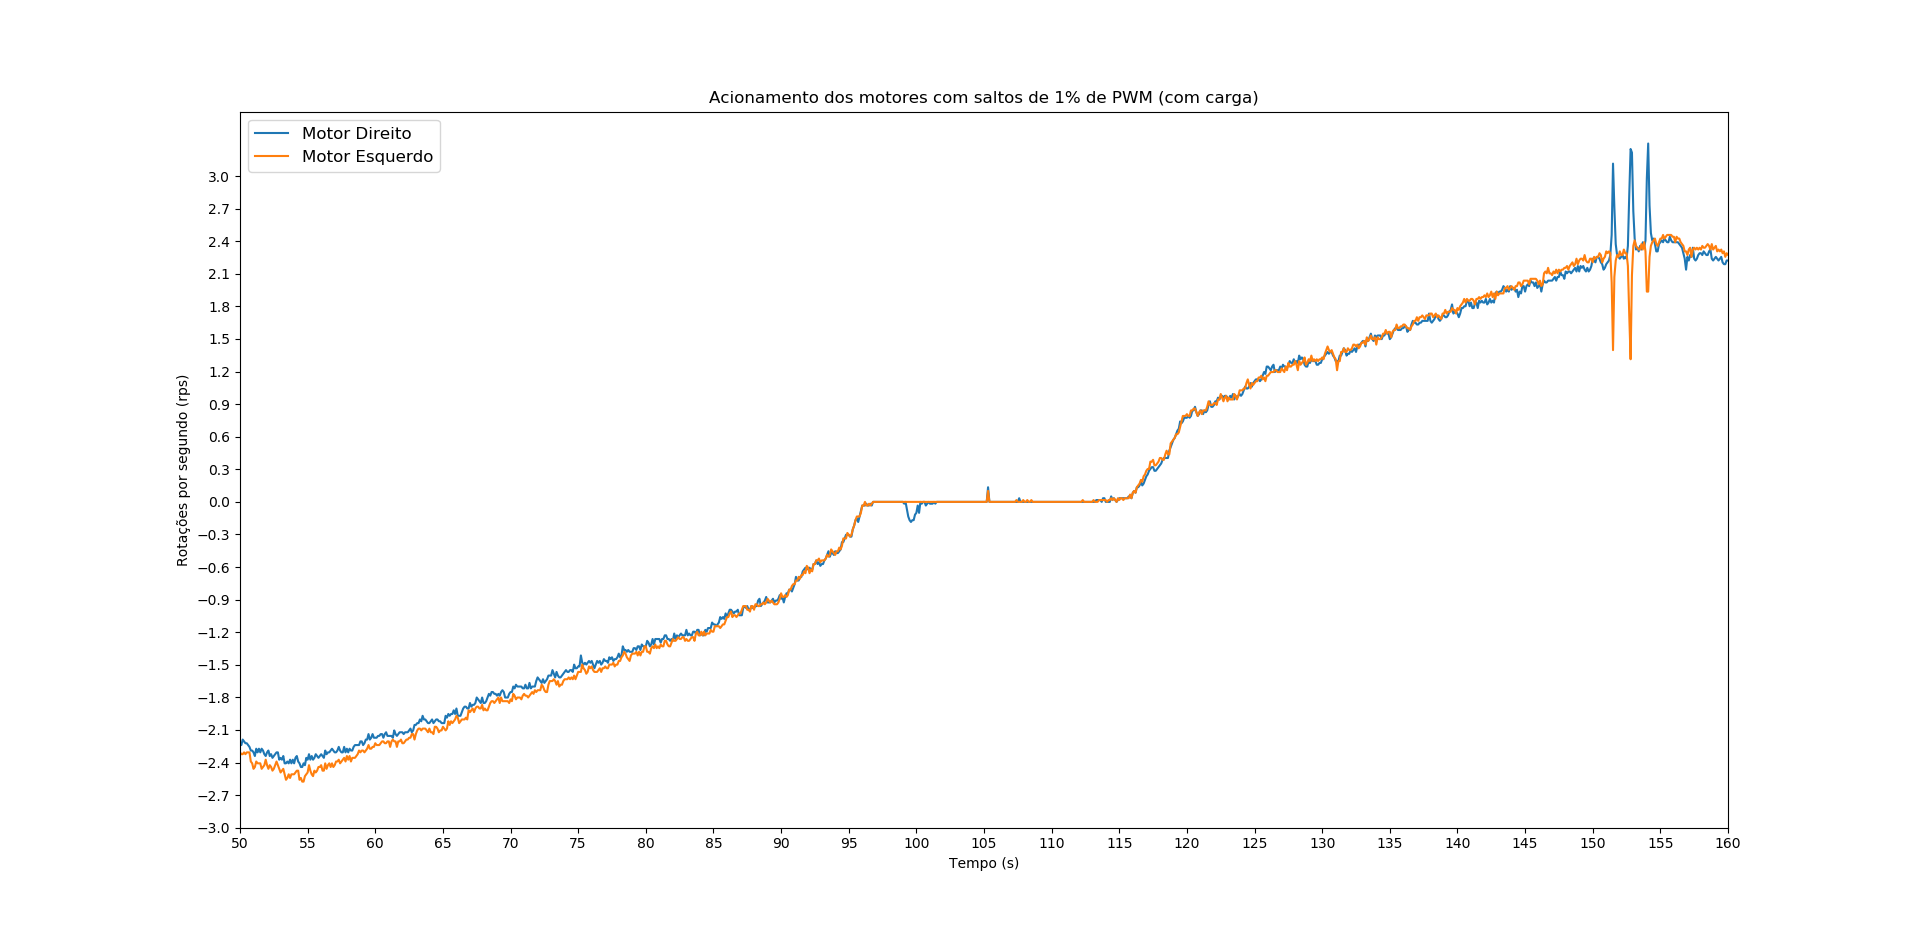
\includegraphics[trim={5cm 1cm 5cm 2cm},clip,
scale=0.25]{Figuras/Acionamento_Com_Carga_rps}
\end{figure}
\end{frame}

\begin{frame}
	\begin{figure}[!ht]
\centering
\caption{Regressão Linear para a curva do motor}
		\centering
		% fbox{}
		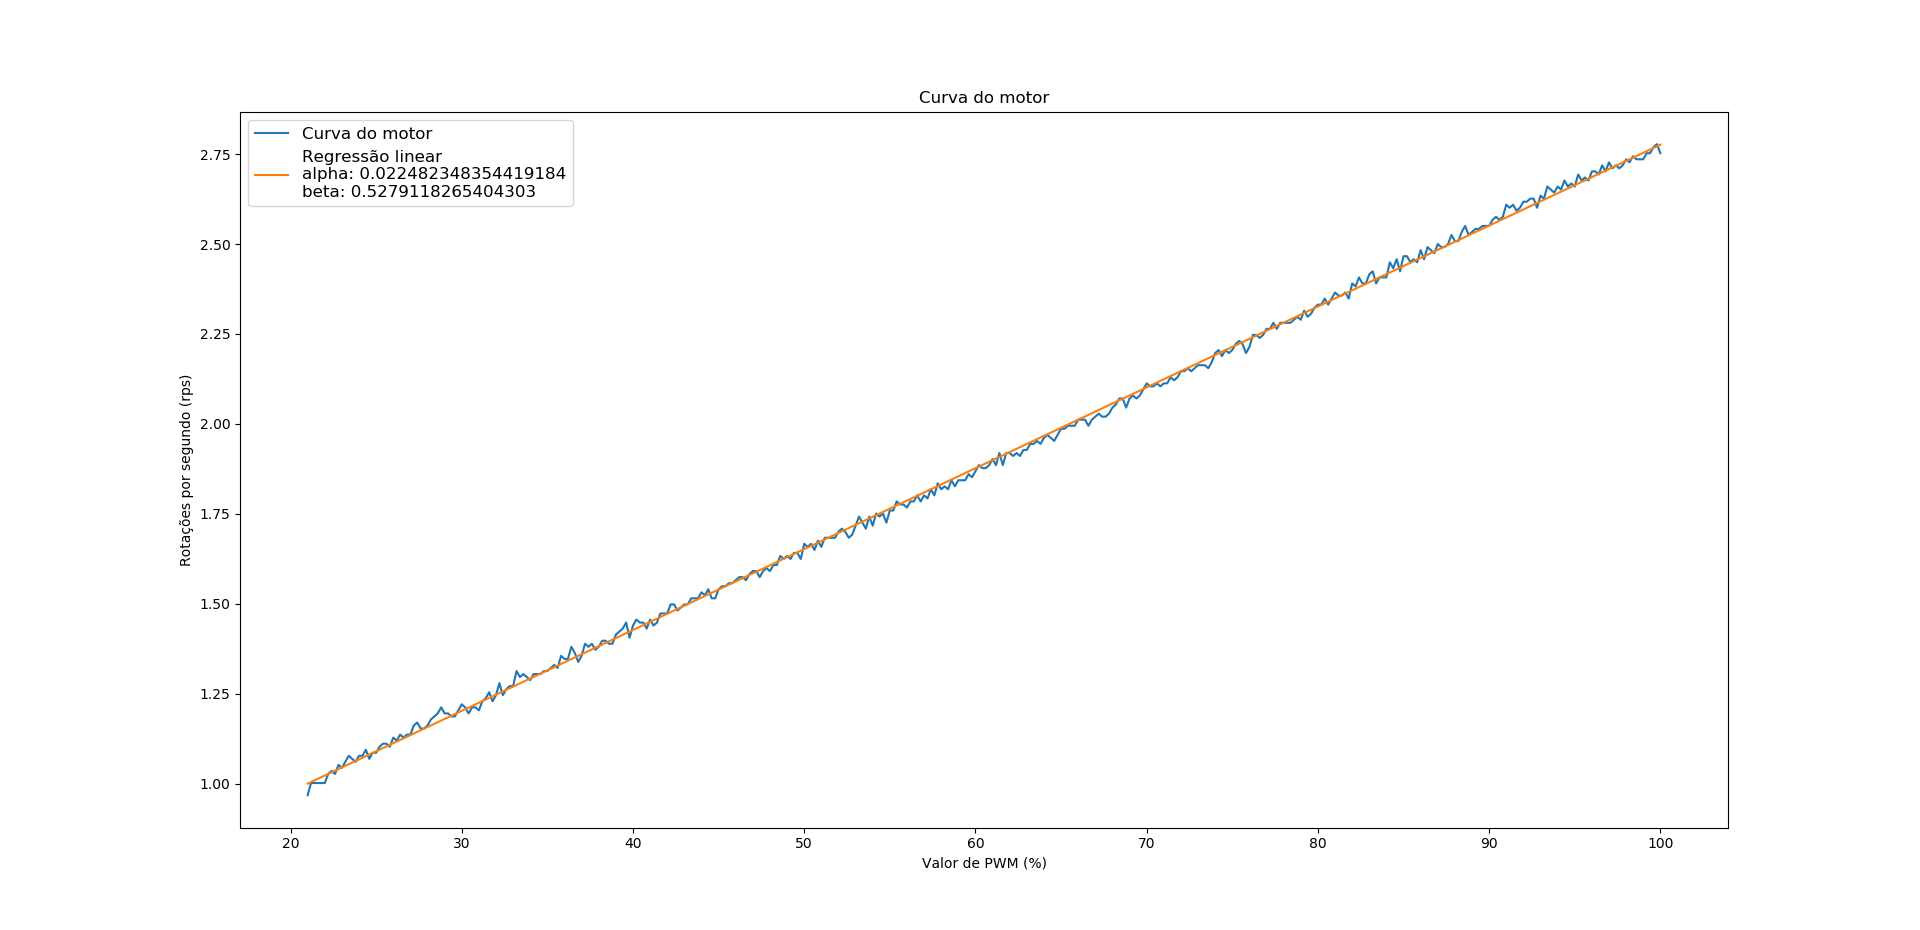
\includegraphics[trim={5cm 1cm 5cm 2cm},clip,
scale=0.25]{Figuras/Curva_Do_Motor_rps}
\end{figure}
\end{frame}
	
%%%%%%%%%%%%%%%%%%%%%%%%%%%%%
\begin{frame}
	\frametitle{Desenvolvimento}
	\begin{block}{Controlador Híbrido}
		Implementa arbitragem de comportamentos.
	\end{block}
	
	\begin{exampleblock}{Controlador Fuzzy}
		Implementa fusão de comportamentos.
	\end{exampleblock}
\end{frame}

\begin{frame}
	\frametitle{Controlador Híbrido}
	\begin{exampleblock}{Controlador PID}
		\begin{equation}
			\omega = K_p \epsilon(k) + K_i \sum_0^k \epsilon(k) T + k_d \frac{\epsilon(k) - \epsilon(k-1)}{T}
		\end{equation}
	\end{exampleblock}
	
	\onslide<2>
	\begin{block}{Considerações}
		\begin{itemize}
		  \item Velocidade angular tem prioridade sobre velocidade linear.
		  \item É necessário sacrificar velocidade linear em caso de saturação.
		\end{itemize}
	\end{block}
\end{frame}
	
\begin{frame}
	\begin{algorithm}[H]
		\algsetup{linenosize=\tiny}
		\scriptsize
		\caption{Uniciclo para Acionamento Diferencial priorizando $\omega$}
		\begin{algorithmic}[1]
			\onslide<1>
			\REQUIRE $v, \omega$
			\ENSURE $\omega_l, \omega_r$
			
			\IF{$v > 0$}
				\STATE $vlim \leftarrow max(min(abs(v), R \cdot VEL\_MAX), R \cdot VEL\_MIN)$
				\STATE $wlim \leftarrow max(min(abs(\omega), (R/L) \cdot (VEL\_MAX - VEL\_MIN)), 0)$
				
				\STATE $w_{l,lim}, w_{r,lim} \leftarrow uniToDiff(vlim, wlim)$
				
				\STATE $ velocidadeMaior \leftarrow max(w_{l,lim}, w_{r,lim})$
				\STATE $ velocidadeMenor \leftarrow min(w_{l,lim}, w_{r,lim})$
			
				\IF{$velocidadeMaior > VEL\_MAX$}
					\STATE $w_{l,lim} \leftarrow w_{l,lim} - (velocidadeMaior - VEL\_MAX)$
					\STATE $w_{r,lim} \leftarrow w_{r,lim} - (velocidadeMaior - VEL\_MAX)$
				\ELSIF{$velocidadeMenor < VEL\_MIN$}
					\STATE $w_{l,lim} \leftarrow w_{l,lim} + (VEL\_MIN - velocidadeMenor)$
					\STATE $w_{r,lim} \leftarrow w_{r,lim} + (VEL\_MIN - velocidadeMenor)$
				\ENDIF
				
				\IF{$v \geq 0$}
					\STATE $vlim \leftarrow 1$
				\ELSE
					\STATE $vlim \leftarrow -1$
				\ENDIF
				
				\onslide<2>
				\vspace{-6.5cm}
				\IF{$\omega \geq 0$}
					\STATE $wlim \leftarrow 1$
				\ELSE
					\STATE $wlim \leftarrow -1$
				\ENDIF
					
				\STATE $v,\omega \leftarrow diffToUni(w_{l,lim},w_{r,lim})$
				\STATE $v \leftarrow v \cdot vlim$
				\STATE $\omega \leftarrow \omega \cdot wlim$
			\ELSE
				\IF{$abs(\omega) > (R/L) \cdot 2 \cdot VEL\_MIN$}
					\IF{$\omega \geq 0$}
						\STATE $\omega \leftarrow max(min(abs(\omega),(R/L) \cdot 2 \cdot VEL\_MAX),(R/L) \cdot 2 \cdot VEL\_MIN)$ 
					\ELSE
						\STATE $\omega \leftarrow -max(min(abs(\omega),(R/L) \cdot 2 \cdot VEL\_MAX),(R/L) \cdot 2 \cdot VEL\_MIN)$
					\ENDIF
				\ELSE
					\STATE $\omega \leftarrow 0$
				\ENDIF
			\ENDIF
				
			\STATE $\omega_l, \omega_r \leftarrow uniToDiff(v,\omega)$
		\end{algorithmic}
	\end{algorithm}
\end{frame}

\begin{frame}
	\frametitle{Comportamento Ir Para Objetivo (IPO)}
	\newcommand{\meuRoboLindaoCompIPO}{
	\begin{tikzpicture}[scale = 1.5]%
		\coordsystwo{I}
		\begin{scope}[shift={(3, 0.9)}]
			\draw[->] (0.3,0) arc (0:30:0.3);
			\draw[-] (0,0) -- (0.4,0);
			\node at (0.5,0.1) {$\phi$};
			
			% Pr 
			\begin{scope}[scale = 0.5]
				\node[color = gray] at (0.1,-0.35) {$P_r$};
			\end{scope}
			\begin{scope}[rotate=30,scale=0.5]
				\begin{scope}[scale=0.9]
					\coordsystwo{R}
				\end{scope}
				\begin{scope}[shift={(0.25,0)},rotate = -90]
					\RoboDiffClean
				\end{scope}
			\end{scope}	
		\end{scope}
		
		% Coord objetivo
		\begin{scope}[shift={(4, 3)}]
			\filldraw (0,0) circle (1pt);
			% Po
			\begin{scope}[scale = 0.5]
				\node[color = gray] at (0.2,-0.45) {$P_o$};
			\end{scope}
		\end{scope}
		
		% retas
		\node[inner sep = 3pt] (P1) at (4,3) {};
		\node[inner sep = 3pt] (P2) at (3,0.9) {};
		
		\draw[->] (0,0) -- (P1);
		\draw[->] (0,0) -- (P2);
		\draw[->] (P2) -- (P1);
		
		% angulo do objetivo
		\draw[->] (0.6,0) arc (0:37:0.6);
		\draw[-] (0,0) -- (0.4,0);
		\node at (0.8,0.4) {$\theta$};
	\end{tikzpicture}%
}%

\begin{figure}[ht]
	\centering%
	\caption{Comportamento Ir para Objetivo}%
	\meuRoboLindaoCompIPO
\end{figure}
\end{frame}

\begin{frame}
	\begin{exampleblock}{Equações para Comportamento IPO}
		\begin{equation}
			\mathbf{u_{ipo}} = P_o - P_r
		\end{equation}
		
		\pause
		\begin{equation}
			e_\theta = atan2(u_{ipo,y}, u_{ipo,x}) - \phi
		\end{equation}
		
		\pause
		\begin{itemize}
		  \item $K_p = 4$
		  \pause
		  \item $K_i = 0,01$
		  \pause
		  \item $K_d = 0,01$
		\end{itemize}
	\end{exampleblock}
\end{frame}

\begin{frame}
	\frametitle{Comportamento Evitar Obstáculo (EO)}
	\newcommand{\meuRoboLindaoCompEO}{

	\begin{scope}[shift={(0,0.3)}]
		% Pr 
		\begin{scope}[shift={(0,-0.3)}, scale = 0.5]
			\node[color = gray] at (0.1,-0.35) {$P_r$};
		\end{scope}
		\begin{scope}[rotate=90,scale=0.5]
			\filldraw (0,0) circle (0.5pt);
			\begin{scope}[shift={(0.25,0)},rotate = -90]
				\RoboDiffClean
			\end{scope}
		\end{scope}
	\end{scope}
		
	% Obstáculo
	\begin{scope}[shift={(2,0)}]
		\obstaculo{3}
	\end{scope}
}%

\newcommand{\obstaculo}[1]{
	\node[inner sep = 0pt] (P1) at (0,0) {};
	\node[inner sep = 0pt] (P2) at (0.5,0) {};
	\node[inner sep = 0pt] (P3) at (0.5,#1) {};
	\node[inner sep = 0pt] (P4) at (0,#1) {};
	\draw (P1) -- (P2);
	\draw (P2) -- (P3);
	\draw (P3) -- (P4);
	\draw (P4) -- (P1);
}

\newcommand{\sensorVisaoTriangular}[1]{
	\draw (0,0) -- (-0.1,#1);
	\draw (0,0) -- (0.1,#1);
	\draw (-0.1,#1) -- (0.1,#1);
}

\newcommand{\sensorVisaoVetor}[1]{
	\draw[->] (0,0) -- (0,#1);
}

\newcommand{\desenharSensoresTriangulo}{
	\node[color = gray] at (-2.58,0.6) {$d_1$};
	\node[color = gray] at (-1.82,2.41) {$d_2$};
	\node[color = gray] at (0,3.07) {$d_3$};
	\node[color = gray] at (1.82,2.41) {$d_4$};
	\node[color = gray] at (2.24,0.6) {$d_5$};
	
	\begin{scope}[shift={(0.38,0.6)},rotate=-90]
		\sensorVisaoTriangular{2-0.38}
	\end{scope}
	\begin{scope}[shift={(-0.38,0.6)},rotate=90]
		\sensorVisaoTriangular{2}
	\end{scope}
	\begin{scope}[shift={(0.28,0.77)},rotate=-45]
		\sensorVisaoTriangular{2}
	\end{scope}
	\begin{scope}[shift={(-0.28,0.77)},rotate=45]
		\sensorVisaoTriangular{2}
	\end{scope}	
	\begin{scope}[shift={(0,0.87)},rotate=0]
		\sensorVisaoTriangular{2}
	\end{scope}
}

\newcommand{\desenharSensoresVetores}{
	\node[color = gray] at (-2.58,0.6) {$v_1$};
	\node[color = gray] at (-1.82,2.41) {$v_2$};
	\node[color = gray] at (0,3.07) {$v_3$};
	\node[color = gray] at (1.82,2.41) {$v_4$};
	\node[color = gray] at (2.24,0.6) {$v_5$};
	
	\begin{scope}[shift={(0.38,0.6)},rotate=-90]
		\sensorVisaoVetor{2-0.38}
	\end{scope}
	\begin{scope}[shift={(-0.38,0.6)},rotate=90]
		\sensorVisaoVetor{2}
	\end{scope}
	\begin{scope}[shift={(0.28,0.77)},rotate=-45]
		\sensorVisaoVetor{2}
	\end{scope}
	\begin{scope}[shift={(-0.28,0.77)},rotate=45]
		\sensorVisaoVetor{2}
	\end{scope}	
	\begin{scope}[shift={(0,0.87)},rotate=0]
		\sensorVisaoVetor{2}
	\end{scope}
}


\begin{figure}[ht]
	\centering%
	\begin{subfigure}[t]{0.5\textwidth}%
		\centering%
			
		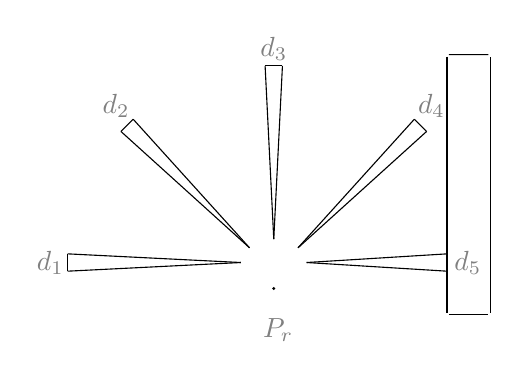
\begin{tikzpicture}[scale = 1.1]%
			\meuRoboLindaoCompEO
			\desenharSensoresTriangulo
		\end{tikzpicture}%
		
		\caption{Sensores infravermelho}%
	\end{subfigure}%
	~
	\begin{subfigure}[t]{0.5\textwidth}%
		\centering%
		
		\begin{tikzpicture}[scale = 1.1]%
			\meuRoboLindaoCompEO
			\desenharSensoresVetores
		\end{tikzpicture}%
			
		\caption{Vetores utilizados}%
	\end{subfigure}%
\end{figure}
\end{frame}

\begin{frame}
	\begin{block}{Conversão de sistemas de coordenadas}
		\begin{equation}
			\mleft[ 
			\begin{array}{c c}
				x \\ y
			\end{array}
			\mright]_i^R = \mleft[
			\begin{matrix}
		  		\cos{\theta_i} & -\sin{\theta_i} \\
		  		\sin{\theta_i} & \cos{\theta_i} \\
			\end{matrix}
			\mright] \mleft[ 
			\begin{array}{c c}
				d_i \\ 0
			\end{array}
			\mright] + \mleft[ 
			\begin{array}{c c}
				o_x \\ o_y
			\end{array}
			\mright]_i^R
		\end{equation}
	\end{block}
	
	\pause
	\begin{exampleblock}{Combinação Linear}
		\begin{equation}
			\mathbf{u_{eo2}} = k_1 \mathbf{v_1} + k_2 \mathbf{v_2} + k_3 \mathbf{v_3} + 
			k_4 \mathbf{v_4} + k_5 \mathbf{v_5}
		\end{equation}
	\end{exampleblock}
	
	\pause
	\begin{block}{Equilíbrio}
		\begin{equation}
			\mathbf{u_{eo1}} = k_1 \mathbf{v_1} + k_2 \mathbf{v_2} + k_3 \mathbf{v_3} + 
			k_4 \mathbf{v_4} + k_5 \mathbf{v_5} + \mathbf{v_{eq}}
		\end{equation}
	\end{block}
\end{frame}

\begin{frame}
	\begin{block}{Parâmetros}
		\begin{itemize}
		  \item Constantes $k_i$:
			  \subitem{$k_1 = 0,7$}
			  \subitem{$k_2 = 2$}
			  \subitem{$k_3 = 1,2$}
			  \subitem{$k_4 = 2$} 
			  \subitem{$k_5 = 0,7$}
		  \pause
		  \item $\mathbf{v_{eq}} = [-240 \ 0]^T$
		  \pause
		  \item $D_{insegura} = 25$
		\end{itemize}
	\end{block}
\end{frame}

\begin{frame}
	\begin{exampleblock}{Comportamento EO completo}
		\begin{equation}
			\mathbf{u_{eo}} = 
			\begin{cases}
				\mathbf{u_{eo1}} & \text{para} \ | \mathbf{v_3} | \geq D_{insegura} \\
				
				\mleft[
				\begin{matrix}
		  			\cos{(90)} & -\sin{(90)} \\
		  			\sin{(90)} & \cos{(90)} \\
				\end{matrix}
				\mright] \mathbf{u_{eo2}} & 				
				\begin{matrix*}[l]
		  			\text{para} \ | \mathbf{v_3} | < D_{insegura} \ \land \\
		  			k_1 \ (|\mathbf{v_5}| - |\mathbf{v_1}|) + k_2 \ (|\mathbf{v_4}| - |\mathbf{v_2}|)
					> 0 \\
				\end{matrix*} \\
				
				\mleft[
				\begin{matrix}
		  			\cos{(-90)} & -\sin{(-90)} \\
		  			\sin{(-90)} & \cos{(-90)} \\
				\end{matrix}
				\mright] \mathbf{u_{eo2}} & 
				\begin{matrix*}[l]
		  			\text{para} \ | \mathbf{v_3} | < D_{insegura} \ \land \\
		  			k_1 \ (|\mathbf{v_5}| - |\mathbf{v_1}|) + k_2 \ (|\mathbf{v_4}| - |\mathbf{v_2}|)
					\leq 0 \\
				\end{matrix*} \\
			\end{cases}
		\end{equation}
	\end{exampleblock}
\end{frame}

\begin{frame}
	\frametitle{Comportamento Mesclado IPO + EO}
	\begin{block}{Cálculo da recomendação}
		\begin{equation}
			\mathbf{u_{eo\_e\_ipo}} = k \ \hat{\mathbf{u}}_{ipo} + (1-k) \ \hat{\mathbf{u}}_{eo}
		\end{equation}
		
		\pause
		\begin{itemize}
		  \item $k = 0,3$
		\end{itemize}
	\end{block}
	
	\pause
	\begin{exampleblock}{IPO}
		\begin{equation}
			\mathbf{u_{ipo}} = P_o - P_r
		\end{equation}
	\end{exampleblock}
	
	\pause
	\begin{block}{EO}
		\begin{equation}
			\mathbf{u_{eo1}} = k_1 \mathbf{v_1} + k_2 \mathbf{v_2} + k_3 \mathbf{v_3} + 
			k_4 \mathbf{v_4} + k_5 \mathbf{v_5} + \mathbf{v_{eq}}
		\end{equation}
	\end{block}
\end{frame}

\begin{frame}
	\frametitle{O problema dos Mínimos Locais}
	\newcommand{\meuRoboLindaoCompMinimos}{
	\begin{scope}[shift={(0,0.3)}]
		% Pr 
		\begin{scope}[shift={(0,-0.3)}, scale = 0.5]
			\node[color = gray] at (0.1,-0.35) {$P_r$};
		\end{scope}
		\begin{scope}[rotate=90,scale=0.5]
			\filldraw (0,0) circle (0.5pt);
			\begin{scope}[shift={(0.25,0)},rotate = -90]
				\RoboDiffClean
			\end{scope}
		\end{scope}
	\end{scope}
}%

\newcommand{\obstaculoA}[2]{
	\node[inner sep = 0pt] (P1) at (#1,0) {};
	\node[inner sep = 0pt] (P2) at (\fpeval{#1+(#2/2)},\fpeval{#2*sqrt{2}/2}) {};
	\node[inner sep = 0pt] (P3) at (\fpeval{#1+((3*#2)/2)},\fpeval{#2*sqrt{2}/2}) {};
	\node[inner sep = 0pt] (P4) at (\fpeval{#1+2*#2},0) {};
	\node[inner sep = 0pt] (P5) at (\fpeval{#1+((3*#2)/2)},\fpeval{-(#2*sqrt{2}/2)}) {};
	\node[inner sep = 0pt] (P6) at (\fpeval{#1+(#2/2)},\fpeval{-(#2*sqrt{2}/2)}) {};
	
	\draw[color = darkgray] (P1) -- (P2);
	\draw[color = darkgray] (P2) -- (P3);
	\draw[color = darkgray] (P3) -- (P4);
	\draw[color = darkgray] (P4) -- (P5);
	\draw[color = darkgray] (P5) -- (P6);
	\draw[color = darkgray] (P6) -- (P1);
	
	\node[color = gray] at (#1+#2,-1.3) {Obstáculo 1};
}

\newcommand{\obstaculoB}[3]{
	\node[inner sep = 0pt] (P1) at (#1,#2) {};
	\node[inner sep = 0pt] (P2) at (#1,#2+0.5) {};
	\node[inner sep = 0pt] (P3) at (#1+#3+0.5,#2+0.5) {};
	\node[inner sep = 0pt] (P4) at (#1+#3+0.5,-#2-0.5) {};
	
	\node[inner sep = 0pt] (P5) at (#1,-#2-0.5) {};
	\node[inner sep = 0pt] (P6) at (#1,-#2) {};
	\node[inner sep = 0pt] (P7) at (#1+#3,-#2) {};
	\node[inner sep = 0pt] (P8) at (#1+#3,#2) {};
	
	\draw[color = darkgray] (P1) -- (P2);
	\draw[color = darkgray] (P2) -- (P3);
	\draw[color = darkgray] (P3) -- (P4);
	\draw[color = darkgray] (P4) -- (P5);
	\draw[color = darkgray] (P5) -- (P6);
	\draw[color = darkgray] (P6) -- (P7);
	\draw[color = darkgray] (P7) -- (P8);
	\draw[color = darkgray] (P8) -- (P1);
	
	\node[color = gray] at (#1+0.25+#3/2,-2.8) {Obstáculo 2};
}

\newcommand{\obstaculoC}[2]{
	\node[inner sep = 0pt] (P1) at (#1,#2+0.5) {};
	\node[inner sep = 0pt] (P2) at (#1+0.5,#2+0.5) {};
	\node[inner sep = 0pt] (P3) at (#1+0.5,-#2-0.5) {};
	\node[inner sep = 0pt] (P4) at (#1,-#2-0.5) {};
	
	\draw[color = darkgray] (P1) -- (P2);
	\draw[color = darkgray] (P2) -- (P3);
	\draw[color = darkgray] (P3) -- (P4);
	\draw[color = darkgray] (P4) -- (P1);
	
	\node[color = gray] at (#1+0.25,-2.8) {Obstáculo 3};
}

\begin{figure}[ht]
	\centering%
	
	\begin{tikzpicture}[scale = 1.1]%
		% Robô
		\begin{scope}[rotate=-90]
			\meuRoboLindaoCompMinimos
		\end{scope}
		\obstaculoA{2}{1.5}
		\obstaculoB{4}{2}{2}
		\obstaculoC{8}{2}
		
		\begin{scope}[shift={(10,0)}]
			\filldraw (0,0) circle (1.5pt);
			\node[color = gray] at (0,-0.35) {Objetivo};
		\end{scope}
	\end{tikzpicture}%
\end{figure}
\end{frame}

\begin{frame}
	\frametitle{Comportamento Seguir Parede}
	\newcommand{\parede}[2]{
	\node[inner sep = 0pt] (P1) at (0,0) {};
	\node[inner sep = 0pt] (P2) at (#2,0) {};
	\node[inner sep = 0pt] (P3) at (#2,0.5) {};
	\node[inner sep = 0pt] (P4) at (0.5,0.5) {};
	\node[inner sep = 0pt] (P5) at (0.5,#1) {};
	\node[inner sep = 0pt] (P6) at (0,#1) {};
	\draw[color = darkgray] (P1) -- (P2);
	\draw[color = darkgray] (P2) -- (P3);
	\draw[color = darkgray] (P3) -- (P4);
	\draw[color = darkgray] (P4) -- (P5);
	\draw[color = darkgray] (P5) -- (P6);
	\draw[color = darkgray] (P6) -- (P1);
}

\newcommand{\sensorVisaoVetorSp}[1]{
	\draw[->] (0,0) -- (0,#1);
}

\newcommand{\desenharSensoresTrianguloSPb}{
	\begin{scope}[shift={(0.38,0.6)},rotate=-90]
		\sensorVisaoTriangularSp{2-0.9}
	\end{scope}
	\begin{scope}[shift={(-0.38,0.6)},rotate=90]
		\sensorVisaoTriangularSp{2}
	\end{scope}
	\begin{scope}[shift={(0.28,0.77)},rotate=-45]
		\sensorVisaoTriangularSp{2-0.5}
	\end{scope}
	\begin{scope}[shift={(-0.28,0.77)},rotate=45]
		\sensorVisaoTriangularSp{2}
	\end{scope}	
	\begin{scope}[shift={(0,0.87)},rotate=0]
		\sensorVisaoTriangularSp{2-1}
	\end{scope}
}

\newcommand{\desenharLinhasParedeA}{
	\begin{scope}[shift={(-0.38,0.6)},rotate=90]
		\begin{scope}[shift={(0,2-1.3)}]
			\node[inner sep = 0pt] (P1) at (0,0) {};
		\end{scope}
	\end{scope}
	\begin{scope}[shift={(-0.28,0.77)},rotate=45]
		\begin{scope}[shift={(0,2)}]
			\node[inner sep = 0pt] (P2) at (0,0) {};
		\end{scope}
	\end{scope}
	
	\draw (P1) -- (P2);
}

\newcommand{\desenharLinhasParedeB}{
	\begin{scope}[shift={(0.38,0.6)},rotate=-90]
		\begin{scope}[shift={(0,2-0.9)}]
			\node[inner sep = 0pt] (P1) at (0,0) {};
		\end{scope}
	\end{scope}
	\begin{scope}[shift={(0,0.87)},rotate=0]
		\begin{scope}[shift={(0,2-1)}]
			\node[inner sep = 0pt] (P2) at (0,0) {};
		\end{scope}
	\end{scope}
	
	\draw (P1) -- (P2);
}

\begin{figure}[ht]
	\centering%
	\begin{subfigure}[t]{0.5\textwidth}%
		\centering%
		\begin{tikzpicture}[scale = 1.1]%
			% Obstáculo
			\parede{3}{2}
			% Robô
			\begin{scope}[shift={(-1.1,1.4)},rotate=180]
				\meuRoboLindaoCompSP
				\desenharSensoresTrianguloSPa
				\desenharLinhasParedeA
			\end{scope}
		\end{tikzpicture}%
		
		\caption{Parede subestimada}%
	\end{subfigure}%
	~
	\begin{subfigure}[t]{0.5\textwidth}%
		\centering%
		\begin{tikzpicture}[scale = 1.1]%
			% Obstáculo
			\begin{scope}[shift={(0,0)},xscale=-1,yscale=1]
				\parede{3}{4}
			\end{scope}
			% Robô
			\begin{scope}[shift={(-2.4,2)},rotate=-90]
				\meuRoboLindaoCompSP
				\desenharSensoresTrianguloSPb
				\desenharLinhasParedeB
			\end{scope}
		\end{tikzpicture}%
			
		\caption{Parede superestimada}%
	\end{subfigure}%
\end{figure}
\end{frame}

\begin{frame}
	\newcommand{\desenharLinhasParedeC}[2]{
	\begin{scope}[shift={(-0.38,0.6)},rotate=90]
		\begin{scope}[shift={(0,2-1.3)}]
			\node[inner sep = 0pt] (P1) at (0,0) {};
		\end{scope}
	\end{scope}
	\begin{scope}[shift={(-0.28,0.77)},rotate=45]
		\begin{scope}[shift={(0,2)}]
			\node[inner sep = 0pt] (P2) at (0,0) {};
		\end{scope}
	\end{scope}
	
	\draw (P1) -- (P2);
	
	% linhas continuacao:
	\def\UserVetAX{-1.08}
	\def\UserVetAY{0.6}
	
	\def\UserVetXNum{\fpeval{-0.28-sqrt(2)+1.08}}
	\def\UserVetYNum{\fpeval{0.77+sqrt(2)-0.6}}
	\def\UserVetMod{\fpeval{sqrt(\UserVetXNum*\UserVetXNum + \UserVetYNum*\UserVetYNum)}}
	
	\def\UserVetX{\fpeval{\UserVetXNum/\UserVetMod}}
	\def\UserVetY{\fpeval{\UserVetYNum/\UserVetMod}}
	
	\def\UserLinhaTrasX{\fpeval{-1.08 -\UserVetX*#1}}
	\def\UserLinhaTrasY{\fpeval{0.6 -\UserVetY*#1}}
	\def\UserLinhaFrenteX{\fpeval{-0.28-sqrt(2) +\UserVetX*#2}}
	\def\UserLinhaFrenteY{\fpeval{0.77+sqrt(2) +\UserVetY*#2}}
			
	\draw [dashed] (P1) -- (\UserLinhaTrasX,\UserLinhaTrasY);
	\draw [dashed] (P2) -- (\UserLinhaFrenteX,\UserLinhaFrenteY);
	
	\def\distance{\fpeval{\UserVetX * \UserVetAX + \UserVetY * (\UserVetAY - 0.3)}}
	\begin{scope}[shift={(0,0.3)}]
		\def\UserVetPerpX{\fpeval{\UserVetAX-\distance*\UserVetX}}
		\def\UserVetPerpY{\fpeval{(\UserVetAY - 0.3)-\distance*\UserVetY}}
		\def\UserVetPerpNormX{\UserVetPerpX/(sqrt(\UserVetPerpX*\UserVetPerpX + \UserVetPerpY*\UserVetPerpY))}
		\def\UserVetPerpNormY{\UserVetPerpY/(sqrt(\UserVetPerpX*\UserVetPerpX + \UserVetPerpY*\UserVetPerpY))}
	
		\draw[-{Latex[length=2mm]}] (0,0) -- (P1) node [black,midway,yshift=-0.21cm,xshift=0.1cm] {$u_a$};
		\begin{scope}[shift={(P1)}]
			\draw[-{Latex[length=2mm]}] (0,0) -- (\UserVetX, \UserVetY) node [black,midway,xshift=-0.3cm,yshift=0.1cm] {$u_t$};
		\end{scope}
		\draw[-{Latex[length=2mm]}] (0,0) -- (\UserVetPerpX, \UserVetPerpY)
		node [black,midway,yshift=0.3cm,xshift=0.2] {$u_p$};

		\def\UserChavesX{\fpeval{\UserVetAX-\distance*\UserVetX}}
		\def\UserChavesY{\fpeval{(\UserVetAY - 0.3)-\distance*\UserVetY}}	
		\draw [decorate,decoration={brace,amplitude=10pt},xshift=-2pt,yshift=-2pt]
			(\UserChavesX, \UserChavesY) -- (\fpeval{-1.08},\fpeval{0.3}) 
			node [black,midway,xshift=0.6cm, yshift=0.1cm] {$d$};
			
		% angulo reto:
		\def\UserTamanhoQuad{0.15}
		\def\UserPontoEsqX{\fpeval{\UserVetPerpX - \UserTamanhoQuad*\UserVetPerpNormX}}
		\def\UserPontoEsqY{\fpeval{\UserVetPerpY - \UserTamanhoQuad*\UserVetPerpNormY}}
		\def\UserPontoDirX{\fpeval{\UserVetPerpX + \UserTamanhoQuad*\UserVetX}}
		\def\UserPontoDirY{\fpeval{\UserVetPerpY + \UserTamanhoQuad*\UserVetY}}
		\def\UserPontoBaixoX{\fpeval{\UserVetPerpX - \UserTamanhoQuad*\UserVetPerpNormX + \UserTamanhoQuad*\UserVetX}}
		\def\UserPontoBaixoY{\fpeval{\UserVetPerpY - \UserTamanhoQuad*\UserVetPerpNormY + \UserTamanhoQuad*\UserVetY}}
		
		\draw (\UserVetPerpX, \UserVetPerpY) -- (\UserPontoEsqX, \UserPontoEsqY);
		\draw (\UserVetPerpX, \UserVetPerpY) -- (\UserPontoDirX, \UserPontoDirY);
		\draw (\UserPontoEsqX, \UserPontoEsqY) -- (\UserPontoBaixoX, \UserPontoBaixoY);
		\draw (\UserPontoDirX, \UserPontoDirY) -- (\UserPontoBaixoX, \UserPontoBaixoY);
		
		\filldraw (\fpeval{\UserVetPerpX - \UserTamanhoQuad*\UserVetPerpNormX/2 + \UserTamanhoQuad*\UserVetX/2}, 
		\fpeval{\UserVetPerpY - \UserTamanhoQuad*\UserVetPerpNormY/2 + \UserTamanhoQuad*\UserVetY/2}) circle (0.5pt);
		
		% Ângulo vetor
		\begin{scope}[shift={(P1)}, rotate=180]
			\draw (0.3*\UserVetX,0.3*\UserVetY) arc (110:160:0.3);
			\node at (-0.35,0.25) {\footnotesize $\theta$};
		\end{scope}
	\end{scope}
}

\begin{figure}[ht]
	\centering%	
	\begin{tikzpicture}[scale = 1.1]%
		% Obstáculo
		%\parede{3}{2}
		% Robô
		\begin{scope}[shift={(-1.1,1.4)},rotate=180]
			\meuRoboLindaoCompSP
			\desenharSensoresTrianguloSPa
			\desenharLinhasParedeC{3}{2}
		\end{scope}
	\end{tikzpicture}%
\end{figure}
\end{frame}

\begin{frame}
	\begin{block}{Equação para Comportamento Seguir Parede}
		\begin{equation}
			\mathbf{u_p} = \mathbf{u_a} - d \cdot \mathbf{u_t}
		\end{equation}
		
		\pause
		\begin{equation}
			\mathbf{u_a} \cdot \mathbf{u_t} = \mid \mathbf{u_a} \mid \cdot \mid \mathbf{u_t} \mid \cos(\theta)
		\end{equation}
		\pause
		\begin{equation}
			\mathbf{u_a} \cdot \mathbf{u_t} = \mid \mathbf{u_a} \mid \cos(\theta) = d
		\end{equation}
		
		\pause
		\begin{equation}
			\mathbf{u_{fw}} = \mathbf{u_t} + \beta \cdot \left(\mathbf{u_p} - d_{fw} \cdot 
			\frac{\mathbf{u_p}}{\mid \mathbf{u_p} \mid}\right)
		\end{equation}
	\end{block}
\end{frame}

\begin{frame}
	\begin{exampleblock}{Parâmetros}
		\begin{itemize}
		  \item $\beta = 5,5$
		  \pause
		  \item $d_{fw} = 50 cm$
		  \pause
		  \item Constantes do Controlador PID:
		  	\subitem{$k_p = 2$}
		  	\subitem{$k_i = 0$}
		  	\subitem{$k_d = 0$}
		\end{itemize}
	\end{exampleblock}
\end{frame}

\begin{frame}
	\frametitle{Autômato para arbitragem}
	\begin{block}{Estados}
		\begin{table}[ht]
\centering
\vspace{0.2 cm}
\begin{tabular}{|c|l|l|}
\hline
\textbf{Índice} & \textbf{Comportamento} & \textbf{Descrição}                                         \\ \hline
0      & P             & Parar                                             \\ \hline
1      & IPO           & Ir para Objetivo                                  \\ \hline
2      & EO            & Evitar Obstáculos                                 \\ \hline
3      & IPO E EO    & Ir para Objetivo e Evitar Obstáculos \\ \hline
4      & SP AH         & Seguir Parede sentido Anti-horário				   \\ \hline
5      & SP H          & Seguir Parede sentido Horário                     \\ \hline
\end{tabular}
\end{table}
	\end{block}
\end{frame}

\begin{frame}
	\begin{exampleblock}{Eventos}
		\begin{table}[ht]
\centering
\vspace{0.2 cm}
\begin{tabular}{|c|l|}
\hline
\textbf{Legenda} & \textbf{Condições}                  \\ \hline
a       & No objetivo                           \\ \hline
b       & Fez progresso                         \\ \hline
c       & Tem Obstáculo                         \\ \hline
d       & Está inseguro                         \\ \hline
e       & Livre de obstáculo                    \\ \hline
f       & Contornando pela esquerda            \\ \hline
g       & Contornando pela direita              \\ \hline
\end{tabular}
\end{table}
	\end{exampleblock}
\end{frame}

\begin{frame}
	\begin{block}{Evento No Objetivo (a)}
		\begin{equation}
			\mid \mathbf{v_{\text{objetivo}}} - \mathbf{v_{\text{robô}}} \mid < D_{STOP}
		\end{equation}
	\end{block}
	\pause
	\begin{exampleblock}{Parâmetro}
		\begin{itemize}
		  \item $D_{STOP} = 15$
		\end{itemize}
	\end{exampleblock}
\end{frame}

\begin{frame}
	\begin{exampleblock}{Evento Fez progresso (b)}
		
		\begin{algorithm}[H]
		\algsetup{linenosize=\tiny}
		\scriptsize
		\caption{Verificação de progresso}
		\begin{algorithmic}[1]
	
		\REQUIRE $d_{prog}, \mathbf{v_{\text{objetivo}}}, \mathbf{v_{\text{robô}}}$
		\ENSURE $d_{prog}, retornoBooleano$
	
		\IF{$\mid \mathbf{v_{\text{objetivo}}} - \mathbf{v_{\text{robô}}} \mid < (d_{prog} - D_{PROG\_EPSILON})$}
			\STATE $d_{prog} \leftarrow min(\mid \mathbf{v_{\text{objetivo}}} - \mathbf{v_{\text{robô}}} \mid, d_{prog})$
			\STATE $retornoBooleano \leftarrow Verdadeiro$
		\ELSIF{$abs(\mid \mathbf{v_{\text{objetivo}}} - \mathbf{v_{\text{robô}}} \mid - d_{prog}) \leq D_{PROG\_EPSILON}$}
			\STATE $retornoBooleano \leftarrow Verdadeiro$
		\ELSE
			\STATE $retornoBooleano \leftarrow Falso$ 
		\ENDIF
	
		\end{algorithmic}
		\end{algorithm}
		
	\end{exampleblock}
	\pause
	\begin{block}{Parâmetro}
		\begin{itemize}
		  \item $d_{prog}$ inicial vale 1000.
		  \pause
		  \item $D_{PROG\_EPSILON} = 2$
		\end{itemize}
	\end{block}
\end{frame}

\begin{frame}
	\begin{block}{Evento Tem Obstaculo (c)}
		\begin{equation}
			any(\mathbf{d_s} < D_{\text{EM\_OBSTÁCULO}})
		\end{equation}		
	\end{block}
	\pause
	\begin{exampleblock}{Parâmetro}
		\begin{itemize}
		  \item $D_{\text{EM\_OBSTÁCULO}} = 75$
		\end{itemize}
	\end{exampleblock}
\end{frame}

\begin{frame}
	\begin{exampleblock}{Evento Está inseguro (d)}
		\begin{equation}
			any(\mathbf{d_s} < D_{INSEGURO})
		\end{equation}
	\end{exampleblock}
	\pause
	\begin{block}{Parâmetro}
		\begin{itemize}
		  \item $D_{INSEGURO} = 25$
		\end{itemize}
	\end{block}
\end{frame}

\begin{frame}
	\begin{block}{Evento Livre de Obstáculo (e)}
		\begin{equation}
			all(\mathbf{d_s} > D_{\text{EM\_OBSTÁCULO}})
		\end{equation}
	\end{block}
\end{frame}

\begin{frame}
	\begin{exampleblock}{Condição de contorno (eventos f e g)}
		\begin{equation}
			\left[\mathbf{u_{ipo}} \ \mathbf{u_{eo}}\right] 
			\mleft[ 
			\begin{array}{c c}
			\sigma_1 \\ \sigma_2
			\end{array}
			\mright]
			= \mathbf{u_{sp}}
		\end{equation}
		\begin{equation}
			\mleft[ 
			\begin{array}{c c}
			\sigma_1 \\ \sigma_2
			\end{array}
			\mright] = \left[\mathbf{u_{ipo}} \ \mathbf{u_{eo}}\right]^{-1} \cdot \mathbf{u_{sp}}
		\end{equation}
	\end{exampleblock}
\end{frame}

\begin{frame}
	\begin{exampleblock}{Algoritmo para verificação de situação de contorno}
		\begin{algorithm}[H]
		\algsetup{linenosize=\tiny}
		\scriptsize
		\caption{Verificação de situação de deslize em fronteira}
		\begin{algorithmic}[1]
	
		\REQUIRE $sentidoDeContorno$
		\ENSURE $retornoBooleano$
	
		\STATE $u_{ipo, x}, u_{ipo, y} \leftarrow vetorIrParaObjetivo()$ 
		\STATE $u_{eo, x}, u_{eo, y} \leftarrow vetorEvitarObstaculo()$
		\STATE $u_{sp, x}, u_{sp, y} \leftarrow vetorSeguirParede(sentidoDeContorno)$
		
		\STATE $determinante \leftarrow u_{ipo, x} u_{ao, y} - u_{ipo, y} u_{ao, x}$
		\STATE $\sigma_1 \leftarrow (u_{ao, y} u_{sp, x} - u_{ao, x} u_{sp, y})/determinante$
		\STATE $\sigma_2 \leftarrow (-u_{ipo, y} u_{sp, x} + u_{ipo, x} u_{sp, y})/determinante$
		
		\IF{$obstaculoPresente(sentidoDeContorno) E \sigma_1 > 0 E \sigma_2 > 0$}
			\STATE $retornoBooleano \leftarrow Verdadeiro$
		\ELSE
			\STATE $retornoBooleano \leftarrow Falso$
		\ENDIF
	
		\end{algorithmic}
		\end{algorithm}
	\end{exampleblock}
\end{frame}

\begin{frame}
	\tikzset{%
    block/.style={draw, fill=white, rectangle, 
            minimum height=2em, minimum width=3em},
    input/.style={inner sep=0pt},       
    output/.style={inner sep=0pt},      
    sum/.style = {draw, fill=white, circle, minimum size=2mm, node distance=1.5cm, inner sep=0pt},
    pinstyle/.style = {pin edge={to-,thin,black}}
}

\newcommand{\automatoHibrido}[1]{
\begin{tikzpicture}[scale = 1.1,->,auto ,node distance =4 cm and 5cm , on grid,
>=latex , 
state/.style ={scale = 1.1, circle, draw, minimum width =0.7cm},
finalstate/.style ={scale = 1.1, circle, draw, minimum width =0.7cm}]
    
	\node[state] (No3) {3};
	\begin{scope}[rotate=90]
		\begin{scope}[shift={(#1,0)}]
			\node[state] (No0) {0};
		\end{scope}
	\end{scope}
	\begin{scope}[rotate=90-72]
		\begin{scope}[shift={(#1,0)}]
			\node[state] (No5) {5};
		\end{scope}
	\end{scope}
	\begin{scope}[rotate=90-72*2]
		\begin{scope}[shift={(#1,0)}]
			\node[state] (No2) {2};
		\end{scope}
	\end{scope}
	\begin{scope}[rotate=90-72*3]
		\begin{scope}[shift={(#1,0)}]
			\node[state] (No1) {1};
		\end{scope}
	\end{scope}
	\begin{scope}[rotate=90-72*4]
		\begin{scope}[shift={(#1,0)}]
			\node[state] (No4) {4};
		\end{scope}
	\end{scope}
	
	\path[->] (No4) edge[bend left=20] node[xshift=-1cm, yshift=0.2cm] {$\neg a \land b \land \neg f$} (No3);
	\path[->] (No3) edge[bend left=20] node[xshift=1cm, yshift=-0.2cm] {$\neg a \land \neg b \land f$} (No4);
	\path[->] (No3) edge[bend left=20] node[xshift=1cm, yshift=0.2cm] {$\neg a \land \neg b \land g$} (No5);
	\path[->] (No5) edge[bend left=20] node[xshift=-0.1cm] {$\neg a \land b \land \neg g$} (No3);
	\path[->] (No3) edge[bend left=20] node[xshift=-0.9cm, yshift=1cm, rotate=-45] {$\neg a \land b \land \neg e \land d$} (No2);
	\path[->] (No2) edge[bend left=20] node[xshift=0.5cm, yshift=-0.6cm, rotate=-45] {$\neg a \land \neg d$} (No3);
	\path[->] (No3) edge[bend left=20] node {$a$} (No0);
	\path[->] (No0) edge[bend left=20] node {$\neg a$} (No3);
	\path[->] (No3) edge[bend left=20] node[xshift=-0.5cm, yshift=-0.6cm, rotate=45] {$\neg a \land b \land e$} (No1);
	\path[->] (No1) edge[bend left=20] node[xshift=0.2cm, yshift=0.3cm, rotate=45] {$\neg a \land b \land c$} (No3);
	
	\path[->] (No1) edge node {$\neg a \land b \land \neg c \land d$} (No2);
	\path[->] (No1) edge node[xshift=2.4cm, yshift=0.8cm] {$\neg a \land \neg b \land f$} (No4);
	\path[->] (No4) edge node {$a$} (No0);
	\path[->] (No5) edge node {$a$} (No0);
	
	\path[->,draw] (No1) .. controls ($(No2)+(1.5,-2)$) .. node[yshift=-0.2cm] {$\neg a \land \neg b \land g$} (No5);
	\path[->,draw] (No1) .. controls ($(No4)+(-2,1)$) .. node {$a$} (No0);
	\path[->,draw] (No2) .. controls ($(No5)+(2.1,1)$) .. node {$a$} (No0);
	
	% Input
	\coordinate[above = 1cm of No0, inner sep = 0pt] (input) {};
	\path[->] (input) edge (No0);
	
\end{tikzpicture}%
}

% Figura
\begin{figure}[ht]
	\centering
\resizebox{0.85\columnwidth}{!}
{
	\automatoHibrido{5}
}
\end{figure}
\end{frame}

\begin{frame}
	\begin{block}{Explicação}
		\begin{itemize}
		  \item De todos os estados é possível chegar ao estado inicial ``Parar'' (0) por meio da 
		condição ``No Objetivo'' (a), mas para sair dele, uma redefinição de objetivo provoca
		a negação da condição de parada ($\neg a$) e o estado mesclado ``Ir para Objetivo e 
		Evitar Obstáculo'' (3) assume controle.
		\pause
		  \item A partir desse último, as transições para ``Seguir Parede'' (4 e 5) dependem da condição 
		``Não Fez Progresso'' ($\neg b$), mas a escolha do sentido de contorno depende das
		condições ``contornando pela esquerda'' e ``contornando pela direita'' (f e g). A partir
		dos estados 4 ou 5, o retorno para o estado 3 depende de não ter encontrado objetivo 
		($\neg a$), voltar a fazer progresso (b) e deixar a situação de seguir fronteira 
		($\neg f$ ou $\neg g$).
		\end{itemize}
	\end{block}
\end{frame}

\begin{frame}
	\begin{exampleblock}{Explicação}
		\begin{itemize}
		  \item O estado 3 pode alcançar ``Ir Para Objetivo'' (1) quando está ``livre de obstáculo'' (e)
		e retorna quando volta a ``ter obstáculo" (c). O estado 1 alcança ``Seguir Parede'' com
		as mesmas condições utilizadas a partir do estado 3.
		\pause 
		  \item Os estados 1 e 3 podem alcançar ``Evitar Obstáculo'' (2) por meio da condição ``está
		inseguro'' (d), mas uma vez neste estado, só pode retornar ao estado 3, com condição de
		``não estar inseguro'' ($\neg d$).
		\end{itemize}
	\end{exampleblock}
\end{frame}

%%%%%%%%%%%%%%%%%%%%%%%%%
\begin{frame}
	\frametitle{Controlador Fuzzy}
	\begin{exampleblock}{Cálculo do comportamento Ir Para Objetivo (IPO)}
		\begin{equation}
			\mathbf{u_{ipo,\mathit{fuzzy}}} = 
			\begin{cases}
				\mleft[
				\begin{matrix}
		  			cos(e_\theta) \\
		  			sin(e_\theta) \\
				\end{matrix}
				\mright] & \text{, para} \ | \mathbf{u_{ipo}} | \geq 1 \\
				| \mathbf{u_{ipo}} | \cdot \mleft[
				\begin{matrix}
		  			cos(e_\theta) \\
		  			sin(e_\theta) \\
				\end{matrix}
				\mright] & \text{, para} \ | \mathbf{u_{ipo}} | < 1 \\
			\end{cases}
		\end{equation}
	\end{exampleblock}
\end{frame}

\begin{frame}
	\frametitle{Comportamento Evitar Obstáculo (EO)}
	\tikzset{%
    block/.style={scale = 1.2, draw, fill=white, rectangle, 
            minimum height=2em, minimum width=3em},
    input/.style={inner sep=0pt},       
    output/.style={inner sep=0pt},      
    sum/.style = {scale = 1.2, draw, fill=white, circle, minimum size=2mm, node
    distance=1.5cm, inner sep=0pt},
    pinstyle/.style = {scale = 1.2, pin edge={to-,thin,black}}
}

\begin{figure}[ht]%
    \centering
    
\resizebox{0.9\columnwidth}{!}{
\begin{tikzpicture}[scale = 1.2, auto, node distance=2cm, on grid,
>=latex']%
	\node[block] (SE) {SE};
	\node[block, below = 1.4cm of SE] (SD) {SD};
	\node[block, below = 1.4cm of SD] (SDE) {SDE};
	\node[block, below = 1.4cm of SDE] (SDD) {SDD};
	\node[block, below = 1.4cm of SDD] (SF) {SF};
	
	\node[block, right = 6cm of SDE] (EO) {Evitar Obstáculo};
	
	\node[block, right = 6cm of EO, yshift = 0.7cm] (RecYSDE) {RecYSDE};
	%\node[block, above = 1.4cm of RecYSDE, xshift=-0.2cm] (RecXSDE) {RecXSDE};
	\node[block, above = 1.4cm of RecYSDE] (RecYSD) {RecYSD};
	\node[block, above = 1.4cm of RecYSD] (RecYSE) {RecYSE};
	%\node[block, below = 1.4cm of RecYSDE] (RecXSDD) {RecXSDD};
	\node[block, below = 1.4cm of RecYSDE] (RecYSDD) {RecYSDD};
	\node[block, below = 1.4cm of RecYSDD] (RecXSF) {RecXSF};
	\node[block, below = 1.4cm of RecXSF] (RecV) {RecV};

	\draw [->] (SE) -- (EO);
	\draw [->] (SD) -- (EO);
	\draw [->] (SDE) -- (EO);
	\draw [->] (SDD) -- (EO);
	\draw [->] (SF) -- (EO);

	\draw [->] (EO) -- (RecYSE);
	\draw [->] (EO) -- (RecYSD);
	%\draw [->] (EO) -- (RecXSDE);
	\draw [->] (EO) -- (RecYSDE);
	%\draw [->] (EO) -- (RecXSDD);
	\draw [->] (EO) -- (RecYSDD);
	\draw [->] (EO) -- (RecXSF);
	\draw [->] (EO) -- (RecV);
\end{tikzpicture}%
}    
\end{figure}


\end{frame}

\begin{frame}
	\tikzset{%
    block/.style={draw, fill=white, rectangle, 
            minimum height=2em, minimum width=3em},
    input/.style={inner sep=0pt},       
    output/.style={inner sep=0pt},      
    sum/.style = {draw, fill=white, circle, minimum size=2mm, node distance=1.5cm, inner sep=0pt},
    pinstyle/.style = {pin edge={to-,thin,black}}
}

\begin{figure}[!ht]%
    \centering
    
\begin{tikzpicture}[scale = 0.9, auto, node distance=2cm, on grid, >=latex']%
	\begin{axis}[xmin=0, xmax=0.8,ymax=1.1, samples=50, xlabel={Distância (m)},
	ylabel={$\mu$}, width=\textwidth, height=\axisdefaultheight, xtick distance={0.1}]
	
		\addplot [thick, color=black] table {
			0 0
			0.8 0
		};
		
		\addplot [thick, color=black] table {
			0 1
			0.4 0
		} node[color=gray, yshift=0.5cm, above, pos = .2] {DistP};
		
		\addplot [thick, color=black] table {
			0.1 0
			0.4 1
			0.7 0
		} node[color=gray, yshift=0.5cm, xshift=-0.1cm, above, pos = .4] {DistM};
		
		\addplot [thick, color=black] table {
			0.4 0 
			0.6 1
			0.8 0
		} node[color=gray, yshift=0.5cm, xshift=-0.2cm, above, pos = .4] {DistG};
		
		\addplot [thick, color=black] table {
			0.7 0
			0.8 1
		} node[color=gray, yshift=0.5cm, xshift=-0.6cm, above, pos = .8] {DistSat};
	\end{axis}
\end{tikzpicture}%
\end{figure}
\end{frame}

\begin{frame}
	\tikzset{%
    block/.style={draw, fill=white, rectangle, 
            minimum height=2em, minimum width=3em},
    input/.style={inner sep=0pt},       
    output/.style={inner sep=0pt},      
    sum/.style = {draw, fill=white, circle, minimum size=2mm, node distance=1.5cm, inner sep=0pt},
    pinstyle/.style = {pin edge={to-,thin,black}}
}

\begin{figure}[!ht]%
    \centering
    
\begin{tikzpicture}[scale = 0.9, auto, node distance=2cm, on grid, >=latex']%
	\begin{axis}[xmin=-1, xmax=1,ymax=1.1, samples=50, xlabel={Recomendação vetorial},
	ylabel={$\mu$}, width=\textwidth, height=\axisdefaultheight, 
	xtick distance={0.33333333333}, xticklabels={$$, $-1$, $-2/3$, $-1/3$, $0$, $1/3$, $2/3$, $1$}]
	
		\addplot [thick, color=black] table {
			-1 0
			1 0
		};
		
		\addplot [thick, color=black] table {
			-1 1
			-0.66666 0
		} node[color=gray, yshift=0.5cm, xshift=0.1cm, above, pos = .2] {NG};
		
		\addplot [thick, color=black] table {
			-1 0
			-0.66666 1
			-0.33333 0
		} node[color=gray, yshift=0.5cm, xshift=-0.1cm, above, pos = .4] {NM};
		
		\addplot [thick, color=black] table {
			-0.66666 0 
			-0.33333 1
			0 0
		} node[color=gray, yshift=0.5cm, xshift=-0.1cm, above, pos = .4] {NP};
		
		\addplot [thick, color=black] table {
			-0.33333 0 
			0 1
			0.33333 0
		} node[color=gray, yshift=0.5cm, xshift=-0.1cm, above, pos = .4] {Z};
		
		\addplot [thick, color=black] table {
			0 0 
			0.33333 1
			0.66666 0
		} node[color=gray, yshift=0.5cm, xshift=-0.1cm, above, pos = .4] {PP};
		
		\addplot [thick, color=black] table {
			0.33333 0 
			0.66666 1
			1 0
		} node[color=gray, yshift=0.5cm, xshift=-0.1cm, above, pos = .4] {PM};
		
		\addplot [thick, color=black] table {
			0.66666 0
			1 1
		} node[color=gray, yshift=0.5cm, xshift=-0.1cm, above, pos = .8] {PG};
	\end{axis}
\end{tikzpicture}%
\end{figure}

\end{frame}

\begin{frame}
	\tikzset{%
    block/.style={draw, fill=white, rectangle, 
            minimum height=2em, minimum width=3em},
    input/.style={inner sep=0pt},       
    output/.style={inner sep=0pt},      
    sum/.style = {draw, fill=white, circle, minimum size=2mm, node distance=1.5cm, inner sep=0pt},
    pinstyle/.style = {pin edge={to-,thin,black}}
}

\begin{figure}[!ht]%
    \centering
    
\begin{tikzpicture}[scale = 0.9, auto, node distance=2cm, on grid, >=latex']%
	\begin{axis}[xmin=0, xmax=1,ymax=1.1, samples=50, xlabel={Velocidade (normalizada)},
	ylabel={$\mu$}, width=\textwidth, height=\axisdefaultheight, 
	xtick distance={0.33333333333}, xticklabels={$$, $0$, $1/3$, $2/3$, $1$}]
	
		\addplot [thick, color=black] table {
			0 0
			1 0
		};
		
		\addplot [thick, color=black] table {
			0 0
			0.33333 1
			0.66666 0
		} node[color=gray, yshift=0.5cm, above, pos = .4] {VP};
		
		\addplot [thick, color=black] table {
			0.33333 0
			0.66666 1
			1 0
		} node[color=gray, yshift=0.5cm, above, pos = .4] {VM};
		
		\addplot [thick, color=black] table {
			0.66666 0
			1 1
		} node[color=gray, yshift=0.5cm, xshift=-0.1cm, above, pos = .8] {VG};
	\end{axis}
\end{tikzpicture}%
\end{figure}

\end{frame}

\begin{frame}
	\begin{block}{Cálculo do Comportamento}
		\begin{equation}
				\mathbf{u_{eo,temp}} = 
				\mleft[
				\begin{matrix}
			  		2 \cdot RecXSF \\
			  		RecYSE + RecYSD + RecYSDE + RecYSDD \\
				\end{matrix}
				\mright]
		\end{equation}
		\pause
		\begin{equation}
				\mathbf{u_{eo,\mathit{fuzzy}}} = 
				\begin{cases}
					\mathbf{u_{eo,temp}} & \text{, para} \ | \mathbf{u_{eo,temp}} | \leq 1 \\
					\frac{\mathbf{u_{eo,temp}}}{| \mathbf{u_{eo,temp}} |} & \text{, para} \ | \mathbf{u_{ipo}} | > 1 \\
				\end{cases}
		\end{equation}
	\end{block}
\end{frame}

\begin{frame}
	\begin{exampleblock}{Regras Fuzzy}
		\begin{table}[!ht]
\vspace{0.2 cm}
\resizebox{\linewidth}{!}{
\begin{tabular}{|c|c|c|c|c|c|c|c|c|c|c|c|}
\hline
\multirow{2}{*}{} & \multicolumn{5}{c|}{Entradas}                   & \multicolumn{6}{c|}{Saídas}                         \\ \cline{2-12} 
                  & SE      & SD      & SDE     & SDD     & SF      & RecYSE & RecYSD & RecYSDE & RecYSDD & RecXSF & RecV \\ \hline
1                 & DistP   & -       & -       & -       & -       & NG     & -      & -       & -       & -      & -    \\ \hline
2                 & DistM   & -       & -       & -       & -       & NM     & -      & -       & -       & -      & -    \\ \hline
3                 & DistG   & -       & -       & -       & -       & NP     & -      & -       & -       & -      & -    \\ \hline
4                 & DistSat & -       & -       & -       & -       & Z      & -      & -       & -       & -      & VG   \\ \hline
5                 & -       & DistP   & -       & -       & -       & -      & PG     & -       & -       & -      & -    \\ \hline
6                 & -       & DistM   & -       & -       & -       & -      & PM     & -       & -       & -      & -    \\ \hline
7                 & -       & DistG   & -       & -       & -       & -      & PP     & -       & -       & -      & -    \\ \hline
8                 & -       & DistSat & -       & -       & -       & -      & Z      & -       & -       & -      & VG   \\ \hline
9                 & -       & -       & DistP   & -       & -       & -      & -      & NG      & -       & -      & VP   \\ \hline
10                & -       & -       & DistM   & -       & -       & -      & -      & NM      & -       & -      & VM   \\ \hline
11                & -       & -       & DistG   & -       & -       & -      & -      & NP      & -       & -      & VM   \\ \hline
12                & -       & -       & DistSat & -       & -       & -      & -      & Z       & -       & -      & VG   \\ \hline
13                & -       & -       & -       & DistP   & -       & -      & -      & -       & PG      & -      & VP   \\ \hline
14                & -       & -       & -       & DistM   & -       & -      & -      & -       & PM      & -      & VM   \\ \hline
15                & -       & -       & -       & DistG   & -       & -      & -      & -       & PP      & -      & VM   \\ \hline
16                & -       & -       & -       & DistSat & -       & -      & -      & -       & Z       & -      & VG   \\ \hline
17                & -       & -       & -       & -       & DistP   & -      & -      & -       & -       & NG     & VP   \\ \hline
18                & -       & -       & -       & -       & DistM   & -      & -      & -       & -       & NM     & VM   \\ \hline
19                & -       & -       & -       & -       & DistG   & -      & -      & -       & -       & NP     & VM   \\ \hline
20                & -       & -       & -       & -       & DistSat & -      & -      & -       & -       & Z      & VG   \\ \hline
\end{tabular}
}
\end{table}
	\end{exampleblock}
\end{frame}

\begin{frame}
	\frametitle{Comportamento Seguir Parede (SP)}
	\tikzset{%
    block/.style={draw, fill=white, rectangle, 
            minimum height=2em, minimum width=3em},
    input/.style={inner sep=0pt},       
    output/.style={inner sep=0pt},      
    sum/.style = {draw, fill=white, circle, minimum size=2mm, node distance=1.5cm, inner sep=0pt},
    pinstyle/.style = {pin edge={to-,thin,black}}
}

\begin{figure}[ht]%
    \centering
    
\begin{tikzpicture}[scale = 0.9, auto, node distance=2cm, on grid, >=latex']%
	\begin{axis}[xmin=0, xmax=40,ymax=1.1, samples=50, xlabel={Contador para Ativação},
	ylabel={Coeficiente}, width=\textwidth, height=\axisdefaultheight, 
	xtick distance={5}]
	
		\addplot [thick, color=black] table {
			0 0
			5 0
			35 1
			40 1
		};
	\end{axis}
\end{tikzpicture}%
\end{figure}

\end{frame}

\begin{frame}
	\tikzset{%
    block/.style={scale = 1.2, draw, fill=white, rectangle, 
            minimum height=2em, minimum width=3em},
    input/.style={inner sep=0pt},       
    output/.style={inner sep=0pt},      
    sum/.style = {scale = 1.2, draw, fill=white, circle, minimum size=2mm, node
    distance=1.5cm, inner sep=0pt},
    pinstyle/.style = {scale = 1.2, pin edge={to-,thin,black}}
}

\begin{figure}[ht]%
    \centering
    \resizebox{0.9\columnwidth}{!}{
\begin{tikzpicture}[scale = 1.0, auto, node distance=2cm, on grid,
>=latex']%
	\node[block] (SE) {SE};
	\node[block, below = 1.4cm of SE] (SD) {SD};
	\node[block, below = 1.4cm of SD] (SDE) {SDE};
	\node[block, below = 1.4cm of SDE] (SDD) {SDD};
	\node[block, below = 1.4cm of SDD] (SF) {SF};
	
	\node[block, right = 6cm of SDE] (SP) {Seguir Parede};
	
	\node[block, right = 6cm of SP, yshift = 0.7cm] (SPRecY) {SPRecY};
	\node[block, above = 1.4cm of SPRecY] (SPRecX) {SPRecX};
	\node[block, below = 1.4cm of SPRecY] (RegDistYSL) {RegDistYSL};
	\node[block, below = 1.4cm of RegDistYSL] (RegDistYSD) {RegDistYSD};

	\draw [->] (SE) -- (SP);
	\draw [->] (SD) -- (SP);
	\draw [->] (SDE) -- (SP);
	\draw [->] (SDD) -- (SP);
	\draw [->] (SF) -- (SP);

	\draw [->] (SP) -- (SPRecX);
	\draw [->] (SP) -- (SPRecY);
	\draw [->] (SP) -- (RegDistYSL);
	\draw [->] (SP) -- (RegDistYSD);
\end{tikzpicture}%
}    
\end{figure}


\end{frame}

\begin{frame}
	\tikzset{%
    block/.style={draw, fill=white, rectangle, 
            minimum height=2em, minimum width=3em},
    input/.style={inner sep=0pt},       
    output/.style={inner sep=0pt},      
    sum/.style = {draw, fill=white, circle, minimum size=2mm, node distance=1.5cm, inner sep=0pt},
    pinstyle/.style = {pin edge={to-,thin,black}}
}

\begin{figure}[!ht]%
    \centering
    
\begin{tikzpicture}[scale = 0.9, auto, node distance=2cm, on grid, >=latex']%
	\begin{axis}[xmin=-1, xmax=1,ymax=1.1, samples=50, xlabel={Recomendação vetorial},
	ylabel={$\mu$}, width=\textwidth, height=\axisdefaultheight, 
	xtick distance={0.33333333333}, xticklabels={$$, $-1$, $-2/3$, $-1/3$, $0$, $1/3$, $2/3$, $1$}]
	
		\addplot [thick, color=black] table {
			-1 0
			1 0
		};
		
		\addplot [thick, color=black] table {
			-0.66666 0 
			-0.33333 1
			0 0
		} node[color=gray, yshift=0.5cm, xshift=-0.1cm, above, pos = .4] {NP};
		
		\addplot [thick, color=black] table {
			-0.33333 0 
			0 1
			0.33333 0
		} node[color=gray, yshift=0.5cm, xshift=-0.1cm, above, pos = .4] {Z};
		
		\addplot [thick, color=black] table {
			0 0 
			0.33333 1
			0.66666 0
		} node[color=gray, yshift=0.5cm, xshift=-0.1cm, above, pos = .4] {PP};
	\end{axis}
\end{tikzpicture}%
\end{figure}

\end{frame}

\begin{frame}
	\begin{block}{Cálculo Para Seguir Parede}
		\begin{algorithm}[H]
			\algsetup{linenosize=\tiny}
			\scriptsize
			\caption{Cálculo Final da Recomendação ``Seguir Parede''}
			\begin{algorithmic}[1]
		
			\REQUIRE $t$
			\ENSURE $\mathbf{u_{sp,\mathit{fuzzy}, x}}, \mathbf{u_{sp,\mathit{fuzzy}, y}}$
			
			\STATE $C \leftarrow verificaAtivacaoSP()$
			\STATE $u_{sp,temp,x}, u_{sp,temp,y} \leftarrow calculaSPFuzzy()$
			
			\IF{$C > 0$}
				\STATE $definirSentidoDeContorno()$
				\STATE $verificarPerdaDeReferencia()$
				\STATE $normalizarEntradasVetor()$
			\ELSE
				\STATE $u_{sp,\mathit{fuzzy}, x} \leftarrow u_{sp,temp,x}$
				\STATE $u_{sp,\mathit{fuzzy}, y} \leftarrow u_{sp,temp,y}$
			\ENDIF
		
			\end{algorithmic}
		\end{algorithm}
	\end{block}
\end{frame}

\begin{frame}
	\begin{block}{Função verificaAtivacaoSP()}
		\begin{algorithm}[H]
			\algsetup{linenosize=\tiny}
			\scriptsize
			\caption{Verificar constante de ativação}
			\begin{algorithmic}[1]
		
			\REQUIRE $ativacaoSP$
			\ENSURE $ativacaoSP, SPDir, C$
			
			\IF{$fezProgresso()$}
				\IF{$ativacaoSP > 0$}
					\STATE $ativacaoSP \leftarrow ativacaoSP - 1$
				\ENDIF
				\IF{$ativacaoSP < ATIVACAO_MARGEM$}
					\STATE $SPDir \leftarrow 0$
				\ENDIF
			\ELSE
				\IF{$ativacaoSP < ATIVACAO_PASSOS$}
					\STATE $ativacaoSP \leftarrow ativacaoSP + 1$
				\ENDIF
			\ENDIF
			
			\STATE $C \leftarrow \frac{min(max(ativacaoSP, ATIVACAO\_MARGEM), ATIVACAO\_PASSOS-ATIVACAO\_MARGEM)}{(ATIVACAO\_PASSOS - 2*ATIVACAO\_MARGEM)}$
			
			\end{algorithmic}
		\end{algorithm}
	\end{block}

\end{frame}
	
\begin{frame}
	\begin{block}{Função definirSentidoDeContorno()}
		\begin{algorithm}[H]
			\algsetup{linenosize=\tiny}
			\scriptsize
			\caption{Verificação do sentido de contorno}
			\begin{algorithmic}[1]
		
			\REQUIRE $SpDir, RegDistYSL, RegDistYSD$
			\ENSURE $SpDir$
			
			\IF{$SpDir = 0$}
				\IF{$RegDistYSL + 2,5 \cdot RegDistYSD > \epsilon$}
					\STATE $SpDir \leftarrow 1$
				\ELSIF{$RegDistYSL + 2,5 \cdot RegDistYSD < -\epsilon$}
					\STATE $SpDir \leftarrow -1$
				\ELSE
					\STATE $SpDir \leftarrow SpDir$
				\ENDIF
			\ENDIF
		
			\end{algorithmic}
		\end{algorithm}
	\end{block}
\end{frame}

\begin{frame}
	\begin{block}{Função verificarPerdaDeReferencia()}
		\begin{algorithm}[H]
			\algsetup{linenosize=\tiny}
			\scriptsize
			\caption{Verificar Perda de Referência}
			\begin{algorithmic}[1]
		
			\REQUIRE $SpDir, u_{sp,\mathit{fuzzy}, x}, u_{sp,\mathit{fuzzy}, y}$
			\ENSURE $u_{sp,\mathit{fuzzy}, y}$
			
			\IF{$\sqrt{u_{sp,\mathit{fuzzy}, x}^2 + u_{sp,\mathit{fuzzy}, y}^2} < 0,05$}
				\IF{$SpDir = 1$}
					\STATE $u_{sp,\mathit{fuzzy}, y} \leftarrow 0,3$
				\ELSIF{$SpDir = -1$}
					\STATE $u_{sp,\mathit{fuzzy}, y} \leftarrow -0,3$
				\ELSE
					\STATE $u_{sp,\mathit{fuzzy}, y} \leftarrow u_{sp,\mathit{fuzzy}, y}$
				\ENDIF
			\ENDIF
		
			\end{algorithmic}
		\end{algorithm}
	\end{block}
\end{frame}

\begin{frame}
	\begin{block}{Função normalizarEntradasVetor()}
		\begin{algorithm}[H]
			\algsetup{linenosize=\tiny}
			\scriptsize
			\caption{Normalização de Componentes do vetor}
			\begin{algorithmic}[1]
		
			\REQUIRE $u_{sp,\mathit{fuzzy}, x}, u_{sp,\mathit{fuzzy}, y}$
			\ENSURE $u_{sp,\mathit{fuzzy}, x}, u_{sp,\mathit{fuzzy}, y}$
			
			\STATE $modulo \leftarrow \mid u_{sp,\mathit{fuzzy}, x} \mid$
			\IF{$modulo > 1$}
				\STATE $u_{sp,\mathit{fuzzy}, x} \leftarrow u_{sp,\mathit{fuzzy}, x}/modulo$
				\STATE $u_{sp,\mathit{fuzzy}, y} \leftarrow u_{sp,\mathit{fuzzy}, y}/modulo$
			\ENDIF
			
			\STATE $modulo \leftarrow \mid u_{sp,\mathit{fuzzy}, y} \mid$
			\IF{$modulo > 1$}
				\STATE $u_{sp,\mathit{fuzzy}, x} \leftarrow u_{sp,\mathit{fuzzy}, x}/modulo$
				\STATE $u_{sp,\mathit{fuzzy}, y} \leftarrow u_{sp,\mathit{fuzzy}, y}/modulo$
			\ENDIF
		
			\end{algorithmic}
		\end{algorithm}
	\end{block}
\end{frame}

\begin{frame}
	\begin{block}{Regras para Seguir Parede}
		\begin{table}[ht]
\caption{Regras \textit{Fuzzy} para sistema ``Seguir Parede''}
\vspace{0.2 cm}
\resizebox{\linewidth}{!}{
\begin{tabular}{|c|c|c|c|c|c|c|c|c|c|c|}
\hline
\multirow{2}{*}{\begin{tabular}[c]{@{}c@{}}Relação das\\ Entradas\end{tabular}} & \multirow{2}{*}{} & \multicolumn{5}{c|}{Entradas}                                                      & \multicolumn{4}{c|}{Saídas}               \\ \cline{3-11} 
                                                                                &                   & SE             & SD             & SDE            & SDD            & SF             & SPRecX & SPRecY & RegDistYSL & RegDistYSD \\ \hline
AND                                                                             & 1                 & DistSat        & DistSat        & DistSat        & DistSat        & -              & Z      & Z      & -          & -          \\ \hline
OR                                                                              & 2                 & $\neg DistSat$ & $\neg DistSat$ & $\neg DistSat$ & $\neg DistSat$ & -              & PP     & -      & -          & -          \\ \hline
AND                                                                             & 3                 & $\neg DistSat$ & -              & DistSat        & -              & -              & -      & PP     & Z          & -          \\ \hline
AND                                                                             & 4                 & -              & $\neg DistSat$ & -              & DistSat        & -              & -      & NP     & Z          & -          \\ \hline
AND                                                                             & 5                 & $\neg DistSat$ & -              & -              & -              & $\neg DistSat$ & -      & NP     & Z          & -          \\ \hline
AND                                                                             & 6                 & -              & $\neg DistSat$ & -              & -              & $\neg DistSat$ & -      & PP     & Z          & -          \\ \hline
-                                                                               & 7                 & DistP          & -              & -              & -              & -              & -      & -      & Z          & -          \\ \hline
-                                                                               & 8                 & DistM          & -              & -              & -              & -              & -      & -      & PP         & -          \\ \hline
-                                                                               & 9                 & DistG          & -              & -              & -              & -              & -      & -      & PP         & -          \\ \hline
-                                                                               & 10                & -              & DistP          & -              & -              & -              & -      & -      & Z          & -          \\ \hline
-                                                                               & 11                & -              & DistM          & -              & -              & -              & -      & -      & NP         & -          \\ \hline
-                                                                               & 12                & -              & DistG          & -              & -              & -              & -      & -      & NP         & -          \\ \hline
-                                                                               & 13                & -              & -              & DistP          & -              & -              & -      & -      & -          & Z          \\ \hline
-                                                                               & 14                & -              & -              & DistM          & -              & -              & -      & -      & -          & PP         \\ \hline
-                                                                               & 15                & -              & -              & DistG          & -              & -              & -      & -      & -          & PP         \\ \hline
-                                                                               & 16                & -              & -              & -              & DistP          & -              & -      & -      & -          & Z          \\ \hline
-                                                                               & 17                & -              & -              & -              & DistM          & -              & -      & -      & -          & NP         \\ \hline
-                                                                               & 18                & -              & -              & -              & DistG          & -              & -      & -      & -          & NP         \\ \hline
AND                                                                             & 19                & $\neg DistSat$ & -              & $\neg DistSat$ & -              & $\neg DistSat$ & -      & NP     & Z          & -          \\ \hline
AND                                                                             & 20                & -              & $\neg DistSat$ & -              & $\neg DistSat$ & $\neg DistSat$ & -      & PP     & Z          & -          \\ \hline
\end{tabular}
}
\label{tab:regrasSeguirParede}
\end{table}
	\end{block}
\end{frame}

\begin{frame}
	\frametitle{Controlador Fuzzy para Seguir Recomendação}
	\begin{exampleblock}{Equação para fusão de comportamentos}
		\begin{equation}
			\mathbf{u_{final}} = 
			(1 - C) \cdot (\mathbf{u_{ipo}} + \alpha \cdot \mathbf{u_{ao, \mathit{fuzzy}}})
			+ C \cdot \mathbf{u_{sp, \mathit{fuzzy}}}
		\end{equation}
	\end{exampleblock}
\end{frame}
	
\begin{frame}
	\tikzset{%
    block/.style={scale = 1.2, draw, fill=white, rectangle, 
            minimum height=2em, minimum width=3em},
    input/.style={inner sep=0pt},       
    output/.style={inner sep=0pt},      
    sum/.style = {scale = 1.2, draw, fill=white, circle, minimum size=2mm, node
    distance=1.5cm, inner sep=0pt},
    pinstyle/.style = {scale = 1.2, pin edge={to-,thin,black}}
}

\begin{figure}[ht]%
    \centering
\resizebox{0.9\columnwidth}{!}{
\begin{tikzpicture}[scale = 1.2, auto, node distance=2cm, on grid,
>=latex']%
	\node[block] (ErroVetorX) {ErroVetorX};
	\node[block, below = 1.4cm of SE] (ErroVetorY) {ErroVetorY};
	\node[block, below = 1.4cm of SD] (Velocidade) {Velocidade};
	
	\node[block, right = 6cm of ErroVetorY] (SV) {Seguir Vetor};
	
	\node[block, right = 6cm of SV, yshift = 0.7cm] (Wl) {Wl};
	\node[block, below = 1.4cm of Wl] (Wr) {Wr};

	\draw [->] (ErroVetorX) -- (SV);
	\draw [->] (ErroVetorY) -- (SV);
	\draw [->] (Velocidade) -- (SV);

	\draw [->] (SV) -- (Wl);
	\draw [->] (SV) -- (Wr);
\end{tikzpicture}%    
}
\end{figure}


\end{frame}

\begin{frame}
	\tikzset{%
    block/.style={draw, fill=white, rectangle, 
            minimum height=2em, minimum width=3em},
    input/.style={inner sep=0pt},       
    output/.style={inner sep=0pt},      
    sum/.style = {draw, fill=white, circle, minimum size=2mm, node distance=1.5cm, inner sep=0pt},
    pinstyle/.style = {pin edge={to-,thin,black}}
}

\begin{figure}[!ht]%
    \centering
%\resizebox{0.9\columnwidth}{!}{}
\begin{tikzpicture}[scale = 1, auto, node distance=2cm, on grid, >=latex']%
	\begin{axis}[xmin=-1, xmax=1,ymax=1.1, samples=50, xlabel={valores vetoriais normalizados}, ylabel={$\mu$}, width=\textwidth, height=\axisdefaultheight, xtick distance={0.25}]
		\addplot [thick, color=black] table {
			-1 0 
			1 0
		};
		\addplot [thick, color=black] table {
			-1 1 
			-0.75 0
		} node[color=gray, yshift=0.5cm, xshift=0.4cm, above, pos = .2] {NGSat};
		\addplot [thick, color=black] table {
			-1 0 
			-0.75 1 
			-0.5 0
		} node[color=gray, yshift=0.5cm, xshift=0.1cm, above, pos = .6] {NG};
		\addplot [thick, color=black] table {
			-0.75 0
			-0.5 1
			-0.25 0
		} node[color=gray, yshift=0.5cm, xshift=-0.1cm, above, pos = .4] {NM};
		\addplot [thick, color=black] table {
			-0.5 0
			-0.25 1
			0 0
		} node[color=gray, yshift=0.5cm, xshift=-0.1cm, above, pos = .4] {NP};
		\addplot [thick, color=black] table {
			-0.5 0 
			0 1
			0.5 0
		} node[color=gray, yshift=0.5cm, xshift=0.1cm, above, pos = .4] {Z};
		\addplot [thick, color=black] table {
			0 0 
			0.25 1
			0.5 0
		} node[color=gray, yshift=0.5cm, xshift=-0.1cm, above, pos = .4] {PP};
		\addplot [thick, color=black] table {
			0.25 0
			0.5 1
			0.75 0
		} node[color=gray, yshift=0.5cm, xshift=-0.1cm, above, pos = .4] {PM};
		\addplot [thick, color=black] table {
			0.5 0
			0.75 1
			1 0
		} node[color=gray, yshift=0.5cm, xshift=-0.1cm, above, pos = .4] {PG};
		\addplot [thick, color=black] table {
			0.75 0
			1 1
		} node[color=gray, yshift=0.5cm, xshift=-0.4cm, above, pos = .8] {PGSat};
	\end{axis}
\end{tikzpicture}%
\end{figure}
\end{frame}

\begin{frame}
	\tikzset{%
    block/.style={draw, fill=white, rectangle, 
            minimum height=2em, minimum width=3em},
    input/.style={inner sep=0pt},       
    output/.style={inner sep=0pt},      
    sum/.style = {draw, fill=white, circle, minimum size=2mm, node distance=1.5cm, inner sep=0pt},
    pinstyle/.style = {pin edge={to-,thin,black}}
}

\begin{figure}[!ht]%
    \centering
\resizebox{0.9\columnwidth}{!}{
\begin{tikzpicture}[scale = 1, auto, node distance=2cm, on grid, >=latex']%
	\begin{axis}[xmin=0, xmax=1,ymax=1.1, samples=50, xlabel={Velocidade (normalizada)},
	ylabel={$\mu$}, width=\textwidth, height=\axisdefaultheight, xtick distance={0.1}]
	
		\addplot [thick, color=black] table {
			0 0
			1 0
		};
		
		\addplot [thick, color=black] table {
			0 1
			0.5 0
		} node[color=gray, xshift=0.1cm, yshift=0.1cm, above, pos = .1] {VP};
		
		\addplot [thick, color=black] table {
			0 0
			0.5 1
			1 0
		} node[color=gray, xshift=-0.1cm, yshift=0.1cm, above, pos = .45] {VM};
		
		\addplot [thick, color=black] table {
			0.5 0
			1 1
		} node[color=gray, xshift=-0.1cm, yshift=0.1cm, above, pos = .9] {VG};
	\end{axis}
\end{tikzpicture}%
}
\end{figure}

\end{frame}

\begin{frame}
	\tikzset{%
    block/.style={draw, fill=white, rectangle, 
            minimum height=2em, minimum width=3em},
    input/.style={inner sep=0pt},       
    output/.style={inner sep=0pt},      
    sum/.style = {draw, fill=white, circle, minimum size=2mm, node distance=1.5cm, inner sep=0pt},
    pinstyle/.style = {pin edge={to-,thin,black}}
}

\begin{figure}[!ht]%
    \centering
\begin{tikzpicture}[scale = 0.9, auto, node distance=2cm, on grid, >=latex']%
	\begin{axis}[xmin=-1, xmax=1,ymax=1.1, samples=50, xlabel={velocidades angulares}, ylabel={$\mu$}, width=\textwidth, height=\axisdefaultheight, xtick distance={0.25}]
		\addplot [thick, color=black] table {
			-1 0
			1 0
		};
		\addplot [thick, color=black] table {
			-1 1
			-0.75 0
		} node[color=gray, yshift=0.5cm, xshift=0.4cm, above, pos = .2] {NGSat};
		\addplot [thick, color=black] table {
			-1 0
			-0.75 1
			-0.5 0
		} node[color=gray, yshift=0.5cm, xshift=0.1cm, above, pos = .6] {NG};
		\addplot [thick, color=black] table {
			-0.75 0
			-0.5 1
			-0.25 0
		} node[color=gray, yshift=0.5cm, xshift=-0.1cm, above, pos = .4] {NM};
		\addplot [thick, color=black] table {
			-0.5 0
			-0.25 1
			0 0
		} node[color=gray, yshift=0.5cm, xshift=-0.1cm, above, pos = .4] {NP};
		\addplot [thick, color=black] table {
			-0.25 0 
			0 1
			0.25 0
		} node[color=gray, yshift=0.5cm, xshift=-0.1cm, above, pos = .4] {Z};
		\addplot [thick, color=black] table {
			0 0 
			0.25 1
			0.5 0
		} node[color=gray, yshift=0.5cm, xshift=-0.1cm, above, pos = .4] {PP};
		\addplot [thick, color=black] table {
			0.25 0
			0.5 1
			0.75 0
		} node[color=gray, yshift=0.5cm, xshift=-0.1cm, above, pos = .4] {PM};
		\addplot [thick, color=black] table {
			0.5 0
			0.75 1
			1 0
		} node[color=gray, yshift=0.5cm, xshift=-0.1cm, above, pos = .4] {PG};
		\addplot [thick, color=black] table {
			0.75 0
			1 1
		} node[color=gray, yshift=0.5cm, xshift=-0.4cm, above, pos = .8] {PGSat};
	\end{axis}
\end{tikzpicture}%
\end{figure}

\end{frame}

\begin{frame}
	\tikzset{%
    block/.style={draw, fill=white, rectangle, 
            minimum height=2em, minimum width=3em},
    input/.style={inner sep=0pt},       
    output/.style={inner sep=0pt},      
    sum/.style = {draw, fill=white, circle, minimum size=2mm, node distance=1.5cm, inner sep=0pt},
    pinstyle/.style = {pin edge={to-,thin,black}}
}

\begin{figure}[!ht]%
    \centering
\begin{tikzpicture}[scale = 0.9, auto, node distance=2cm, on grid, >=latex']%
	\begin{axis}[xmin=-1, xmax=1,ymax=1.1, samples=50, xlabel={velocidades angulares}, ylabel={$\mu$}, width=\textwidth, height=\axisdefaultheight, xtick distance={0.25}]
		\addplot [thick, color=black] table {
			-1 0
			1 0
		};
		\addplot [thick, color=black] table {
			-1 1
			-0.75 0
		} node[color=gray, yshift=0.5cm, xshift=0.4cm, above, pos = .2] {NGSat};
		\addplot [thick, color=black] table {
			-1 0
			-0.75 1
			-0.5 0
		} node[color=gray, yshift=0.5cm, xshift=0.1cm, above, pos = .6] {NG};
		\addplot [thick, color=black] table {
			-0.75 0
			-0.5 1
			-0.25 0
		} node[color=gray, yshift=0.5cm, xshift=-0.1cm, above, pos = .4] {NM};
		\addplot [thick, color=black] table {
			-0.5 0
			-0.25 1
			0 0
		} node[color=gray, yshift=0.5cm, xshift=-0.1cm, above, pos = .4] {NP};
		\addplot [thick, color=black] table {
			-0.25 0 
			0 1
			0.25 0
		} node[color=gray, yshift=0.5cm, xshift=-0.1cm, above, pos = .4] {Z};
		\addplot [thick, color=black] table {
			0 0 
			0.25 1
			0.5 0
		} node[color=gray, yshift=0.5cm, xshift=-0.1cm, above, pos = .4] {PP};
		\addplot [thick, color=black] table {
			0.25 0
			0.5 1
			0.75 0
		} node[color=gray, yshift=0.5cm, xshift=-0.1cm, above, pos = .4] {PM};
		\addplot [thick, color=black] table {
			0.5 0
			0.75 1
			1 0
		} node[color=gray, yshift=0.5cm, xshift=-0.1cm, above, pos = .4] {PG};
		\addplot [thick, color=black] table {
			0.75 0
			1 1
		} node[color=gray, yshift=0.5cm, xshift=-0.4cm, above, pos = .8] {PGSat};
	\end{axis}
\end{tikzpicture}%
\end{figure}

\end{frame}

\begin{frame}
	\begin{block}{Tabela para Regras Fuzzy}
		\begin{table}[!ht]
\vspace{0.2 cm}
\centering
	\begin{subtable}{.5\textwidth}
	\centering

\resizebox{0.85\linewidth}{!}{
\begin{tabular}{|c|c|c|c|c|c|c|c|c|c|}
\hline
\backslashbox{X}{Y} & -4 & -3 & -2 & -1 & 0 & 1 & 2 & 3 & 4 \\ \hline
-4    & 1  & 1  & 1  & 1  & 1 & 1 & 1 & 1 & 1 \\ \hline
-3    & 1  & 1  & 1  & 1  & 1 & 1 & 1 & 1 & 1 \\ \hline
-2    & 1  & 1  & 1  & 1  & 1 & 1 & 1 & 1 & 1 \\ \hline
-1    & 1  & 1  & 1  & 1  & 1 & 1 & 1 & 1 & 1 \\ \hline
0     & 1  & 1  & 1  & 1  & 0 & 1 & 1 & 1 & 1 \\ \hline
1     & 1  & 1  & 1  & 1  & 1 & 1 & 1 & 1 & 1 \\ \hline
2     & 1  & 1  & 1  & 1  & 1 & 1 & 1 & 1 & 1 \\ \hline
3     & 1  & 1  & 1  & 1  & 1 & 1 & 1 & 1 & 1 \\ \hline
4     & 1  & 1  & 1  & 1  & 1 & 1 & 1 & 1 & 1 \\ \hline
\end{tabular}
}
	\label{tab:recomendacoesVelocidadesA}
	\caption{Recomendacao para velocidade VP}%
	\end{subtable}%
	\begin{subtable}{.5\textwidth}
	\centering

\resizebox{0.85\linewidth}{!}{
\begin{tabular}{|c|c|c|c|c|c|c|c|c|c|}
\hline
\backslashbox{X}{Y} & -4 & -3 & -2 & -1 & 0 & 1 & 2 & 3 & 4 \\ \hline
-4    & 2  & 2  & 2  & 2  & 2 & 2 & 2 & 2 & 2 \\ \hline
-3    & 2  & 1  & 1  & 1  & 1 & 1 & 1 & 1 & 2 \\ \hline
-2    & 2  & 1  & 1  & 1  & 1 & 1 & 1 & 1 & 2 \\ \hline
-1    & 2  & 1  & 1  & 1  & 1 & 1 & 1 & 1 & 2 \\ \hline
0     & 2  & 1  & 1  & 1  & 0 & 1 & 1 & 1 & 2 \\ \hline
1     & 2  & 1  & 1  & 1  & 1 & 1 & 1 & 1 & 2 \\ \hline
2     & 2  & 1  & 1  & 1  & 1 & 1 & 1 & 1 & 2 \\ \hline
3     & 2  & 1  & 1  & 1  & 1 & 1 & 1 & 1 & 2 \\ \hline
4     & 2  & 2  & 2  & 2  & 2 & 2 & 2 & 2 & 2 \\ \hline
\end{tabular}
}
	\label{recomendacoesVelocidadesB}
	\caption{Recomendacao para velocidade VM}%
	\end{subtable}
	\begin{subtable}{.5\textwidth}
	\centering

\resizebox{0.85\linewidth}{!}{
\begin{tabular}{|c|c|c|c|c|c|c|c|c|c|}
\hline
\backslashbox{X}{Y} & -4 & -3 & -2 & -1 & 0 & 1 & 2 & 3 & 4 \\ \hline
-4    & 3  & 3  & 3  & 3  & 3 & 3 & 3 & 3 & 3 \\ \hline
-3    & 3  & 2  & 2  & 2  & 2 & 2 & 2 & 2 & 3 \\ \hline
-2    & 3  & 2  & 2  & 2  & 2 & 2 & 2 & 2 & 3 \\ \hline
-1    & 3  & 2  & 2  & 1  & 1 & 1 & 2 & 2 & 3 \\ \hline
0     & 3  & 2  & 2  & 1  & 0 & 1 & 2 & 2 & 3 \\ \hline
1     & 3  & 2  & 2  & 1  & 1 & 1 & 2 & 2 & 3 \\ \hline
2     & 3  & 2  & 2  & 2  & 2 & 2 & 2 & 2 & 3 \\ \hline
3     & 3  & 2  & 2  & 2  & 2 & 2 & 2 & 2 & 3 \\ \hline
4     & 3  & 3  & 3  & 3  & 3 & 3 & 3 & 3 & 3 \\ \hline
\end{tabular}
}
	\label{tab:recomendacoesVelocidadesC}
	\caption{Recomendacao para velocidade VG}%
	\end{subtable}%
	\begin{subtable}{.5\textwidth}
	\centering

\resizebox{0.85\linewidth}{!}{
\begin{tabular}{|c|c|c|c|c|c|c|c|c|c|}
\hline
\backslashbox{X}{Y} & -4 & -3 & -2 & -1 & 0  & 1  & 2  & 3  & 4  \\ \hline
-4    & 4  & 4  & 4  & 4  & 4  & 4  & 4  & 4  & 4  \\ \hline
-3    & 4  & 4  & 4  & 3  & 3  & 3  & 3  & 3  & 3  \\ \hline
-2    & 4  & 4  & 3  & 2  & 2  & 2  & 2  & 2  & 2  \\ \hline
-1    & 4  & 3  & 2  & 1  & 1  & 1  & 1  & 1  & 1  \\ \hline
0     & 0  & 0  & 0  & 0  & 0  & 0  & 0  & 0  & 0  \\ \hline
1     & -4 & -3 & -2 & -1 & -1 & -1 & -1 & -1 & -1 \\ \hline
2     & -4 & -4 & -3 & -2 & -2 & -2 & -2 & -2 & -2 \\ \hline
3     & -4 & -4 & -4 & -3 & -3 & -3 & -3 & -3 & -3 \\ \hline
4     & -4 & -4 & -4 & -4 & -4 & -4 & -4 & -4 & -4 \\ \hline
\end{tabular}
}
	\label{tab:recomendacoesW}
	\caption{Recomendação para velocidade angular}%
	\end{subtable}
\end{table}
	\end{block}
\end{frame}

\begin{frame}
	\begin{block}{Equação para Regras Fuzzy}
		\begin{equation}
				\mleft[
				\begin{matrix}
			  		RecWl\\
			  		RecWr\\
				\end{matrix}
				\mright] = \mleft[
				\begin{matrix}
			  		min(max(RecV - RecW,-4),4) \\
			  		min(max(RecV + RecW,-4),4) \\
				\end{matrix}
				\mright]
		\end{equation}
	\end{block}
\end{frame}

\begin{frame}
	\frametitle{Circuitos}
	\begin{figure}[ht]
	\centering
\resizebox{0.75\linewidth}{!}{
	\begin{tikzpicture}
		\node[anchor=south west,inner sep=0] (image) at (0,0) {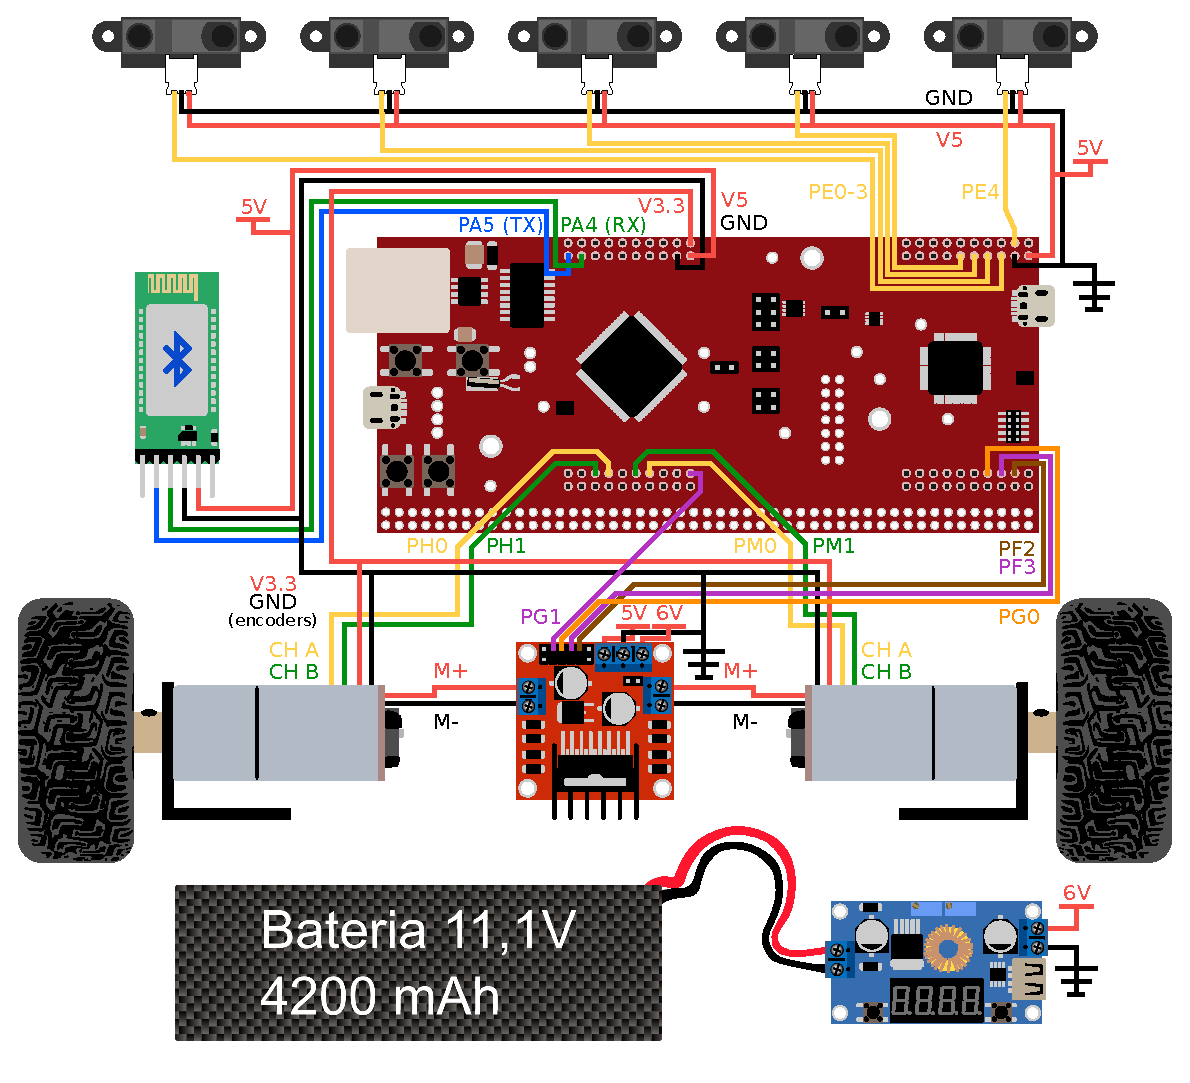
\includegraphics[trim =
		{0cm 0cm 0cm 0cm}, clip, scale=0.8]{Figuras/EsquemaCircuito.eps}};
	\end{tikzpicture}
}
\end{figure}
\end{frame}

\begin{frame}
	\begin{figure}[ht]
	\centering
\resizebox{0.35\linewidth}{!}{
	\begin{tikzpicture}
		\node[anchor=south west,inner sep=0] (image) at (0,0) {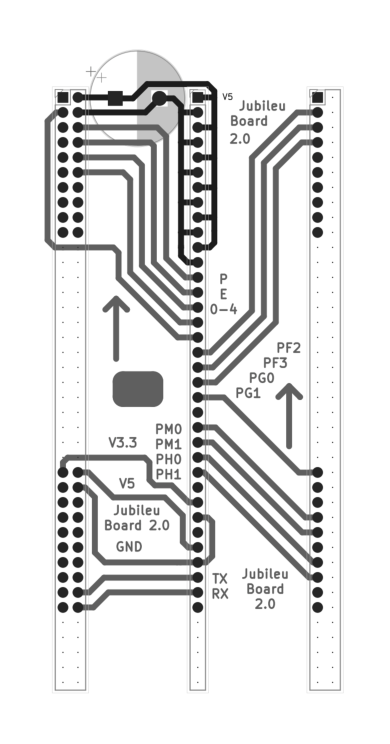
\includegraphics[trim =
		{0cm 0cm 0cm 0cm}, clip,scale=1]{Figuras/JubileuBoard.eps}};
	\end{tikzpicture}	
}
\end{figure}
\end{frame}
	
\begin{frame}
	\frametitle{Comunicação}
	\begin{block}{Interface por Linha de Comando}
		\begin{table}[ht]
\centering
\vspace{0.2 cm}
\resizebox{0.9\linewidth}{!}{
\begin{tabular}{|l|l|}
\hline
\textbf{Comando}       & \textbf{Descrição}                                                                                                                     \\ \hline
SUPERVISOR\_HIBRIDO    & \begin{tabular}[c]{@{}l@{}}Adota o controlador híbrido como a estratégia de \\ navegação utilizada\end{tabular}                        \\ \hline
SUPERVISOR\_FUZZY      & \begin{tabular}[c]{@{}l@{}}Adota o controlador \textit{fuzzy} como a estratégia de\\ navegação utilizada\end{tabular}                  \\ \hline
SETCOORDOBJ(X.XX,Y.YY) & Redefine a coordenada objetivo                                                                                                         \\ \hline
GETSTATE               & \begin{tabular}[c]{@{}l@{}}Utilizado para obter a resposta do estado do robô\\ ($x$, $y$ e $\theta$) a cada iteração, bem como o valor de seus\\ sensores \end{tabular}      \\ \hline
EXIT                   & \begin{tabular}[c]{@{}l@{}}Necessário para solicitar ao robô para que deixe \\ de informar seu estado a cada iteração\end{tabular}     \\ \hline
\end{tabular}
}
\end{table}	
	\end{block}
\end{frame}

%%%%%%%%%%%%%%%%%%%%%%% RESULTADO - SIMULACAO
\begin{frame}
	\frametitle{Resultado para Simulação - Controlador Híbrido}
	\begin{figure}[ht]
		\centering
		% fbox{}
		%\includegraphics[clip, 
%scale=0.058]{Figuras/simulacao_hibrido}
\resizebox{\columnwidth}{!}{
		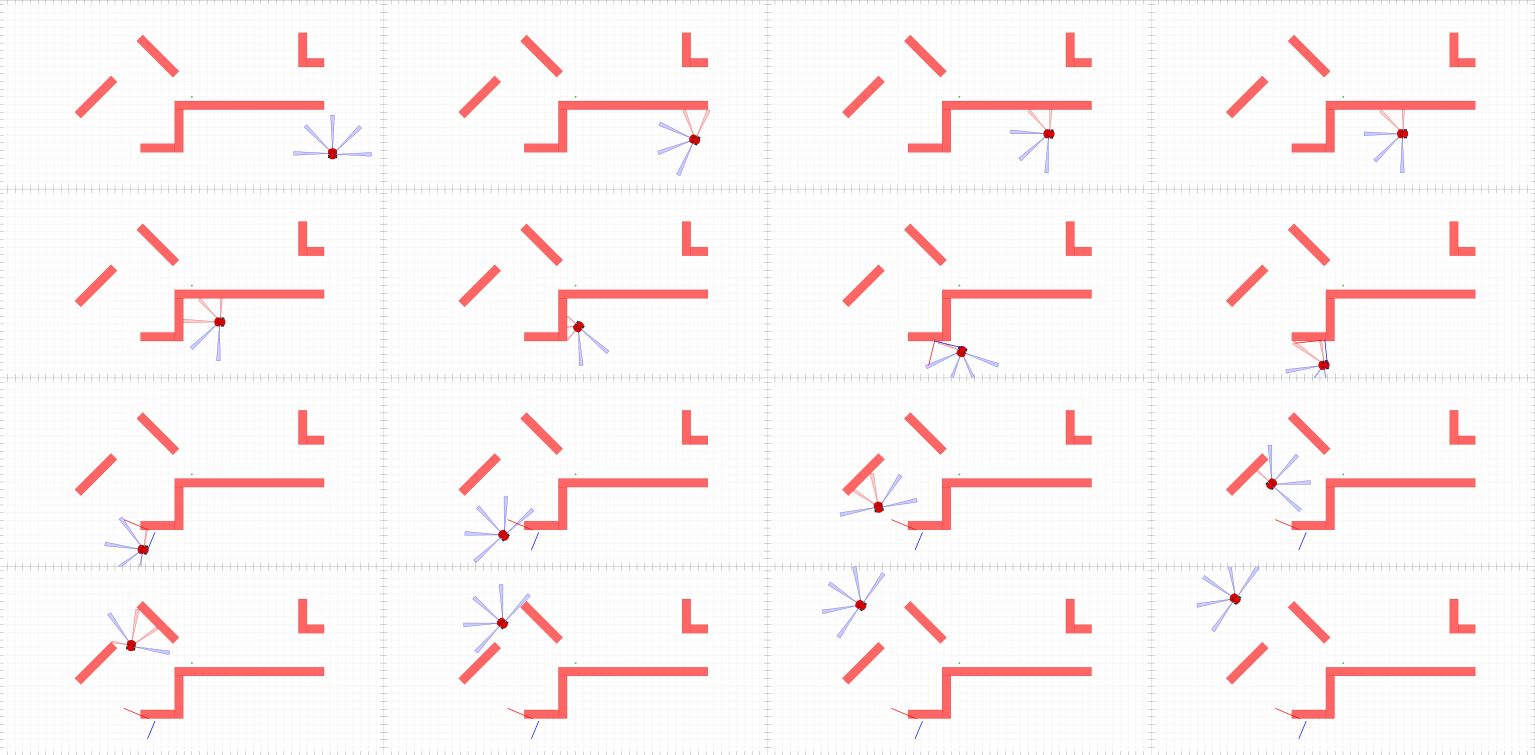
\includegraphics[clip, 
scale=0.29]{Figuras/simulacao_hibridoCompactado}
}
\end{figure}
\end{frame}

\begin{frame}
	\frametitle{Resultado para Simulação - Controlador Fuzzy}
	\begin{figure}[ht]
		\centering
		% fbox{}
		%\includegraphics[clip, 
%scale=0.058]{Figuras/simulacao_fuzzy}
\resizebox{\columnwidth}{!}{
		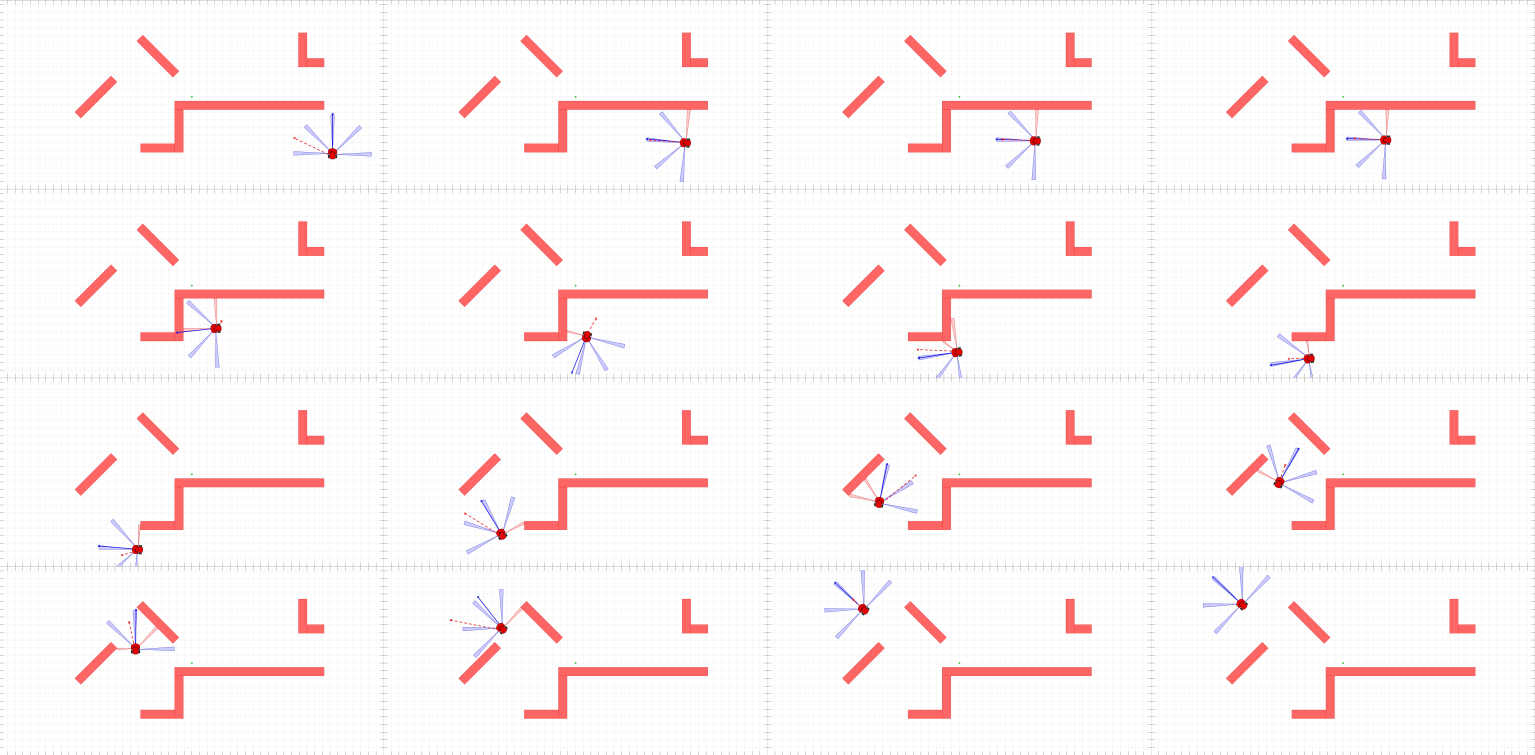
\includegraphics[clip, 
scale=0.29]{Figuras/simulacao_fuzzyCompactado}
}
\end{figure}
\end{frame}

%%%%%%%%%%%%%%%%%%%%%%% RESULTADO - ROBO
\begin{frame}
	\frametitle{Resultado Para o Robô - Controlador Híbrido}
	\begin{figure}[!ht]
\centering
\caption{Resultado do comportamento ``Ir Para Objetivo''}
\label{fig:resultadoImplementadoIPO}
		\centering
		% fbox{}
		%\includegraphics[clip, 
%scale=0.058]{Figuras/ComportamentoIPO}%
		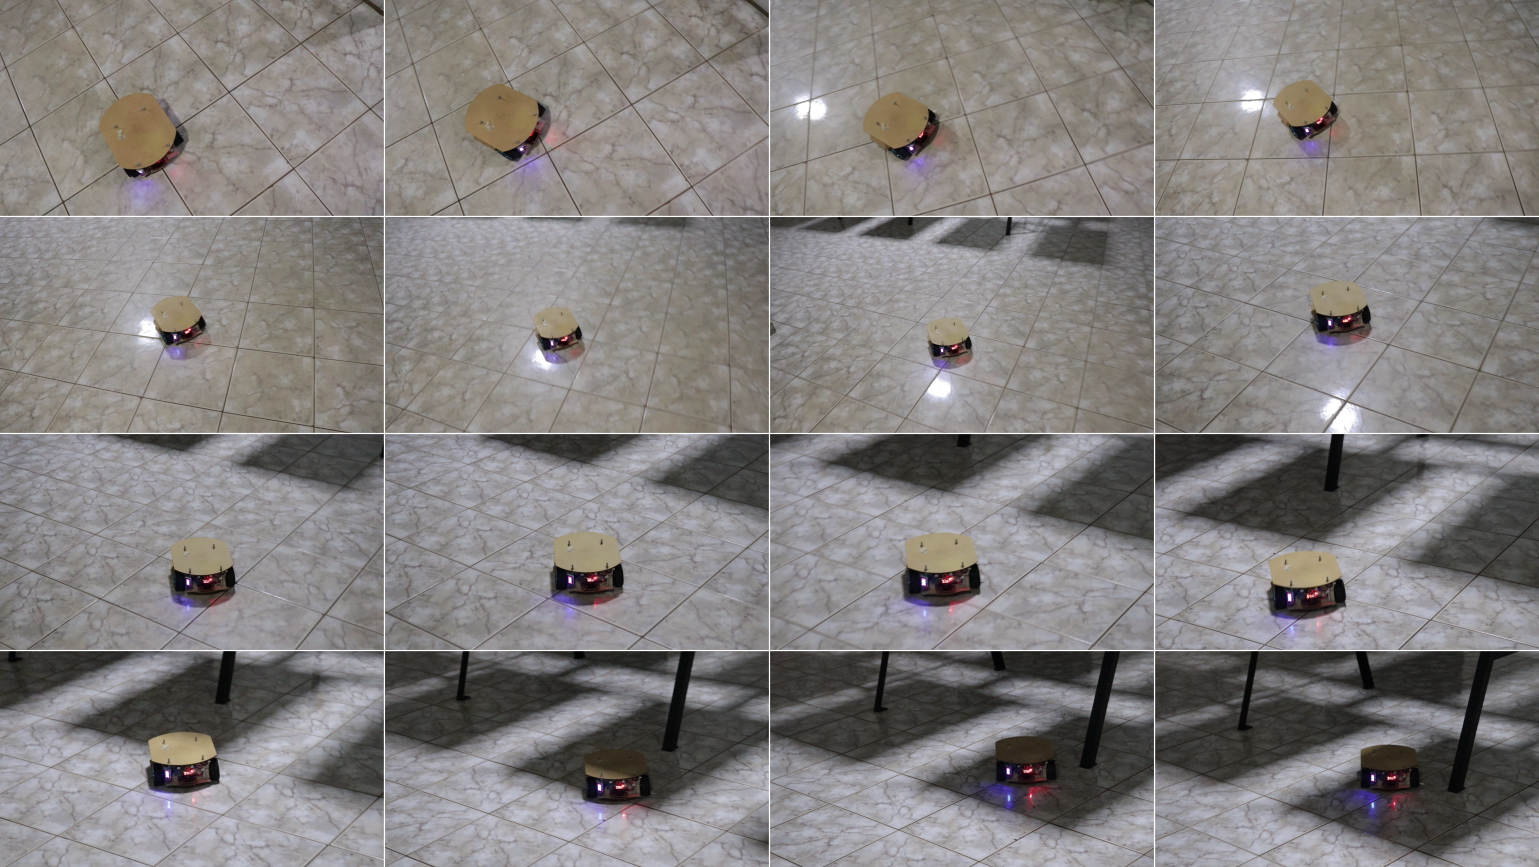
\includegraphics[clip, 
scale=0.29]{Figuras/ComportamentoIPOCompactado}%

	\textbf{Fonte: autoria própria}
\end{figure}
\end{frame}

\begin{frame}
	\frametitle{Resultado Para o Robô - Controlador Híbrido}
	\begin{figure}[!ht]
\centering
\caption{Resultado do comportamento ``Evitar Obstáculo''}
\label{fig:resultadoImplementadoEO}
		\centering
		% fbox{}
		%\includegraphics[clip, 
%scale=0.058]{Figuras/ComportamentoEO}%
		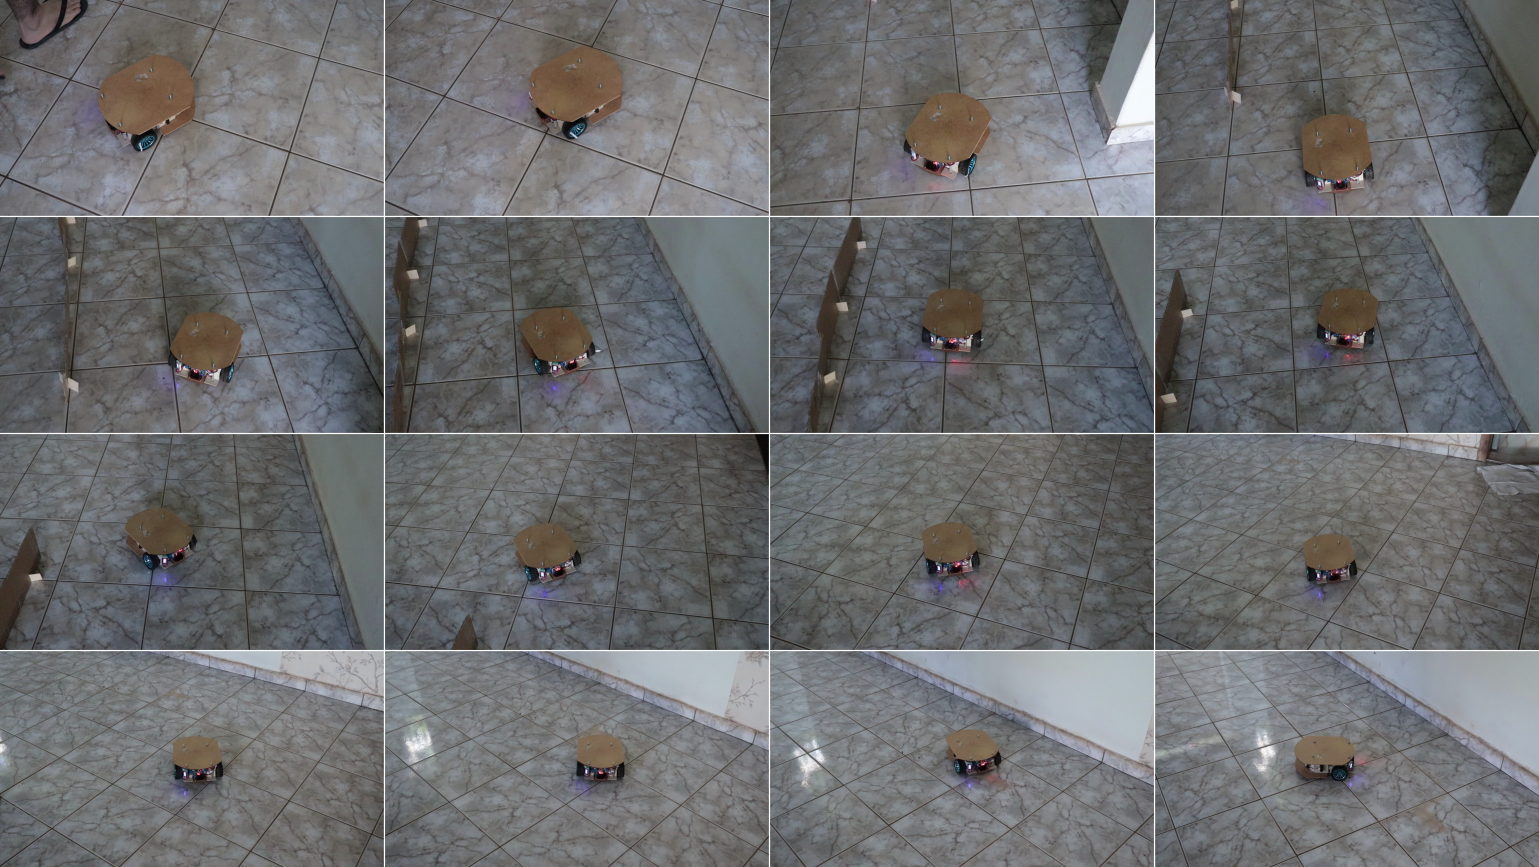
\includegraphics[clip, 
scale=0.29]{Figuras/ComportamentoEOCompactado}%

	\textbf{Fonte: autoria própria}
\end{figure}
\end{frame}

\begin{frame}
	\frametitle{Resultado Para o Robô - Controlador Híbrido}
	\begin{figure}[!ht]
		\centering
		% fbox{}
		%\includegraphics[clip, 
%scale=0.058]{Figuras/ComportamentoIPO_E_EO}%
\resizebox{\columnwidth}{!}{
		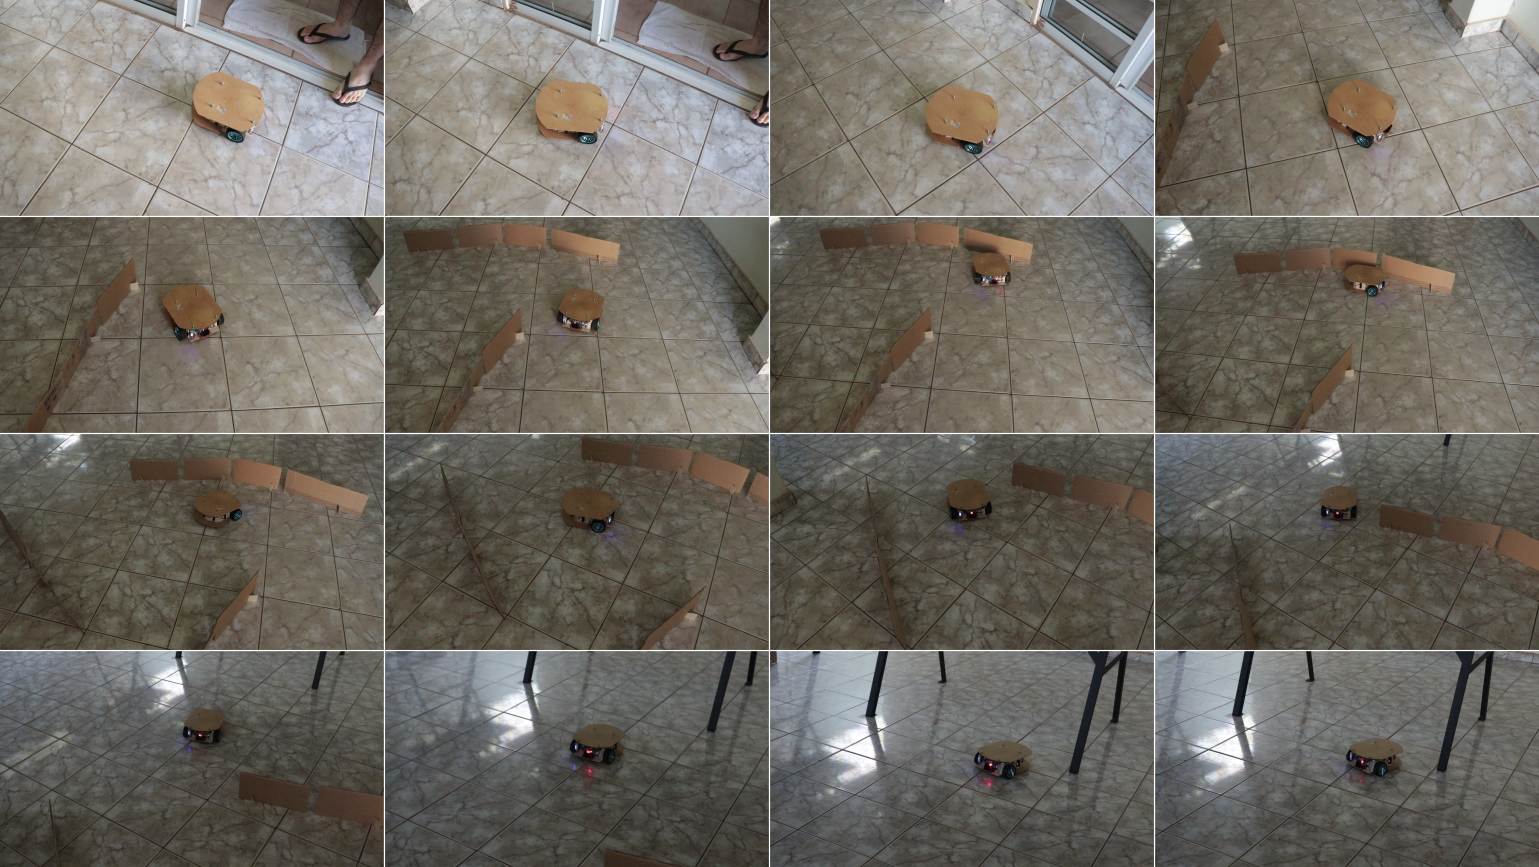
\includegraphics[clip, 
scale=0.29]{Figuras/ComportamentoIPO_E_EOCompactado}%
}
\end{figure}
\end{frame}

\begin{frame}
	\frametitle{Resultado Para o Robô - Controlador Híbrido}
	\begin{figure}[!ht]
\centering
\caption{Resultado do comportamento ``Seguir Parede''}
\label{fig:resultadoImplementadoSP}
		\centering
		% fbox{}
		%\includegraphics[clip, 
%scale=0.058]{Figuras/ComportamentoSP}%
		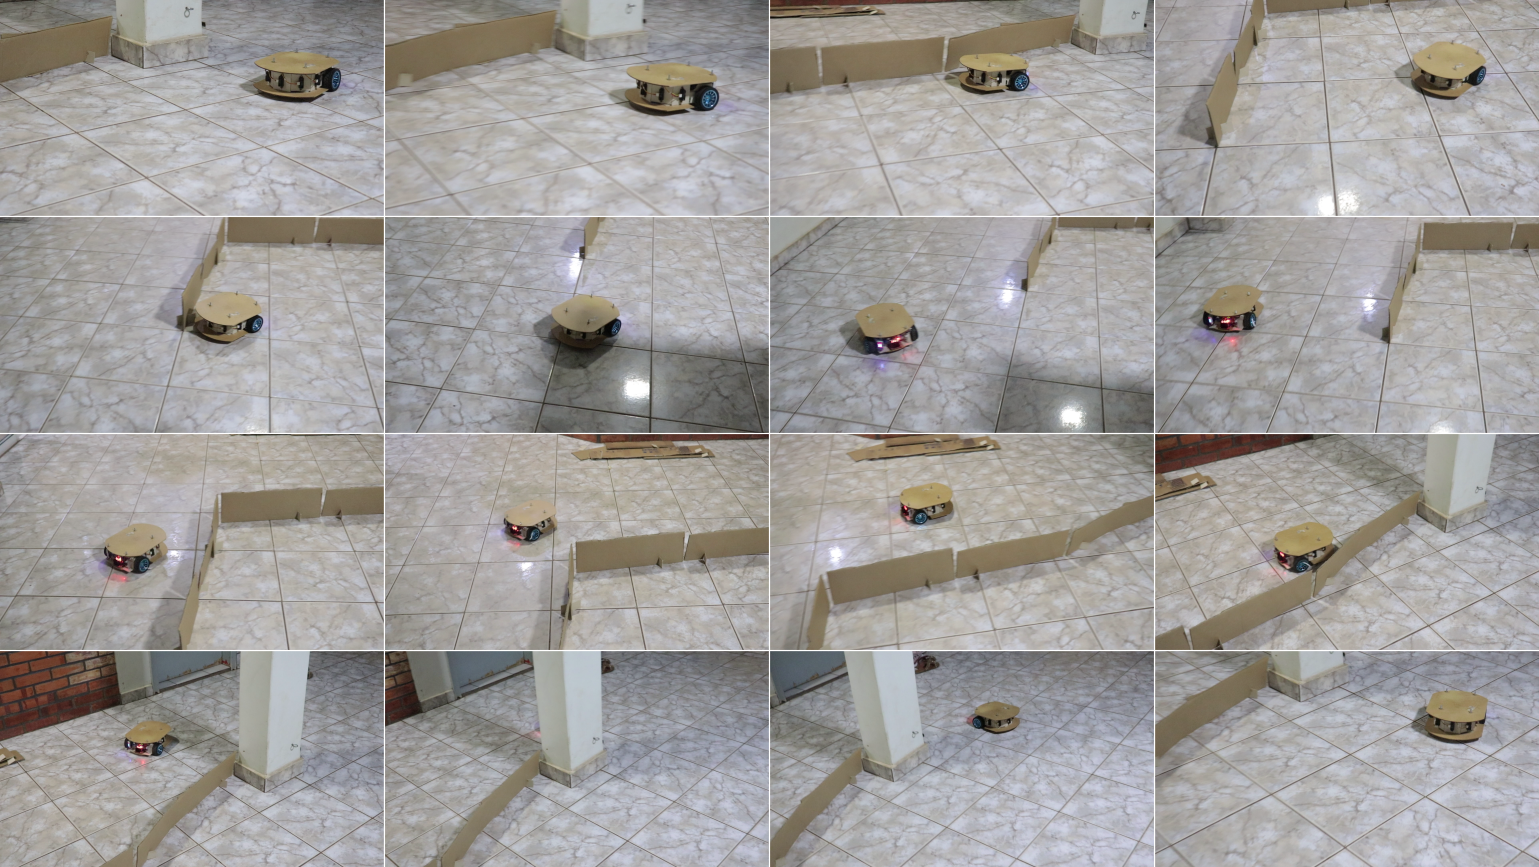
\includegraphics[clip, 
scale=0.29]{Figuras/ComportamentoSPCompactado}%

	\textbf{Fonte: autoria própria}
\end{figure}
\end{frame}

\begin{frame}
	\frametitle{Resultado Para o Robô - Controlador Híbrido}
	\begin{figure}[ht]
\centering
\caption{Resultado implementado para o controlador híbrido}
\label{fig:resultadoImplementadoHibrido}
		\centering
		% fbox{}
		%\includegraphics[clip, 
%scale=0.058]{Figuras/hibrido}%
		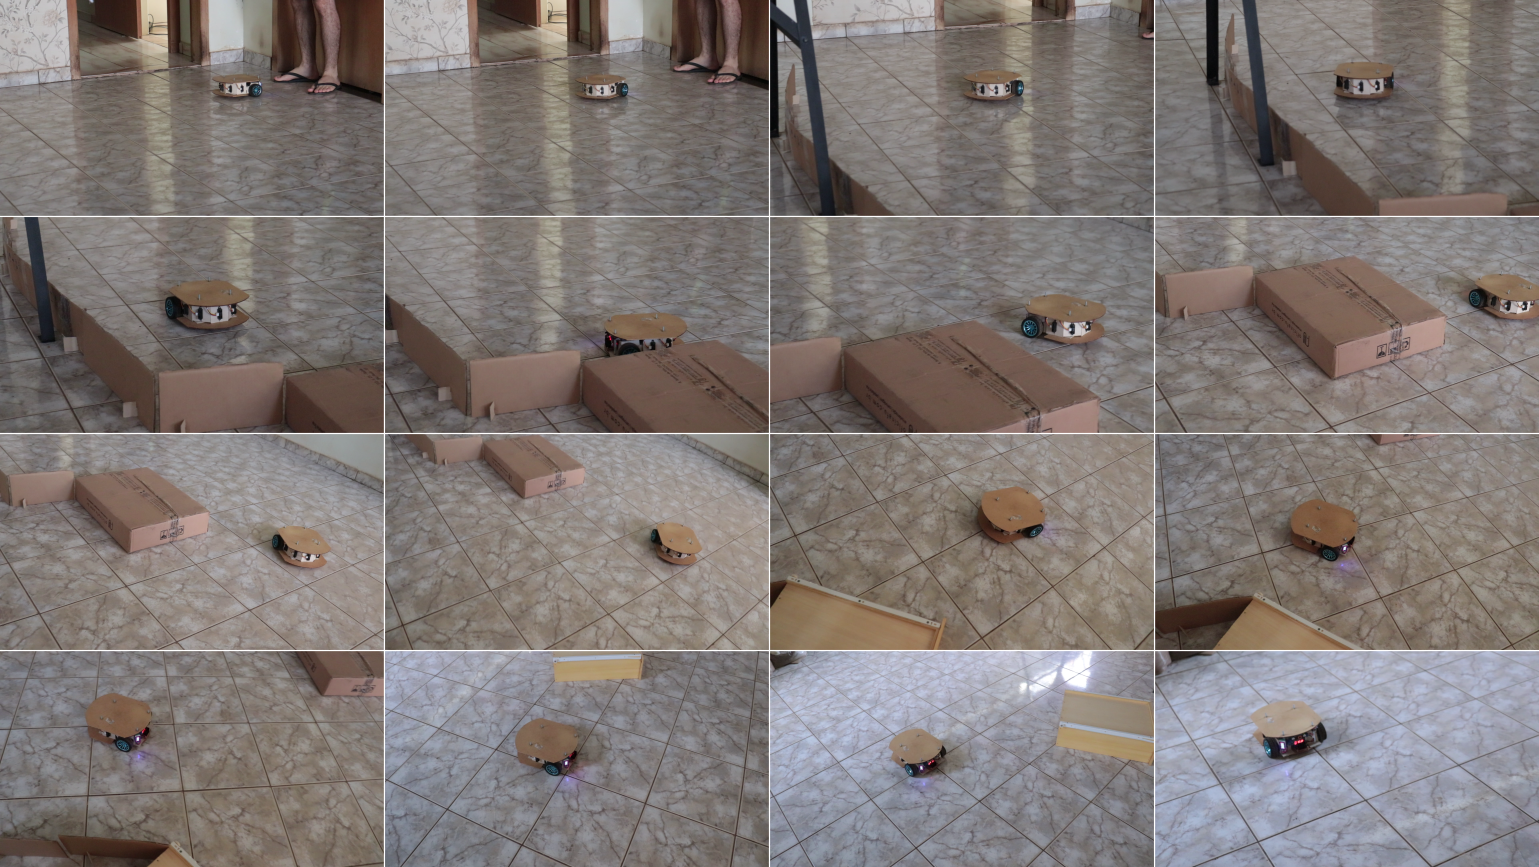
\includegraphics[clip, 
scale=0.29]{Figuras/hibridoCompactado}%

	\textbf{Fonte: autoria própria}
\end{figure}
\end{frame}

\begin{frame}
	\frametitle{Resultado Para o Robô - Controlador Fuzzy}
	\begin{figure}[ht]
\centering
\caption{Resultado implementado para o controlador \textit{fuzzy}}
\label{fig:resultadoImplementadoFuzzy}
		\centering
		% fbox{}
		%\includegraphics[clip, 
%scale=0.058]{Figuras/fuzzy}
		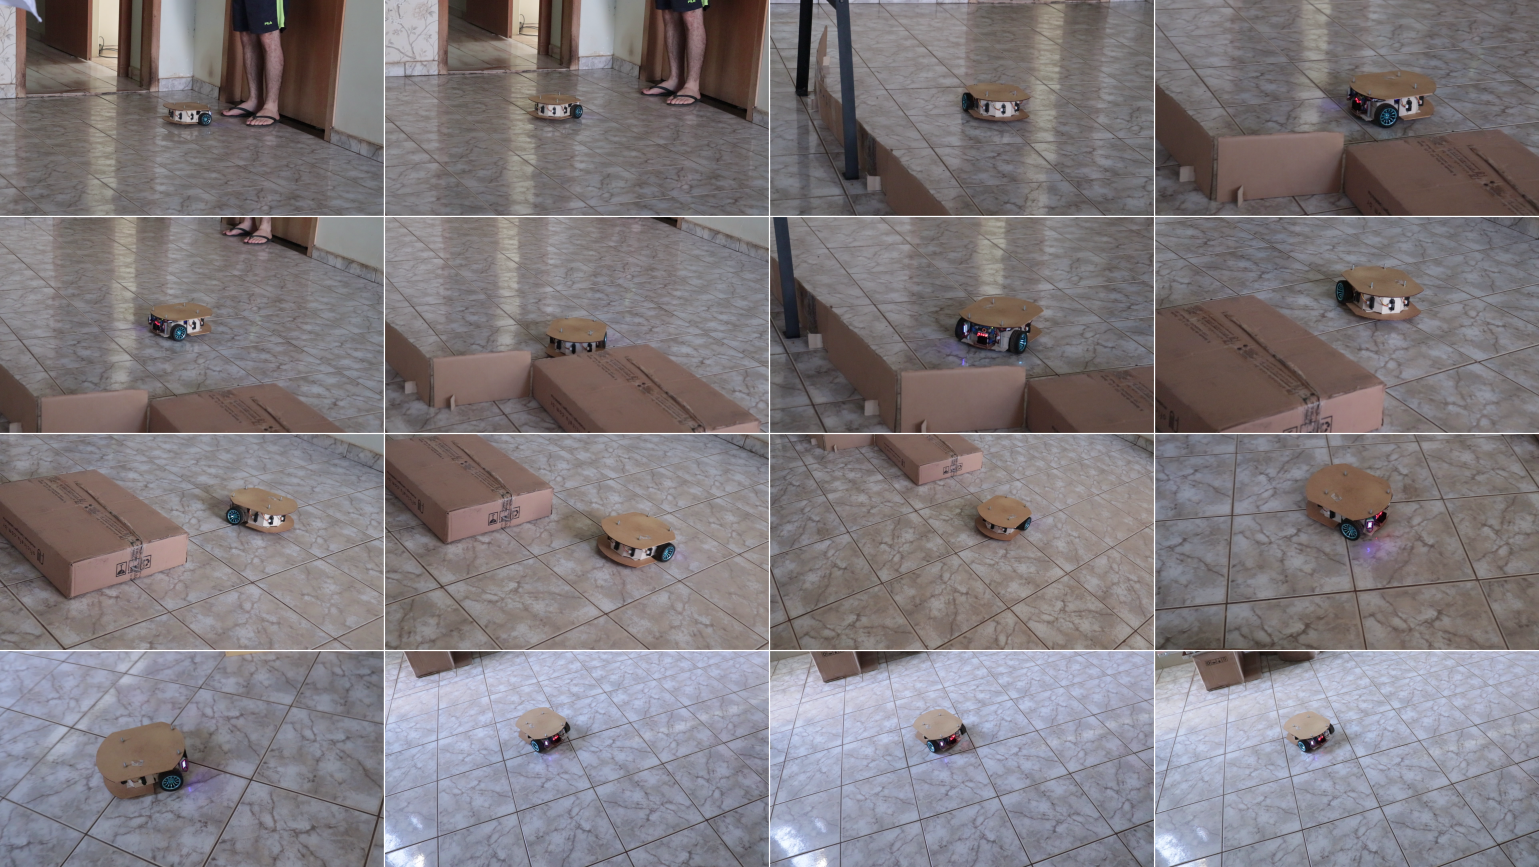
\includegraphics[clip, 
scale=0.29]{Figuras/fuzzyCompactado}

	\textbf{Fonte: autoria própria}
\end{figure}
\end{frame}
